\documentclass{article}
\usepackage[fleqn]{amsmath}
\usepackage{amssymb,graphicx,color,graphicx,slashed, microtype, parskip, enumitem, extarrows, needspace}
%\usepackage[utf8x]{inputenc}
\usepackage[top=1.5cm, bottom=1.5cm, right=6cm, left=1.5cm, heightrounded, marginparwidth=5cm, marginparsep=0.5cm]{geometry}

\hbadness = 10000
\hfuzz=100pt 
    
\usepackage{marginnote}
\renewcommand*{\marginfont}{\footnotesize}

\usepackage{hyperref}
\hypersetup{colorlinks=true, urlcolor=NavyBlue, bookmarksdepth=3}

\makeatletter\newcommand{\@minipagerestore}{\setlength{\parskip}{\medskipamount}}\makeatother

% =============== Index ===========================

\usepackage[nonewpage]{imakeidx}
\makeindex

% =============== Color Definitions ===============
    
\usepackage[svgnames]{xcolor}
\colorlet{ColorTitle}{Black}
\colorlet{ColorSectionName}{Black}
\colorlet{ColorBoxFG}{Gray}
\colorlet{ColorBoxText}{Black}
\colorlet{ColorBoxBG}{White}


% =============== Title Style ===============
    
\usepackage{titling} % Allows custom title configuration
    
\newcommand{\HorRule}{\color{ColorTitle}\rule{\linewidth}{1pt}} % Defines the gold horizontal rule around the title
    
\pretitle{
    \vspace{-50pt} % Move the entire title section up
    \HorRule\vspace{9pt} % Horizontal rule before the title
    \fontsize{27}{36}\usefont{OT1}{phv}{b}{n}\selectfont
    \color{ColorTitle} % Text colour for the title and author(s)
}
    
\posttitle{\par\vskip 15pt} % Whitespace under the title
    
\preauthor{\fontsize{17}{0}\usefont{OT1}{phv}{m}{n}\selectfont\color{ColorTitle}} % Anything that will appear before \author is printed
    
\postauthor{\par\HorRule}

\newcommand{\COURSENAME}{\href{http://phyw.people.ust.hk/teaching/PHYS2022-2015/}{\textcolor{black}{PHYS 2022}}}
\newcommand{\YW}{\href{http://phyw.people.ust.hk/}{\textcolor{black}{Yi Wang}}}
\newcommand{\PHYS}{\href{http://physics.ust.hk}{\textcolor{black}{Department of Physics}}}
\newcommand{\HKUST}{\href{http://www.ust.hk/}{\textcolor{black}{HKUST}}}
\author{\COURSENAME, \YW, \PHYS, \HKUST}

\date{}

% =============== Section Name Style ===============
    
\usepackage{titlesec}
    
\titleformat{\section}
    {\fontsize{15}{20}\usefont{OT1}{phv}{b}{n}\color{ColorSectionName}}
    {\thesection}{1em}{}
    %[{\vspace{0.2cm}\titlerule[0.8pt]}]
    
\titleformat{\subsection}
    {\fontsize{14}{20}\usefont{OT1}{phv}{m}{n}\color{ColorSectionName}}
    {\thesubsection}{1em}{}
    
\titleformat{\subsubsection}
    {\fontsize{12}{20}\usefont{OT1}{phv}{m}{n}\color{ColorSectionName}}
    {}{0em}{}
      
\setcounter{secnumdepth}{4}
        
% =============== Box Style ===============
    
\usepackage[most]{tcolorbox}
    
\newtcolorbox{tbox}[1]{
    colback=ColorBoxBG, colframe=ColorBoxFG, coltext=ColorBoxText,
    sharp corners, enhanced, breakable, parbox=false,
    before skip=1em, after skip=1em,
    title={#1}, fonttitle=\usefont{OT1}{phv}{b}{n}, 
    attach boxed title to top left={yshift=-0.1mm}, boxed title style={sharp corners, colback=ColorBoxFG, left=0.405cm},
    rightrule=-1pt,toprule=-1pt, bottomrule=-1pt
}

\newtcolorbox{mtbox}[1]{
    colback=ColorBoxBG, colframe=ColorBoxFG, coltext=ColorBoxText,
    sharp corners, enhanced, breakable, parbox=false,
    before skip=1em, after skip=1em,
    title={#1}, fonttitle=\usefont{OT1}{phv}{b}{n},
    attach boxed title to top left={yshift=-0.1mm}, boxed title style={sharp corners, colback=ColorBoxFG, left=0.15cm},
    rightrule=-1pt,toprule=-1pt, bottomrule=-1pt, 
    left=0.5em
}

% =============== tikz has to be loaded after xcolor
\usepackage{tikz}

\newcommand*\enumlabel[1]{\tikz[baseline=(char.base)]{
			\node[shape=rectangle,inner sep=2pt,fill=ColorBoxFG] (char) 
			{\fontsize{7}{20}\usefont{OT1}{phv}{b}{n}{\textcolor{ColorBoxBG}{#1}}};}}

% =============== Useful shortcuts ===============

\newcommand\wref[1]{{\hypersetup{linkcolor=white}\ref{#1}}}  

\newcommand{\textbox}[2]{
    \begin{tbox}{#1}
        #2
    \end{tbox}
}

\newcommand{\mtextbox}[2]{\marginnote{
    \begin{mtbox}{#1}
        #2
    \end{mtbox}}
}

\newcommand{\mnewline}{\vspace{0.5em}\newline}

\newcommand{\titem}[1]{
    \begin{itemize}[label=\color{ColorBoxFG}$\blacktriangleright$, leftmargin=0mm, labelsep=0.27cm, topsep=0.5em
        %, itemsep=1ex
        ]
        #1
    \end{itemize}
}

\newcommand{\mtitem}[1]{
    \begin{itemize}[label={\color{ColorBoxFG}$\blacktriangleright$}, leftmargin=0mm, labelsep=1mm, topsep=0.5em
        %, itemsep=1ex
        ]
        #1
    \end{itemize}
}

\newcommand{\itembox}[3]{
    \begin{tbox}{#1}
        #2
        \titem{#3}
    \end{tbox}
}

\newcommand{\mitembox}[3]{
    \marginnote{
    \begin{mtbox}{#1}
        #2
        \mtitem{#3}
	\end{mtbox}
    }
}

\newcommand{\tenum}[1]{
    \begin{enumerate}[label=\protect\enumlabel{\arabic*}, leftmargin=0mm, labelsep=0.265cm, topsep=0.5em
        %, itemsep=1ex
        ]
        #1
    \end{enumerate}
}

\newcommand{\enumbox}[3]{
    \begin{tbox}{#1}
        #2
        \tenum{#3}
    \end{tbox}
}

\newcommand{\twocol}[5]{
    \begin{minipage}[t][][b]
        {#1\textwidth}
        #4        
    \end{minipage}
    \hspace{#2\textwidth}
    \begin{minipage}[t][][b]
        {#3\textwidth}
        #5
    \end{minipage}
}

\newcommand{\cg}[2]{
    \begin{center}
        \includegraphics[width=#1\textwidth]{#2}
    \end{center}
}

\newcommand{\tbar}{
    ~\newline
    {\color{ColorBoxFG}
    \hbox to 0.15\textwidth{\leaders\hbox to 5pt{\hss  \hss}\hfil} 
    \hbox to 0.7\textwidth{\leaders\hbox to 5pt{\hss . \hss}\hfil}}
    \mnewline
}

% =============== Filter unwanted warnings
\usepackage{silence}
\WarningsOff[tcolorbox]
\hbadness=1000000


\usepackage{wasysym}
\graphicspath{{1_fig/}}
\title{第一章\ 狭义相对论}

\usepackage{ctex}


\begin{document}

\maketitle

让我们从一个思想实验开始我们探索物理的奇妙旅程——王二乘坐宇宙飞船前往距离我们5光年远的一颗恒星,他到达后将立即返回地球。王三送他走并等他回来。假设宇宙飞船的运行速度几乎与光速 $c$ 一样快,例如 $v=0.995c$
\cg{0.7}{spaceship5}

令人惊讶的是,在 $v\sim c$ 处,事物的行为与我们的日常经验(也就是牛顿力学)截然不同。让我们看看他们发现的一些神奇的事实:

\mitembox{对于时空的理解}{
	随着我们对自然更好的了解,我们对时空也有了更深入的理解。到目前为止,科学家们依然在努力的探索。
	}{
	\item 牛顿力学: 空间和时间对于物质来说是绝对独立的。
	\item 狭义相对论:空间和时间是统一的,并且取决于观察者的运动(就像物体的相对方向会随着观察者的转动而改变)。
	\item 广义相对论: 空间和时间可以被物体弯曲。
	\item 量子引力(推测):空间和时间可能是从全息和量子纠缠中演生出来的。我们还没有完全理解它,但是我们从中得到的这些线索是深刻的。

}

\itembox{王三对王二旅行的观察}{}{
	\item 王三给王二写了一封信,王二大约在同一时间也给王三写了一封信。王三认为他的信写的更早,同时王二也坚持认为他自己的信写得更早。他们考虑到了光需要时间才能传播,但即使如此,他们也无法解决这个纷争。

	\item 王三发现当 $v\sim c$ 时,飞船变得更重了,王二需要越来越多的能量来使飞船加速。
	\item 当王二回来时,王三已经过去了 10 年。但对于王二来说,他的时钟,他的感觉,关于他的一切都表明,仅仅过去了一年。
} 

这里发生了什么?学完这部分内容,你就会发现,还有更多神奇的事情。事实上,我们必须以一种与我们天真的想法截然不同的方式来思考空间和时间。

\section{相对性原理}\label{sec:principles-relativity}

\subsection{伽利略变换}

想象一下:
\marginnote{“向外看”指的是通过任何方式与汽车外部的连接,比如使用光、声、引力波等。我们忽略地球的自转,从而我们可以认为王二和王三处于惯性坐标系(也就是他们的运动是匀速的)。
}
在图~\ref{fig:grel}中,王二在一辆封闭的汽车中以恒定速度 $\mathbf{v}$ 相对于地面移动。如果王二不看车外,他怎么会发现他在地面上移动呢?


答案是如果王二不看车外,无论他尝试什么活动/实验,他都发现与汽车没有移动时没有区别。用物理学的语言来说,他这时探索到的自然界的定律与他不动时探索到的定律是完全相同的。

在1632年,伽利略说这对所有物理定律和所有惯性系都是正确的。这被称为伽利略相对性原理。令人惊叹的是,据我们所知,这一拥有近 400 年历史的原理在现在仍然适用。
 
\begin{figure}[htbp] 
	\centering
	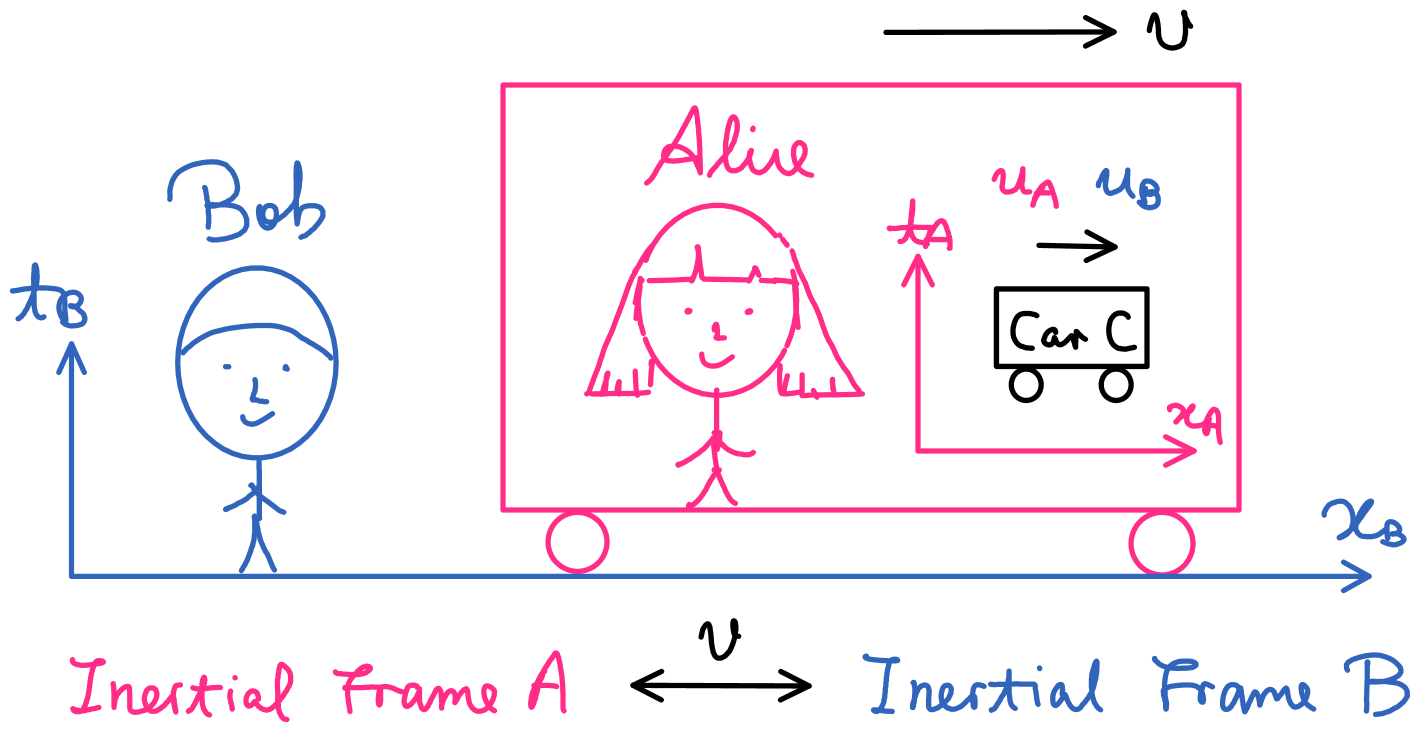
\includegraphics[width=0.7\textwidth]{galileo_relativity}
	\caption{\label{fig:grel} 王二有他的时间 $t_A$ 和空间 $x_A$;王三也有他的时间 $t_B$ 和空间坐标$x_B$。 王三和王二的相对速度为 $v$(因为王二站在一辆移动的大车上)。一辆小型汽车 C 的速度相对于王二为 $u_A$ ,相比于王三为 $u_B$。为简单起见,我们只展示$x$方向上的运动,而不考虑其他空间维度 $y$ 和 $z$ 的运动。}
\end{figure} 

\mtextbox{伽利略的理论是简单而微不足道的吗?}{
		现在$(\mathbb{R})$看起来很简单。 这是因为我们已经学习了牛顿力学。 
		\mnewline
	但在伽利略(1564-1642)时代,人们还没有加速度的概念,他靠肉眼来进行天文学的探索。当时的人们更相信地心模型而不是日心说(地球围绕太阳运动)。 地心模型的一个论点是,如果地球移动得很快,我们就会从地球上掉下来,而 $(\mathbb{R})$ 表明它不会发生。
		\mnewline
此外,现在我们还知道 $(\mathbb{R})$在牛顿力学不成立的情况下仍然成立,包括在狭义相对论成立的时候以及其他的一些情况。}
\textbox{伽利略的相对性原理}{
	物理定律在所有惯性系中都是相同的 \index{伽利略的相对性原理}
	\tcblower
因为会多次提到伽利略的相对性原理,所以在此让我们把伽利略的相对性原理简写为 $(\mathbb{R})$ 。这里有一些和$(\mathbb{R})$等效的语句:
	\titem{
		\item 运动是相对的。
		\item 没有绝对意义上的“运动”。
	}
我们把从一个惯性系到另一个惯性系通过相对运动的变化,称为“推动”变换。因此我们也可以说
\titem{
		\item 定律不会因“推动”变换,即惯性系的不同而改变。
	}
}

\textbox{牛顿力学和伽利略相对论的一致性}{
在 图~\ref{fig:grel} 中,牛顿第二定律(物理定律)对于王三和王二是否是相同的? 要证明这一点,请注意参考系之间的关系是	\begin{align}\label{eq:newtontx}
		t_B = t_A~, \qquad
		x_B = x_A + v t_A~.
	\end{align}
	王二参考系中的牛二定律是 $F = m a_A$。 那么在王三的参考系中呢?王三选取王二 的方程并将其转换为用王三参考系中的物理量表示:\marginnote{符号表示: $\dot x \equiv dx/dt$, $\ddot x \equiv d^2x/dt^2$. 
	\mnewline
你能尝试验证牛顿第一定律和第三定律吗?}
	\begin{align}
		F = m a_A = m \ddot{x}_A = m \ddot{x}_B = m a_B~.
	\end{align}
因此,王二在他的坐标系中确实具有相同的牛二定律。

以便以后的使用,我们总结出牛顿力学中的速度相加规则可以从同一个坐标系变换 \eqref{eq:newtontx} 导出:	\begin{align}
		\label{eq:vel_add_newton} 
		u_A = \dot x_A~,
		\qquad
		u_B = \dot x_B = u_A + v~. 	  
	\end{align}
}

从上文中,我们发现: $(\mathbb{R})$ 和牛顿力学可以得出相同的结果。 然而,牛顿力学并不是唯一满足 $(\mathbb{R})$ 的体系。 为了更好的说明这一点,并引出爱因斯坦的相对论,让我们先来介绍另一个基本的物理现象。

\subsection{光的速度}

\mtextbox{(拓展内容) 对于光速有限的观测}{
	早在 1676 年,R{\o}mer 就注意到实际观测到的木星卫星 Io 的日食在发生在地球L、K、G 和 F 位置时与计算的时间存在差异。这被解释为 : 光需要时间穿过 LK 和 GF 区间。
	\newline
	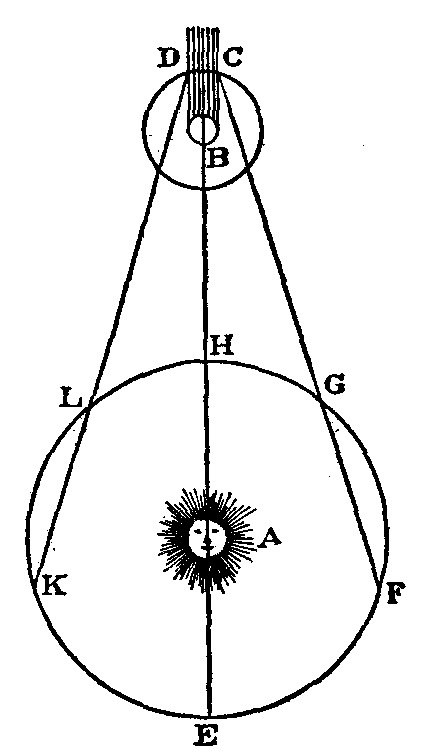
\includegraphics[width=\textwidth]{Romer_light}
} 

当我们打开灯时,光线“立即”充满了整个房间。在我们的日常生活中,光速是如此之快,以至于我们通常会忽略光所需的传播时间。 然而,光速是究竟是无限的,还是有限的呢?

科学家们设计了很多精细的实验来证明光速实际上是有限的,光的速度大约是 $c\simeq 3\times 10^8 $m/s。 右侧方框概述了天文学的第一个观察结果。 如今,光速的有限性不仅成为了现代物理的事实,而且在未来的应用中也有着巨大的前景。

\textbox{光速的精确值}{ \index{光速}
	光速 $c$ 有一个精确的值: $c = 299,792,458\mbox{m/s}$. 
	
这个事实是不是让你感到了惊讶? 通常,物理常数是通过测量确定的。 测量总是有误差的。 那么,$c$ 怎么会有一个准确的值呢?	
	\tcblower
	
米的现代定义(自 1983 年以来)是光在 1 秒内传播的距离(也就是$c$ 的值)。 事实上,在历史上(1889-1960)米是由一个被称为“国际原型米”的真实物体定义的。 但是使用真实物体定义仪表有很多缺点,包括	\titem{
		\item 人们必须与原型(或它的副本)进行比较以确定长度。
		\item 副本的准确性受到当时技术的限制。
		\item 原型的长度随时间略有变化。 甚至它可能会损坏。
	}
通过使用自然常数 $c$ 来定义米的概念,所有人都可以得到一米的长度。 误差仅受他/她实验精度的限制。 此外,时间和质量的现代定义也使用了量子力学的基本性质,它们是通过原子频率和普朗克常数定义的。}

现在,让我们来到这一节的重点,也就是爱因斯坦狭义相对论的基石。

\marginnote{我们已经说过光速是在现代定义长度的一种方式。 但是现在,让我们先回到 1900 年代初期,人们仍然考虑以单位时间内移动的距离来衡量的光速,以及距离和时间符合常识的定义。}
\textbox{来自移动光源的光的速度是多少?}{
	王三拿着蜡烛。 王三的蜡烛发出的光相对于王三的速度是 $c_3 = c$ 。 
	王二在一辆车里以相对于王三 $v$ 的速度运动。 王二也拿着一个蜡烛,我们来思考:
	\titem{
		\item 王二的蜡烛发出的光相对于王二的速度$c_2$ 是多少?
		\item 王二的蜡烛发出的光相对于王三的速度$c_3$ 是多少?(注:此处 $c_3$ 与上文 $c_3$ 代表的是不同光源相对于王三的速度)
	}

	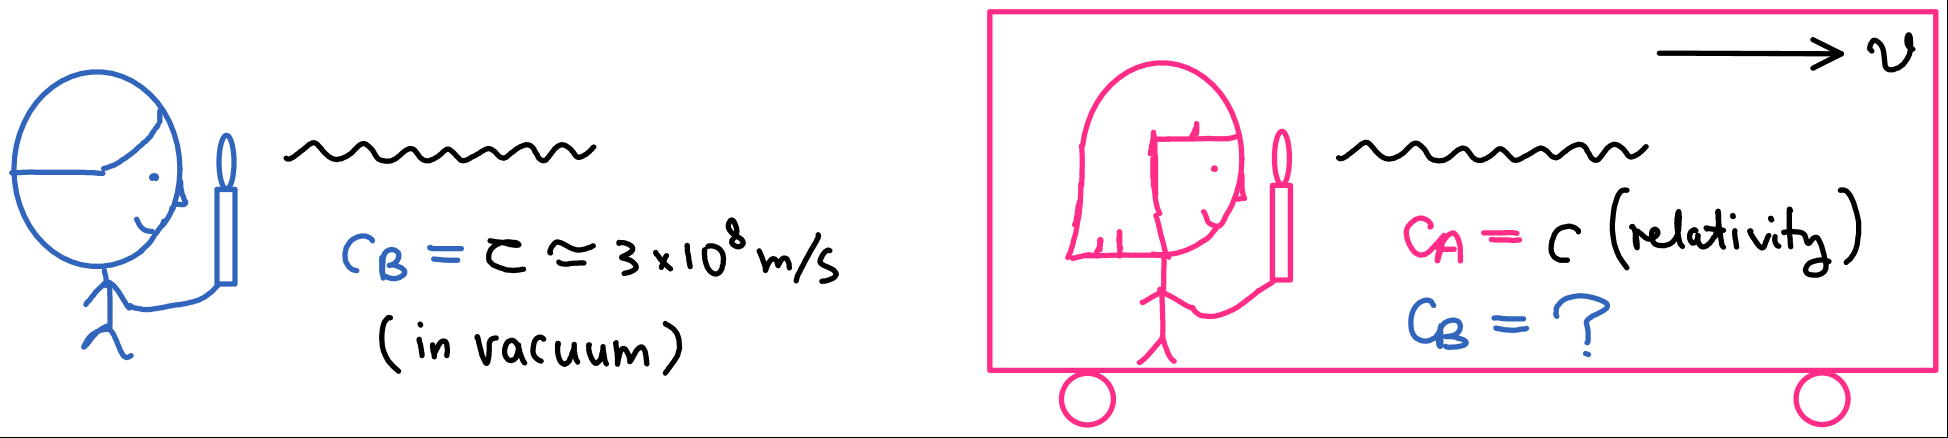
\includegraphics[width=0.6\textwidth, trim={0 3pt 3pt 0}, clip]{light}

	\tcblower

我们可以立即从 $(\mathbb{R})$ 得到 $c_A=c$。 否则王二就会通过测量到不同的光速值且不与汽车外部互动来知道他正在移动。 那么 $c_B$ 相对于王二的速度又是多少呢?}

我们可能会天真地得到 $c_B = c_A + v = c + v$ 通过牛顿力学中计算相对速度的原理。 \eqref{eq:vel_add_newton}. 而且这些看起来非常的正常 -- 在我们的日常生活中 (速度远小于光速): 如果王二在一辆相对于王三以速度 $v\ll c$ 运动的车里, 并相对王二自己以速度 $u_A$ 扔了一个球, 那么球相对于王三的速度就是 $u_B = v+u_A$.

然而,光传播的速度是由麦克斯韦方程推导出来的。 经过计算得到$c_B = c$! 下面的方框为您推导出了这个令人惊讶的事实。 推导需要使用多变量微积分,需要一些数学基础,因此,如果读者看不懂这些推导,您完全可以选择跳过它。

\mtextbox{麦克斯韦和相对论}{
事实上,隐藏在麦克斯韦方程组中的对称性已经暗示了爱因斯坦的狭义相对论。 光速不变只是其结果。 这种对称性被称为洛伦兹变换,是在爱因斯坦建立狭义相对论之前的 1887-1905 年间由 Voigt、Lorentz、Larmor 和 Poincare 提出的。 我们将在 \ref{sec:lorentz} 部分从机械的角度来讨论洛伦兹变换。}

\textbox{(拓展内容)由麦克斯韦方程组得出光速}{\index{speed of light from Maxwell equations}

	让我们来看王三的参考系。具有真空磁导率 $\mu_0$ 和介电常数 $\epsilon_0$ 的麦克斯韦方程为:

	\begin{minipage}{0.4\textwidth}
		\begin{align}
			\label{eq:mnde} \nabla \cdot  \mathbf{E} & = \frac{\rho}{\epsilon_0} ~,
		\end{align}
	\end{minipage}\hspace{0.1\textwidth}
	\begin{minipage}{0.45\textwidth}
		\begin{align}
			\label{eq:mndb}  \nabla \cdot  \mathbf{B} & = 0 ~,
		\end{align}
	\end{minipage}
	
	\begin{minipage}
		{0.4\textwidth}
		\begin{align}
			\label{eq:mnte} \nabla \times \mathbf{E} &= -\frac{\partial \mathbf{B}}{\partial t} ~,
		\end{align}
	\end{minipage}\hspace{0.1\textwidth}
	\begin{minipage}
		{0.45\textwidth}
		\begin{align}
			\label{eq:mntb} \nabla \times \mathbf{B} &= \mu_0 \left [ \mathbf{J} + \epsilon_0 \frac{\partial \mathbf{E}}{\partial t} \right ]~.
		\end{align}
	\end{minipage}\medskip

当我们研究光的传播时,我们考虑真空环境下的麦克斯韦方程。 因此电荷密度$\rho=0$,电流$\mathbf{J}=0$。 为了消除 $\mathbf{E}$ 并仅获得 $\mathbf{B}$ 的方程,我们使用以下技巧:让我们将\eqref{eq:mntb}的左边和右边同时进行$\nabla\times (\cdots)$ 的运算 ,得到:

	\begin{align} \nonumber
		\nabla\times\mbox{LHS} = \nabla\times(\nabla\times \mathbf{B})
		\xlongequal{\mbox{math identity}} \nabla (\nabla\cdot \mathbf{B}) - \nabla^2 \mathbf{B} \xlongequal{\mbox{using Eq.~\eqref{eq:mndb}}}
		- \nabla^2 \mathbf{B} ~,
	\end{align} 
	\begin{align} \nonumber
		\nabla\times\mbox{RHS} =  \mu_0\epsilon_0 \frac{\partial}{\partial t} (\nabla \times \mathbf{E}) 
		\xlongequal{\mbox{using Eq.~\eqref{eq:mnte}}} -\mu_0\epsilon_0 \frac{\partial^2}{\partial t^2} \mathbf{B} ~.
	\end{align}
	\mtextbox{相速度}{相速度可以从 \eqref{eq:maxwell_wave} 中的相位因子 $\cos[k(x-ct)]$ 得到。 这可以通过分析下图中的一个振荡周期来完成,我们来看看它是如何进行的。
		\\
		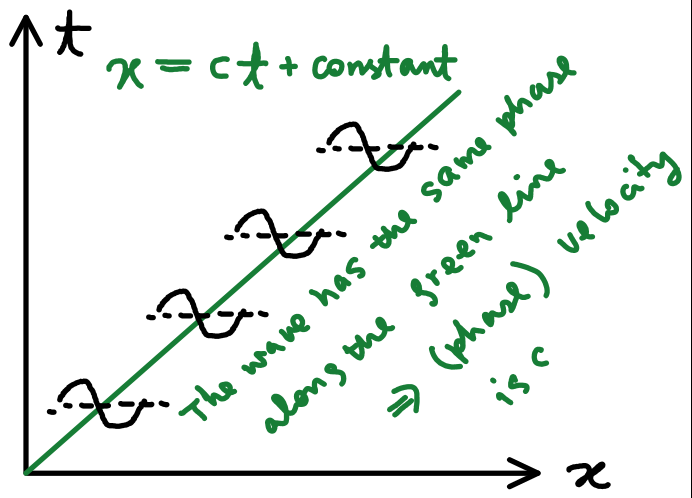
\includegraphics[width=\textwidth, trim={0 2pt 2pt 0}, clip]{phase_velocity}
		\\
	我们将在本课程后面的量子力学中遇到类似的波动方程,并使用复数解 $\exp[ik(x-ct)]$。 因此,一定要明白为什么 \eqref{eq:maxwell_wave} 描述的是一个移动的波。
		\mnewline
如果从更深层次思考,上述相速度实际上并不是描述信息传播速度的方式。 然后我们需要更谨慎地求解麦克斯韦方程组,并找到一个由加速源产生的解,然而这超出了当前讨论的范围。}
	因此, 左边=右边是一个波动方程:
	\begin{align}
		\label{eq:maxwell_wave}
		\frac{\partial^2}{\partial t^2} \mathbf{B} 
		- \frac{1}{\mu_0\epsilon_0} \nabla^2 \mathbf{B} = 0~. 
	\end{align}
	
	
	在数学物理方法的课程中, 我们会研究如何系统地求解这个方程。 但在这里我们不会这样做,相反的,我们可以给出一个解并检查它是否确实满足了 Eq.~\eqref{eq:maxwell_wave} 而无需运用更多数学知识。 我们可以检查一下以下的电磁 波是否是方程的解:
	\begin{align}
		\label{eq:sol_maxwell_wave}	B_z = B_0 \cos [k (x - ct) ]~,
		\qquad \mbox{where~} c \equiv \frac{1}{\sqrt{\mu_0\epsilon_0}} ~.
	\end{align}
计算得出的结论是:一旦发射一束电磁波,它就可以在真空中传播而无需发射器的参考,即发射器的运动信息被“遗忘”。 光速由自然常数 $\mu_0$ 和 $\epsilon_0$ 计算,与发射器(或观察者)的速度无关。 因此我们得出结论,答案是 $c_3=c$,与王二观察到的速度相同(即 $c_3=c_2$)!}

此刻一定有什么大错特错了:速度相加规则\eqref{eq:vel_add_newton}与独立于观察者的光速\eqref{eq:sol_maxwell_wave}不一致。 在这种情况下,我们需要通过实验来判断谁是对的。 迈克尔逊-莫雷干涉仪实验(1887 年)表明麦克斯韦是正确的。 牛顿力学的速度相加法则不适用于光!
\needspace{.1\textheight}
\mtextbox{近代的干涉仪}{
迈克尔逊-莫雷干涉仪旨在测量光速的变化。现在我们知道(至少可以假设)光速确实是一个常数,一个干涉仪可以通过调节干涉臂长度来实现精确测量。它在近代物理和近代计量技术中都有着重要的应用。}

\textbox{迈克尔逊-莫雷实验}{\index{迈克尔逊-莫雷干涉仪}
	\begin{minipage}
		{0.45\textwidth}
		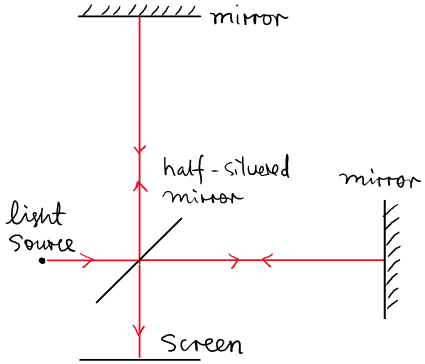
\includegraphics[width=\textwidth]{mm-experiment}
	\end{minipage}\hspace{0.04\textwidth}
	\begin{minipage}
		{0.5\textwidth} 一束光从光源发出,通过半镀银镜(分光镜),光束被分成两束,分别被两个镜子反射到屏幕上。由于光程不同,会产生干涉条纹。
		
请注意,该实验是在地球上进行的。 地球以 $v\sim 30 $km/s 的速度围绕太阳运动。 因此,如果牛顿力学的速度相加规则适用,迈克尔逊-莫雷干涉仪中的光速应该随着旋转而变化,然后干涉条纹应该移动。 但是没有观察到这种变换,因此速度没有增加。 因此麦克斯韦的理论战胜了牛顿的理论。	\end{minipage}
}

\mtextbox{是牛顿错了吗?}{
既然速度加法(在牛顿力学的核心)对光无效,牛顿错了吗? 我们应该放弃牛顿力学吗?	\mnewline
在现代物理学中,我们认为大多数理论都是“有效的”理论——它们适用于某些近似值。 当 $v\ll c$ 时,牛顿力学仍然有用,因为它非常精确,而且比狭义相对论更简单、更直观。	\mnewline
因此,学习狭义相对论并不是要我们要放弃牛顿力学。 相反,在现代,牛顿力学仍然比狭义相对论使用的更广泛(因为我们通常不以 $v\sim c$ 移动或考虑受 $v/c$ 影响的修正)。
\mnewline
事实上,狭义相对论也有类似的命运——它是经典的。 当考虑非常小的粒子时,必须考虑量子力学,我们得出了量子场论。 而考虑到引力的量子效应,量子场论又是远远不够的……}
\textbox{选读的历史内容: 以太的故事}{\index{aether}
	事实上,我们在这里介绍的不是研究人员在 100 年前做出这些发现时的想法。

在麦克斯韦时代,人们认为电磁波在称为以太的介质中传播,类似于在空气中传播的声波。 因此,光速 $c=1/\sqrt{\mu_0\epsilon_0}$ 也是相对于以太而言。 参数 $\mu_0$ 和 $\epsilon_0$ 被认为是以太的属性,而不是真空的属性。	
既然如此,速度相加规则就没有问题了——就像风的速度和声波在风中传播的速度相加一样。
现在的问题是:当地球绕太阳公转时,地球周围的以太是与地球一起运动的,还是保持静止的?
对恒星畸变(1600s - 1700s)的观察表明,以太不与地球一起运动。 在以太的背景下,迈克尔逊-莫雷实验表明以太确实与地球一起移动。 这是100年前困扰物理学家的问题。 而爱因斯坦的贡献是用他的相对论消除了对以太的需要。
由于以太的理论被废弃,现在我们学习电磁波时,我们不再介绍以太,我们选择用更接近现代思维的介绍方式,而不是历史思维,因此我们只在这个这里留下一个关于以太的评论。}

\subsection{爱因斯坦的相对论}

我们如何化解麦克斯韦独立于观察者的$c$与速度加法规则之间的矛盾呢? 这是20世纪初物理学的两大难题之一。 

爱因斯坦 16 岁时,就已经对光产生了深深的困惑:如果我跑得像光一样快怎么办? 光会静止吗? 10年后,他找到了解决办法。

以下是爱因斯坦在 1905 年解决这个问题的方法:他将 $c$ 相对于观察者的独立性作为他理论的基本假设。于是问题解决了:
)

每个人都可以做出假设,但真正具有革命性的是假设的含义以及如何在此基础上获得统一的理论。为了更清晰的理解爱因斯坦的理论,我们在这里总结了假设,并进行更深入的研究。
 
\mtextbox{Remarks about ($\mathbb{C}$)}{
	\mtitem{
		\item 光的速率与观察者无关,但并不是说与速度无关。换句话说,光的方向可以取决于观察者。稍后我们将在讲到“光钟”时清楚地看到这一点。

		\item 光的频率取决于观察者(相对论多普勒效应)。当你向光移动时,光频率会变高(蓝移)。当你远离光时,光频率变低(红移)。

		\item 在非真空情况下,光速将取决于介质的运动。稍后可以使用相对论速度相加规则来获得介质中移动坐标系的光速。
 
	}
}
\itembox{狭义相对论的基本假设}{}{\index{狭义相对论的基本假设}
	\item ($\mathbb{R}$) 相对性原理:物理定律在所有惯性系中都是相同的。

	\item ($\mathbb{C}$) 在在所有惯性系中,真空光速为 $c$。

} 

 ($\mathbb{R}$) 和 ($\mathbb{C}$)是狭义相对论中的基本假设。但要明确的是,还必须假设事件观察者的独立性才能满足狭义相对论理论的基本要求:


\textbox{独立于观察者的事件假设}{\index{事件}
	($\mathbb{E}$) 
	让我们考虑一个在特定时刻发生在一个特定小物体上的事件 (在时空坐标中确定的一点),事件发生(或不发生)与观察者无关。如果一个观察者发现事件 E 发生了,那么所有看到该事件的观察者都必须观察到(同意)此事件发生了,无论他们是如何移动的。

	
	\tcblower
	
	尽管这个假设看起来非常的微不足道,但还是让我们把事情说清楚。

例如,以下是所有(诚实的)观察者必须同意的事件:

	\titem{
		\item ``一束光被镜子反射''
		\item ``王一和王二见面了。见面的时候,他们的手表都指向了上午10点。''
	}
以下这些就不是事件:
	\mtextbox{不是一个事件,而是两个事件的情况}{在王二和王三相隔5光年的例子中,这句话不是一个事件,但可以把它分成两个事件:当王二看她的手表时,她的手表显示上午10点。当王三看他的手表时,他的手表显示的是上午10点。这同样适用于标尺示例的比较。讨论相对论中事件的关系是有道理的,我们将在后面看到。}
	\titem{
		\item ``王二和王三相距5 光年。当王二的手表指向上午 10 点时,王三的手表也指向了上午 10 点。''
	}
这不是事件,因为 Alice 和 Bob 在不同的位置。因此,观察者查理可能会认为上述陈述是正确的;而另一个运动的观察者却认为上述说法是错误的。

同样,以下内容也不是事件,或许所有的观察者都不认可这种陈述:
	\titem{
		\item ``移动的尺子与静态的尺子具有相同的长度,因为两个端点同时重合。''
	}
}

\textbox{注:事件相对于某个参考系发生的时间}{
由于光速有限,我们需要讲清楚事件发生的时间。例如,事件发生在距离鲍勃一定距离的地方。在谈到事件的时间时,它可以指:

	\marginnote{
		我们说在每一个空间点上的钟指的是: 钟相对于bob静止并且和bob的坐标系是完全同步的, (他坐标系中的时间). 同步时钟可以通过比较光信号, 并减去用于光传播的时间来完成。
		\\
		“观察”或者“记录”的意思是假设 Bob在他的参考系中的每个点都有一个助手。一旦发生任何事件,助手可以立即记下 Bob 的时间和事件的空间坐标。这将由事件 $(t_B, x_B)$相对于Bob的坐标表示。}
	\titem{ 
		\item Bob 参考系中的时间。想象一下,鲍勃在他的框架中的每个空间点都放了一个时钟,它“观察”到了事件发生的时间。

		\item Bob 实际“看到”事件的时间。这需要占用事件和 Bob 之间的光传播时间。
	}
	在本课程中,当谈论 Bob 的时间时,除非另外强调,否则我们将默认使用 Bob 参考系中的时间,而不是 Bob 实际看到到达他的事件的光信号的时间。

}

有了这三个假设,我们现在准备开始狭义相对论的旅程。


\section{时间膨胀(钟慢效应)}\label{sec:time-dilation}

    在这部分的开头,我们承诺了读者会在后文解释为什么太空旅行者爱丽丝回来时比鲍勃年轻(如果她在太空旅行前最初与鲍勃年龄相同)。探寻清楚这个问题这就是本节的目标。

    为此,我们必须提及到物理学中最基本的概念——时间。首先,让我们回顾一下牛顿是如何评论时间的。

\mtextbox{我们可以相信的什么?}{
    现在我们要超越牛顿,你可能想知道,我们能相信牛顿理论的什么。我们当然想站在牛顿的肩膀上把他的一些遗产物尽其用。
	\tcblower
    几乎所有低速运动($v\ll c$),牛顿力学的结果都是可信的(除了静止能量,我们将在后面讨论)。对于高速运动 ($v\sim c$),我们只相信 $(\mathbb R)$、$(\mathbb C)$、$(\mathbb E)$ 。
    \mnewline
    例如,在讨论时间时:我们相信爱丽丝的机械表(静态的爱丽丝)很好地定义了爱丽丝的时间,因为机械表的时间是低速机械运动的结果。但是我们不能相信牛顿理论中关于爱丽丝的时间(由她的机械表的转动来定义)如何在鲍勃身上流逝的结论,如果鲍勃相对于爱丽丝有 $v\sim c$ 的相对运动。在讨论长度时:我们相信爱丽丝的尺子(静态的爱丽丝)定义了爱丽丝的长度,但我们不能相信鲍勃如何观察爱丽丝的尺子的长度。
}
\textbox{牛顿理论中的时间}{\index{牛顿理论中的时间}
	``绝对的、真实的和数学的时间,它本身,从它的本性出发,平等地流动,不考虑任何外部的东西,另外一个名字叫做持续时间:相对的、明显的和普通的时间,是一些合理的和外部的(无论是准确的还是不公平的) ) 通过运动来测量持续时间,通常用于代替真实时间'' 
	-- 牛顿《自然哲学的数学原理》
	
	\tcblower

    因此,牛顿相信“真实时间”独立于任何其他事物而存在。如果是这样,怎样才可以测量真实时间呢?

	\titem{
		\item 如果我们无法得到它, 那我们为什么要耗费精力去定义“真实时间”呢? 我们为什么不直接摒弃这个概念呢?
		\item 如果它可以被一个设备测量出来,那为什么它不能被这个设备改变呢?我们想一想牛顿第三定律,当真实时间对装置产生某种作用时,为什么装置不能对真实时间进行反向的作用并改变它呢?
    }
}

我们是物理学家。我们可以做些什么来摆脱关于时间的形而上学思维呢?我们来做一件实际的事情——通过实际制作一个最简单的时钟来定义时间:光钟。

\textbox{制作光钟}{\index{光钟}
	\begin{minipage}
		{0.45\textwidth}
		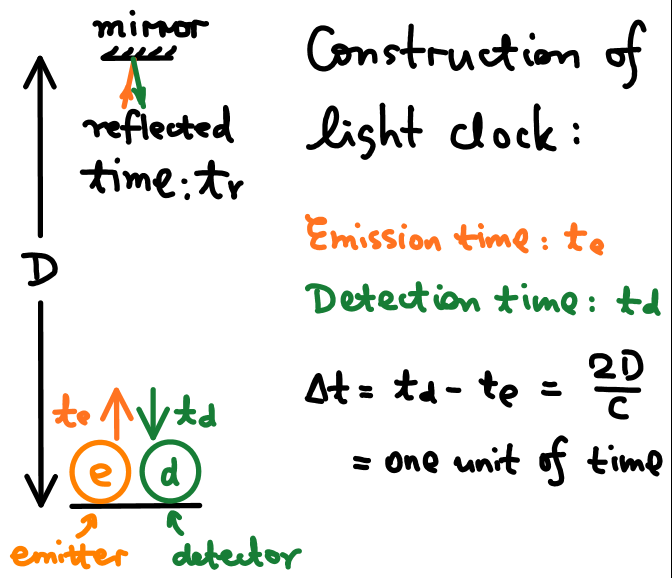
\includegraphics[width=\textwidth, trim={0 3pt 3pt 0}, clip]{light_clock}
	\end{minipage}\hspace{0.04\textwidth}
	\begin{minipage}
		{0.51\textwidth}我们用光钟的滴答声来定义时间间隔。 滴答时间间隔 $\Delta t$ 是发射器发射光(时间 $t_e$)和检测器检测到光(时间 $t_d$)之间的时间。在过程中,光被镜子反射(在时间 $t_r$)。
对于光钟,“标准时间间隔”可以定义为 \marginnote{发射器和检测器放在一起,它们非常接近,我们可以认为在同一点上(在图中它们分开绘制只是为了表示清楚)。}
		\begin{align}
			\label{eq:time_interval}
			\Delta t \equiv t_d - t_e = \frac{2D}{c}~. 
		\end{align}

		于是我们就可以通过两个事件之间的“标准时间间隔”的数量来测量时间了。
	\end{minipage}
}

为了了解旅行者的时间相比于静态观察者如何,我们把光钟放到爱丽丝的车上。

\textbox{把光钟放到爱丽丝的车上}{
	\begin{minipage} 
		{0.6\textwidth}
		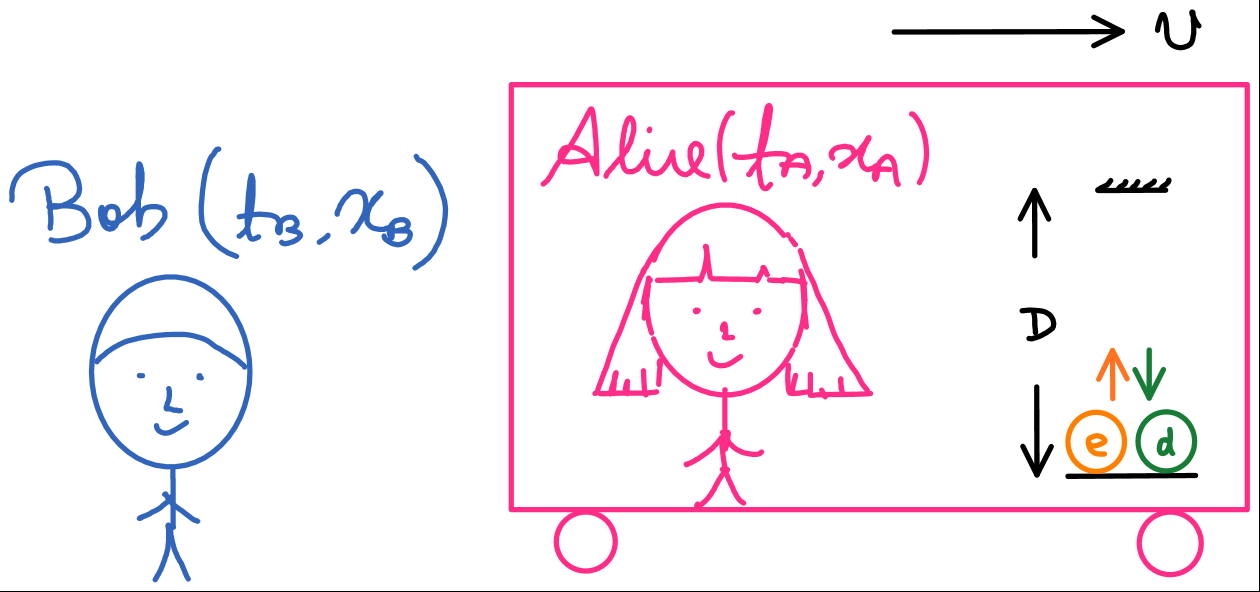
\includegraphics[width=\textwidth, trim={0 3pt 3pt 0}, clip]{light_clock_car}
	\end{minipage}\hspace{0.04\textwidth}
	\begin{minipage}
		{0.36\textwidth} 
		To 
		\marginnote{这里我们假设光钟离爱丽丝足够近,在爱丽丝的参考下,她自己和时钟的空间坐标都是 $x_A=0$。}
        现在让我们与爱丽丝一起将光钟装入汽车,看看旅行者的时间流逝与静态观察者相比如何。根据 ($\mathbb{R}$),Alice 发现光钟的间隔是 $\Delta t_A = 2D/c$。

现在我们需要找出 $\Delta t_B$ 并将其与 $\Delta t_A$ 进行比较。
	\end{minipage}	
}

\needspace{.25\textheight}
\mtextbox{相同的垂直长度}{
	此时你可能有一个很好的问题:当光钟在移动时,我们怎么知道光钟的长度相比于Bob仍然是 $D$ ?

	\tcblower
	考虑一个思想实验:火车在轨道上。列车静止时,其车轮的间距与轨道宽度相同。现在火车开得很快。与轨道相比,它的轮子的宽度是更大还是更小?两者都不。否则就会发生与 ($\mathbb{E}$) 矛盾的事故。

}
\textbox{鲍勃测量的爱丽丝光钟的时间间隔}{
	\begin{minipage}
		{0.55\textwidth}
		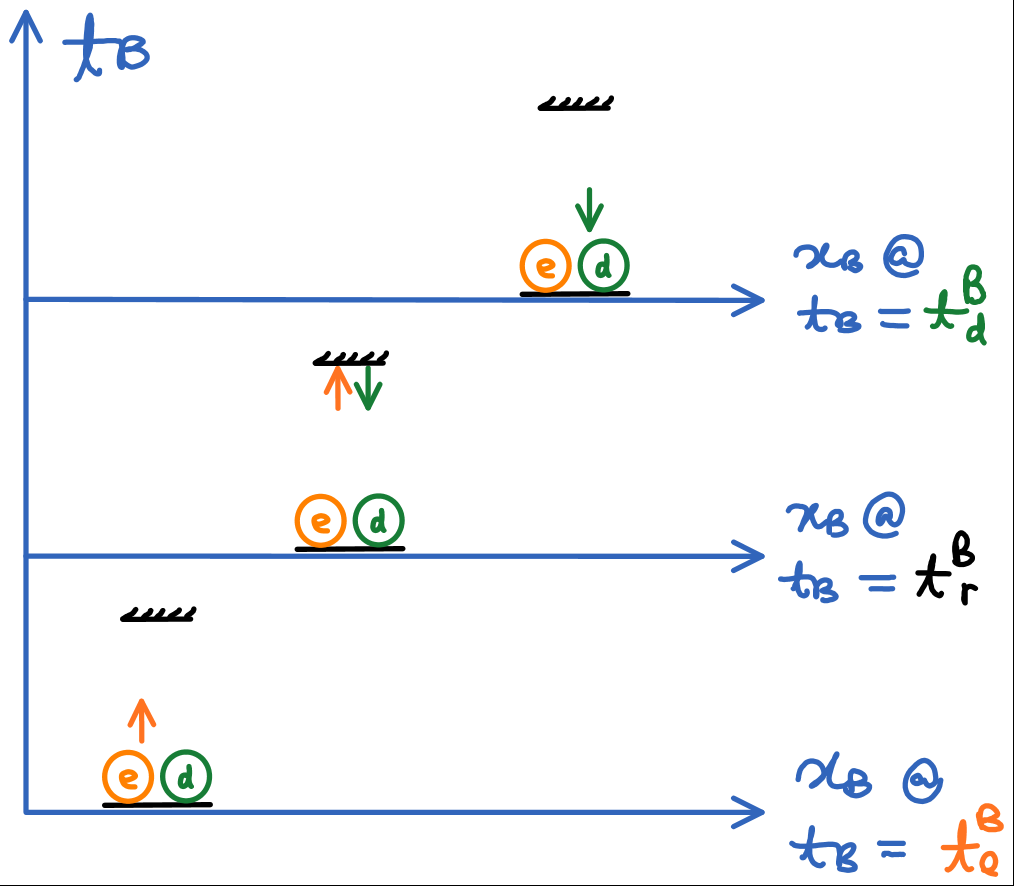
\includegraphics[width=\textwidth, trim={0 2pt 2pt 0}, clip]{light_clock_B}
	\end{minipage}
	\hspace{0.05\textwidth}
	\begin{minipage}
		{0.4\textwidth}
		左图是鲍勃对移动时钟的看法。这里 $x_B$ 和 $t_B$ 分别是鲍勃的空间和时间。
		
		我们拍摄了三个时间快照:在 $t_B = t_d^B$ 处的信号发射,光被镜子反射的时间 $t_B = t_r^B$,以及光被接收器接收的时间 $ t_B=t_d^B$。

        光钟的位置和状态如图。
	\end{minipage}

	\bigskip

	\begin{minipage}
		{0.35\textwidth}
		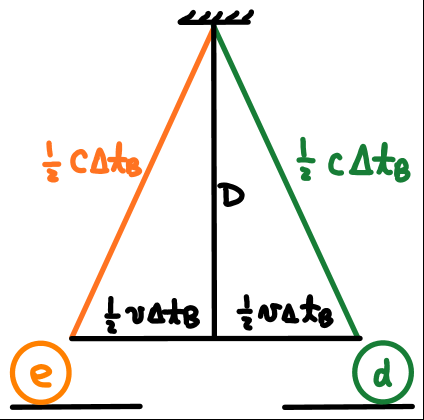
\includegraphics[width=\textwidth, trim={0 2pt 2pt 0}, clip]{light_clock_B1}
	\end{minipage}
	\hspace{0.05\textwidth}
	\begin{minipage}
		{0.6\textwidth}
		在左图中,我们绘制了 Bob 的移动光钟中的光轨迹。鲍勃一定认可光线击中了镜子 ($\mathbb{E}$)。因此光的方向必须不再是垂直的。并且从($\mathbb{C}$),从发射器到镜子的光速仍然是$c$。

		
		根据勾股定理,我们有
		\begin{align}
			\label{eq:lcb}
			\left ( \frac{1}{2} c \Delta t_B \right )^2 = \left ( \frac{1}{2} v \Delta t_B \right )^2 + D^2 ~,
		\end{align}
	\end{minipage}

	\bigskip

	\tcblower
	
	因此,我们可以求解 $\Delta t_B$ -- Bob测量的Alice的时间间隔:

	\begin{align}
		\label{eq:dtb}
		\Delta t_B = \frac{2D}{c} \frac{1}{\sqrt{1-\frac{v^2}{c^2} }} = \gamma \Delta t_A ~,
		\qquad
		\gamma \equiv \frac{1}{\sqrt{1-\frac{v^2}{c^2} }} > 1~.
	\end{align}
	因此,在王三的参考系中,王二的光钟变慢了。这也被称为移动时钟的“时间膨胀”(也就是动钟变慢)。
}

\textbox{不仅是王二的光钟,整个王二参考系相对于王三都变慢了
}{
	在这时, 
	\marginnote{``你的钟如何与我无关。我在乎的是你呀。'' -- 王三}
	我们说王二的一切相对于王三都减慢了是不够有说服力的。 因为我们只是说明了她的光钟变慢了。 那么她的闹钟,手机,心率又是怎么样的呢?

	\mtextbox{和绝对时间说再见吧}{通过“动钟变慢”,人们注意到牛顿的“绝对时间”概念随着速度而消失。 不同的搬运工有不同的时间; 没有绝对的推动者,因此也没有绝对的时间。
	\\
	我们在稍后以及在学习到广义相对论章节时还会回到}

	\tcblower

	事实上,根据 ($\mathbb{R}$),上述的一切都变慢了。

	假如 Alice 有一个手机,它可以定义单位时间间隔。 她把光钟和手机放在非常靠近的地方。 如果手机和光钟在静止参考系中具有相同的 $\Delta t$,则它们必须具有与 Alice ($\mathbb{R}$) 相同的 $\Delta t_A$。 他们的共识是一个事件,Bob 必须同意 ($\mathbb{E}$)。 因此鲍勃必须同意手机与光时钟定义的 $\Delta t_B$ 是相同的。
}

\textbox{狭义相对论中的总结和四步推理}{\index{时间膨胀}\index{四步推理}
	我希望现在你已经明白为什么太空旅行者爱丽丝回来时比鲍勃年轻——作为一个移动的观察者,她相对于鲍勃变慢了。

	\mtextbox{ $\Delta t_B$的意义}{这里注意,$\Delta t_B$ 并不是 Bob 光钟的时间间隔,而是 Alice 的光钟(即与 Alice 一起移动)在 Bob 的参考系中的时间间隔。 所以说相对于鲍勃(静态观察者),爱丽丝的时间变慢了。}
	\tcblower

	推理的4个关键步骤很重要,我们将重复使用类似的方法。 因此,让我们在这里总结一下:
	\tenum{
		\item 在静静止参考系中构建仪器。 仪器应该尽可能简单,以便我们计算仪器内部实际发生的情况。 这里的装置是标准时间间隔$\Delta t = 2D/c$的光钟。
		\item 将装置放入爱丽丝的移动汽车。 根据 ($\mathbb{R}$) ,Alice的观察结果一定是设备运动与静止时的工作方式是相同的。 这里 Alice 发现 $\Delta t_A = \Delta t$。
		\item 计算鲍勃得到的结果,将结果与 Alice 得到的结果进行比较。 我们已经计算出 $\Delta t_B = \gamma \Delta t_A$。 因此,移动的光钟变慢了。
		\item 虽然结果是由一个特定的仪器获得的,但 Bob 的参考系和 Alice 的参考系之间的比较适用于所有的设备。 因为要不是这样,就可以使用这个差异来识别绝对运动的人了 ($\mathbb{R}$)。
	}
}

\textbox{参考系的时间以及Bob看到了什么}{
	\twocol{0.85}{0}{0.65}{
		我们已经提到了“参考系的时间”这个概念:如果没有另外说明,当我们提到时间时,我们指的是一个人参考系中的时间,而不是光进入观察者眼睛的时间。 现在让我们更清楚地说明这一点。

让我们在空间中的每个点(比如 $x$-方向)放置两个东西:
		\titem{
			\item 一个空间标记。 例如,假设沿 $x$ 方向有一个标尺,标尺的刻度就是空间标记。
			\item 一个钟。时钟在空间中的所有点都是同步的(有关如何同步时钟的信息,请参阅关于校对时钟的部分)。 
		}
		时间膨胀 ($\Delta t_B$) 的意思是,Alice 的时钟(标有 $\vec v$ 的红色时钟)在移动,下一时刻,它与 Bob 参考系中的另一个时钟进行比较,并且它变慢了。在这个比较中,时间膨胀不取决于爱丽丝的车是向鲍勃运动还是远离鲍勃运动。

		Bob 实际“看到”的东西,用 $\Delta t_B^{\mbox{``see''}}$ 表示:由于光速是有限的,所以光会有延迟。光线从 Alice 的时钟传播到 Bob 的眼睛(红色波浪线)。 $\Delta t_B^{\mbox{``see''}}$ 取决于爱丽丝是向鲍勃运动还是远离鲍勃运动。
	}{
		\cg{0.9}{frame_meaning}
	}	
}

    既然你已经了解了时间膨胀以及为什么太空旅行者爱丽丝更年轻。 那么现在就是再次把你搞糊涂你的好时机,让我们来看看著名的“双生子佯谬”。

\needspace{0.4\textwidth}
\mtextbox{时空旅行?}{
	双生子佯谬是时间旅行到未来的一个例子。 如果你乘坐宇宙飞船旅行并返回,你就会到达未来。 如果太空旅行足够快,往返在1年之内,你就可以看到下个世纪,甚至更晚的地球。 在广义相对论中,我们将看到更多前往未来的方式,例如靠近黑洞。
	\mnewline
	穿越到过去呢? 一会我们就会发现狭义相对论是如何防止通过时间旅行回到过去的。 还有比较普遍的问题,比如穿越到过去,不让爸爸妈妈见面会怎么样? 如果你穿越到过去,遇到另一个自己怎么办?  穿越到过去大概是不可能的,虽然此刻我们还无法做出决定性的结论。
}
\textbox{谁在运动?到底谁更年轻呢? -- 双生子佯谬}{\index{双生子佯谬}
	我们已经证明:Bob 发现 Alice 更年轻(根据他参考系中的时钟)。 然而,运动是相对的($\mathbb{R}$)。 因此,爱丽丝不也应该发现鲍勃更年轻吗?

	\tcblower

	让我们通过两个步骤来解决这个问题:
	\tenum{
		\item Alice 和Bob的参考系都是惯性系,它们一直有相对运动。 根据 ($\mathbb{R}$),“Alice 认为 Bob 更年轻”和“Bob 认为 Alice 更年轻”都是正确的。

		乍一看,这与 ($\mathbb{E}$) 矛盾,但实际上并不矛盾。 作为匀速运动的人,爱丽丝和鲍勃只能见面一次。 这是一开始 Alice 与 Bob 年龄相同的时间,后来他们再也没有见面。 因此,没有本地事件来比较他们的年龄(使用 \emph{events} 比较 $\Delta t_B$ 和 $\Delta t_A$,它们必须至少相遇两次)。

		\item 爱丽丝先运动,然后折反回来见到鲍勃。 这与我们在本部分的开始讨论的设置相同。

		我们目前只能相信鲍勃。这是因为Alice要折返,这段时间Alice不在惯性系中。 相对性原理(我们在得出结论时使用了很多次)不适用于非惯性观察者。 因此,我们只能相信 Bob 的观点,即 Alice 更年轻。
	}
}

\section{物理图像和物理直觉}\label{sec:phys-pict}

本节无关物理的理论知识。考虑到现代物理学与经典物理学如此不同,停下来讨论学习方法是很重要的。  我们选择把这个部分放在这里而不是最开始(尽管这在逻辑上更合理),是因为在没有任何现代物理的实际经验之前,谈论这些是空洞的。

\textbox{为什么现代物理不同于经典物理(即普通物理)?}{
	从狭义相对论的时间膨胀,你已经初步接触了现代物理学的一点理论。 如果你还没有学过它,你一定会觉得它是违反直觉的,比普通物理的绝大多数部分更令人困惑。

	之后还要更多现代物理的理论——你将了解更多关于相对论、引力、量子、信息、复杂性的知识……面前是一个全新的世界。 这些主题的共同特点不仅是它们是在大约过去100年才被发现的,而且它们离我们的日常经验更远。 这就与是经典物理学的不同之处。

	不要被这些吓到!这就是这一节存在的原因。

	\tcblower

	顺便说一下,数学、文学和艺术也有类似的过渡——它们也从古典演变到现代。 文学、艺术、数学和物理的现代化革命固然不同,但有着有趣的相似之处。
}

让我们用一个练习来谈谈思考的方法,以及学习现代物理值得推荐的方法。

\textbox{小练习}{
	一枚“手榴弹”
     \marginnote{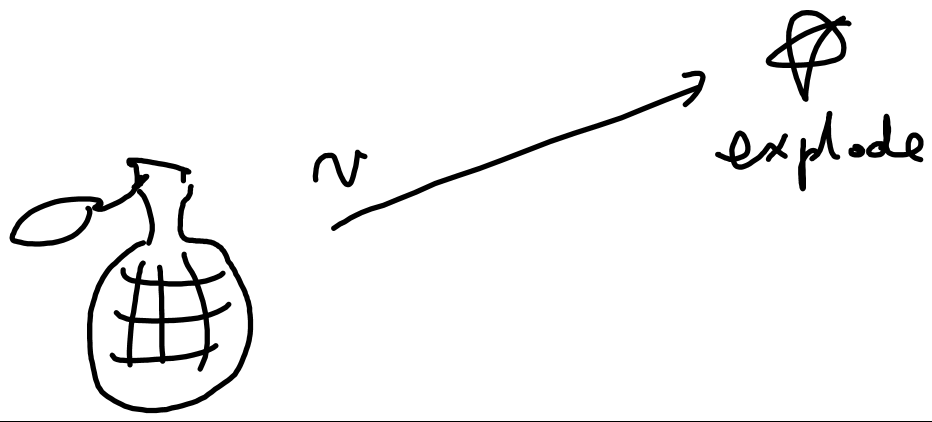
\includegraphics[width=0.3\textwidth, trim={0 2pt 2pt 0}, clip]{grenade}}
是一种在触发后一定时间爆炸的炸弹。 设手榴弹静止时触发到爆炸的时间间隔为$\Delta t$。 现在你以 $v$ 的速度扔手榴弹。 计算狭义相对论理论下手榴弹爆炸前运动的距离。 在计算中,地球重力和空气摩擦都可以忽略。
	
	\tcblower

	在解决这个问题之前,让我们讨论 3 种“思考”如何解决它的方法(\emph{不是} 三种解决方法)。

	\titem{
		\item \emph{配对}。 将问题配对(转换)为已解决的问题: "Bob" $\leftrightarrow$ "你"; "爱丽丝" $\leftrightarrow$ "手榴弹"; $\Delta t_A$ $\leftrightarrow$ $\Delta t$ 因此$v\Delta t_B = \gamma v \Delta t$ $\rightarrow$ $s$。
        \item \emph{反向推理}。 问距离,那么如何计算距离,速度给定,所以$s=v t$。 现在如何得到$t$? 哪个方程有 $t$? 这是一个关于相对论的问题,所以应该是 $\Delta t_B = \gamma \Delta t_A$(希望你得到 $\gamma$ 而不是 $1/\gamma$)。 因此,$s=\gamma v \Delta t$。
        \item \emph{实物图像}。 想象一下手榴弹飞出一段距离然后爆炸。 你看到了文字,但在你的脑海中播放了一段画面。 手榴弹的时间变慢了。 所以它必须比平时运行更长的时间,从而运行更长的距离。 飞行时间长了一个 $\gamma$ 因子,因此行进的距离长了一个 $\gamma$ 因子:$s = \gamma v \Delta t$。
	}
}

在准备考试时,我们可能主要使用第一种和第二种方法进行了大量培训。 但如果你想成为一名创新的物理学家,或者至少想成为一名物理学家,那么第三种思维方式是主要的方式。因为:

\itembox{为什么物理直觉和物理图像很重要}{}{
	\item 一张真实的图片可以将你学到的东西与现实世界联系起来,而其他两种方法不可以。在研究中,您需要了解该理论的可能应用,或者如何进行近似以简化分析。实物图片指导您做到这一点,而其他两个方法没有。 
\item 一张实物图片告诉你你的答案是否有意义。如果你在某个地方犯了错误,而你脑子里有一张实物图,那么你就有很好的机会尽早发现它。
\item 研究意味着模式匹配不会给你带来好的结果的新问题。 (但您确实必须使用模式匹配来确保您的想法是新的。)
\item 研究人员必须在解决问题之前定义问题(与已经明确定义的考试问题不同)。清晰的实物图片告诉您如何定义问题。反向搜索或模式匹配不能。
\item 作为一名研究人员,需要与人交谈。在大多数讨论中(尤其是那些没有黑板的讨论),你都是通过实物图片来说话的。
\item 计算机擅长模式匹配和反向搜索。人工智能的兴起更有可能降低你的模式匹配和逆向搜索工作的价值,但不太可能是基于直觉的工作。
}

我希望你现在确信:即使是物理学在现代也变得不那么直观了,你应该尝试通过建立物理图片来使其尽可能直观。这里有一些关于如何实现这一目标的建议。

\itembox{如何在现代物理学中建立物理图像/直觉?}{}{
\item 试着在你的脑海中“播放一部电影”来解决这个问题。在影片中包含尽可能多的相关物理细节。当你对某件事有新的理解时,把它加到“电影”中。
\item 当你发现一些不直观的东西时,请反复思考。你最终会对此感到更快乐。
\item 注意物理学中的悖论,以及它们是如何解决的。
\item 以不同的方式/角度思考同一个问题。
\item 与我们的日常生活经验进行比较。找出相似之处和/或关键差异。
\item 简化和模块化问题。建立对最简单问题的直觉作为更复杂问题的构建块。
\item 如果仍有部分无法使其直观,请暂时使用一些(尽可能少的)数学推导。稍后尝试用真实的直觉替换它。
}

\section{尺缩效应}\label{sec:length}

我们刚刚见证了时间概念的革命——持续时间是相对的,取决于观察者的运动。 那么空间呢? 它仍然是绝对的,还是像时间一样是相对的、取决于观察者的呢?
在本节中,我们将通过 2 种方式得出相同的长度收缩结论。 第一种方式是必须要理解的,而第二种方式则不是必须理解的。但从不同的角度理解相同问题是值得推荐的做法。
\marginnote{事实上,在狭义相对论之前,长度收缩是由斐兹杰惹 (1889) 和 洛伦兹 (1892) 假设的,以解释迈克尔逊-莫雷实验。 因此,它也被称为洛伦兹收缩。 但狭义相对论把尺缩效应通过严谨的方式放到了理论物理的背景中。}

\textbox{回顾手榴弹问题}{
让我们从不同的角度考虑手榴弹问题。 回想一下,相对于地面手榴弹已经飞了一段距离 $s = \gamma v \Delta t$。 现在,手榴弹“想”的是什么呢?
	\marginnote{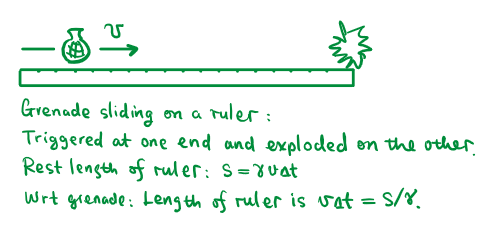
\includegraphics[width=0.35\textwidth]{grenade_length_contraction}}

它仍然有生命周期 $\Delta t$ (相对于它本身)。 虽然它会认为它已经飞了一段距离$v \Delta t = s/\gamma$。 但是站在地面上的观察者认为它已经飞了更长的距离(相对于静态观察者而言)。 怎么会这样呢?

为了让情况更清楚,让我们在地上放一把尺子,让手榴弹滑过尺子。 标尺的剩余长度为 $s = \gamma v \Delta t$。

相对于手榴弹,尺子(和地面)以 $v$ 移动 $\Delta t$长的时间。 因此,尺子相对于手榴弹的长度为 $s/\gamma$。
	\tcblower

总而言之,如果平行于运动方向放置,移动标尺会缩短 $1/\gamma$。 同时回想一下,如果标尺垂直于运动方向,长度不会改变。
}
	

我们会在这里结束该部分的内容。 但是在 $\Delta t$ 时间内手榴弹中发生的事情我们是不知道的。 让我们构建一个光尺来看看究竟发生了什么,这也可以提供有关速度加法的想法。

\textbox{(选读) 光尺的尺缩效应(4步推理)}{\index{运动尺子的}
虽然我们已经得到了结果,但使用另一种方式推导出它是一个很好的做法。 让我们构建一个光尺并研究它是如何收缩的。 这将明确验证我们的承诺:无论标尺如何定义,它都应该以相同的方式收缩。 为了看到这一点,让我们应用我们熟悉的 4 个步骤:
\tenum{
		\item 在静止参考系中,标尺的长度为$D = \frac{1}{2} c \Delta t$,其中$\Delta t$ 是光发射和检测之间的时间间隔。

		\item 现在我们将光尺放到 Alice 的车上。 Bob观察到的情况和时空图如下图所示。

		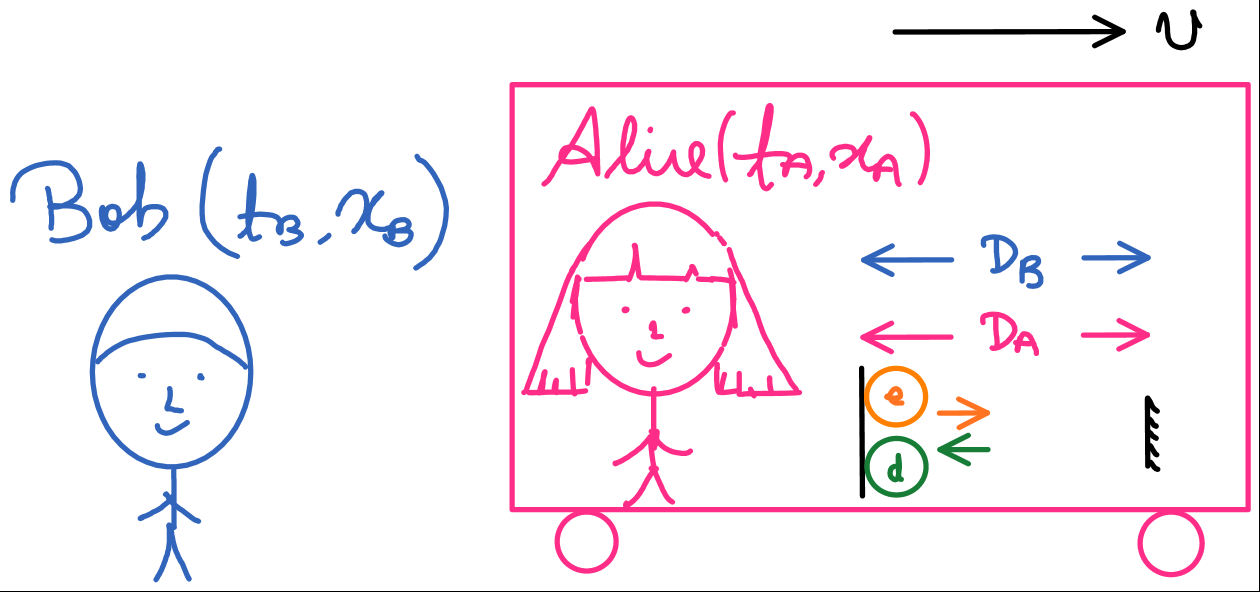
\includegraphics[width=0.5\textwidth, trim={0 3pt 3pt 0}, clip]{light_ruler}
		\hspace{0.1\textwidth}
		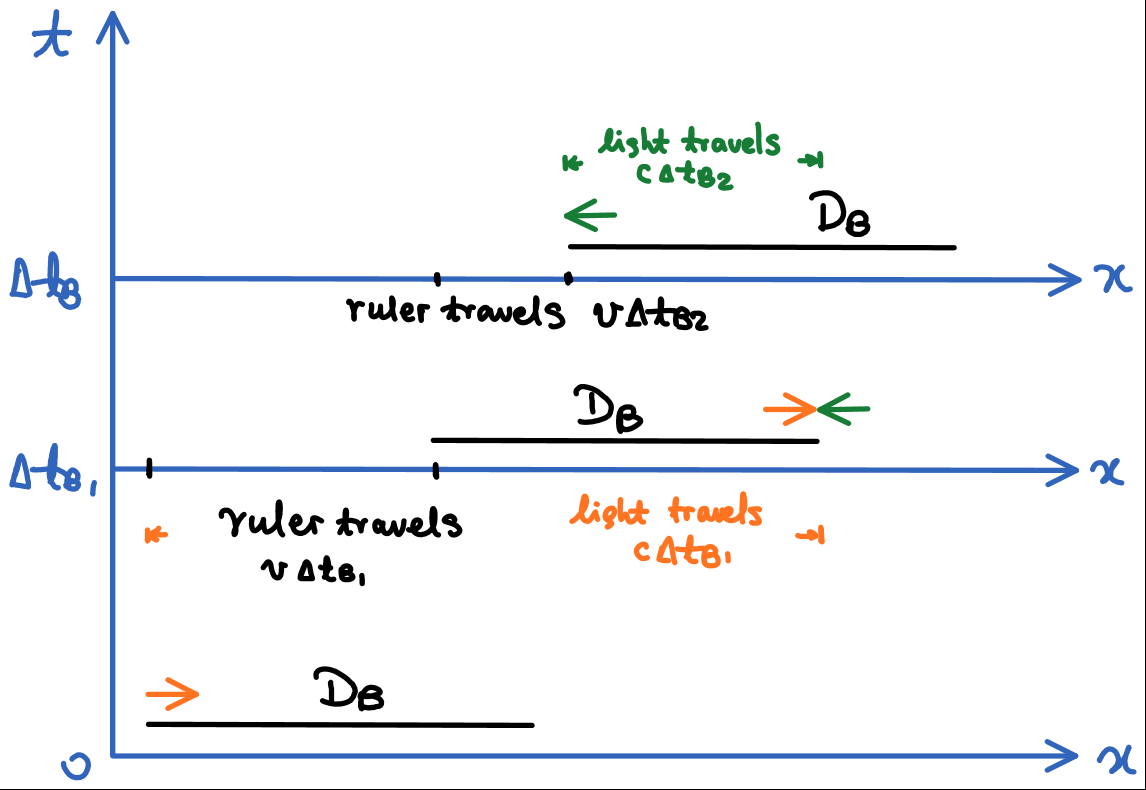
\includegraphics[width=0.6\textwidth, trim={0 2pt 2pt 0}, clip]{light_ruler_2}

		根据 ($\mathbb{R}$),Alice 认为尺子的长度为
		\begin{align}
		\label{eq:ruler_Alice}
		D_A = \frac{1}{2} c \Delta t_A~.
		\end{align}

		\item Bob 应该测量到的长度是多少? 我们首先将时间间隔 $\Delta t_B$ 分为两部分:$\Delta t_{B1}$ 和 $\Delta t_{B2}$ 分别为从发射器到镜子和从镜子到检测器的时间间隔。 从上图(右)可知,
		\begin{align}
		\label{eq:bobx}
		c\Delta t_{B1} = D_B + v \Delta t_{B1}~, \qquad
		c\Delta t_{B2} = D_B - v \Delta t_{B2}~.
		\end{align}
		因此
		\mtextbox{$D_B$ 的含义}{请注意$D_B$ 不是鲍勃尺子的长度。 更确切地说,它是 Bob 参考系中 Alice 的尺子(即与 Alice 一起移动的)的长度。 所以相对于鲍勃(静态观察者),爱丽丝的尺子(移动的尺子)缩短了。}
		\begin{align}
		\label{eq:bobt}
		\Delta t_B \equiv \Delta t_{B1} + \Delta t_{B2} = \frac{D_B}{c-v} + \frac{D_B}{c+v} = \frac{2}{c} \frac{D_B}{1-\frac{v^2}{c^2} }
		= \frac{2}{c} \gamma^2 D_B~,
		\end{align}
		一如既往的, $\gamma\equiv \frac{1}{\sqrt{1-v^2/c^2}} $. Thus
		\begin{align}
		\label{eq:bobalice}
		D_B = \frac{c}{2} \frac{\Delta t_B}{\gamma^2} = \frac{c}{2} \frac{\gamma \Delta t_A}{\gamma^2} 
		= \frac{c}{2} \frac{\Delta t_A}{\gamma} = \frac{D_A}{\gamma}~.    
		\end{align}
		同样,我们得出结论,移动的尺子在运动方向上收缩。

		\item 对于所有的尺子,我们都会得到与光尺一样的结论。
	}	
}

\mtextbox{(选读) 一个速度表}{
	以一种方式将 $c$ 替换为 $v$ 的动机是什么? 我们可以问这个装置在静止时能做什么。 通过$\Delta t = D/u + D/c$,和我们定义的$\Delta t$ 和$D$,我们可以解出$u$。 因此,这个装置是一个速度计。作为一个速度计,也就不难解释为什么它可以告诉我们有关速度加法的信息。
}
\textbox{(选读) 关于速度加法的简单介绍}{\index{速度加法简介}
	让我们稍微修改一下光尺:将来自发射器的光替换为镜像到一个移动的粒子,相对于Alice的速度为 $u_A$  。 在“镜子”接收到粒子之后,“镜子”仍然会发回一束光(因此实际上它不应该被称为镜子)。 那么光尺实验是怎么修改的呢?
	\titem{
		\item 相对于Alice,向前的粒子,$u_A \Delta t_{A1} = D_A$; 对于向后移动的光,$c \Delta t_{A2} = D_A$。 因此,
		\begin{align}\label{eq:fl-veladd1}
			\Delta t_A = \Delta t_{A1} + \Delta t_{A2} 
			= D_A \left( \frac{1}{u_A} + \frac{1}{c}  \right)~.
		\end{align}

		\item 对于 Bob,他会发现粒子以一个不同的速度 $u_B$ 移动。 对于向前运动的粒子,$u_B \Delta t_{B1} = D_B + v \Delta t_{B1}$; 对于向后移动的光,$c\Delta t_{B2} = D_B - v \Delta t_{B2}$。 因此,
		

		\begin{align}\label{eq:fl-veladd2}
			\Delta t_B = \Delta t_{B1} + \Delta t_{B2}
			= D_B \left(  \frac{1}{u_B-v} + \frac{1}{c+v}  \right)~.
		\end{align}
		\mtextbox{(选读) 具有加性的快度}{Eq.~\eqref{eq:add-eg} 看起来很丑。 自然不是更简单吗? 但是谁告诉我们速度是描述运动的最佳变量? 让我们定义 \emph{rapidity}:\label{rapidity} $\phi(v) \equiv \mathrm{arctanh} (v/c)$. 将此定义放到 Eq.~\eqref{eq:add-eg} 中,我们简单地得到
		
		$$ \phi(u_B) = \phi(u_A) + \phi(v)~. $$
		因此快度才是真正具有加性的变量。
		\tcblower
		为什么这里出现双曲函数(它们最初是用加性参数参数化双曲曲线 $x^2-y^2=1$ 的函数,就像三角函数 sin、cos、tan 是参数化圆 $x^2 的函数一样 +y^2=1$ 加角)? 双曲函数是否暗示了一个新的基础数学结构? 为什么这样一个公式中的运动看起来不像是时空的划分,而是时空的双曲线旋转? 我们将在 \ref{sec:geometry} 部分回到这个问题。
		}
		\item 我们已经知道了 $\Delta t_B = \gamma \Delta t_A$ 和 $D_B = D_A/\gamma$. 现在用 \eqref{eq:fl-veladd1} 除以\eqref{eq:fl-veladd2} (LHS and RHS, respectively), 我们得到
		\begin{align} \label{eq:add-eg}
			u_B = \frac{u_A + v}{1+u_A v / c^2} ~. 
		\end{align}
	}
	在我们取 $u_A\rightarrow c$ 的极限的时候, 我们会发现 $u_B\rightarrow c$ 和 $(\mathbb{C})$是一致的。 在 \ref{sec:lorentz}这部分,你会学到速度加法公式更通用的版本。
}

  \textbox{(选读) 两个移动杆的尺缩效应}{
  	爱丽丝和鲍勃分别带着杆并以相对速度 $v$ 朝向彼此移动。 当两杆左端重合时,从杆的左端发出光信号。 当两杆右端重合时,光信号到达棒的右端。

  	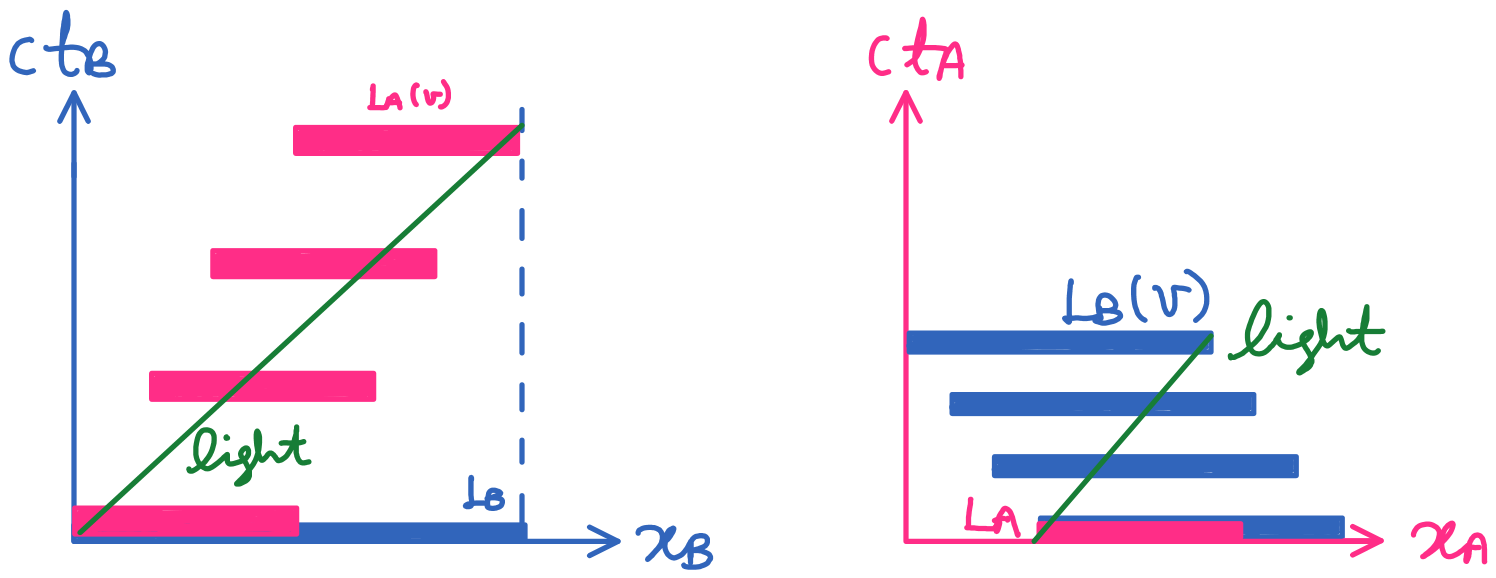
\includegraphics[width=\textwidth]{contraction3}

  	对于上图的情况,根据 Bob(左图):
  	\begin{align}
  	\label{eq:c3bob}
  	\frac{L_B-L_A(v)}{v} = \frac{L_B}{c}~,  \quad\rightarrow\quad
  	\frac{L_A(v)}{L_B} = 1- \frac{v}{c} ~,  
  	\end{align} 
  	根据Alice (右图),
  	\begin{align}
  	\label{eq:c3alice}
  	\frac{L_B(v)-L_A}{v} = \frac{L_A}{c}~,  \quad\rightarrow\quad
  	\frac{L_B(v)}{L_A} = 1+ \frac{v}{c} ~.
  	\end{align}
  	把上述两图相乘,
  	\begin{align}
  	\label{eq:c3m}
  	\frac{L_A(v)}{L_A} \frac{L_B(v)}{L_B} = 1- \frac{v^2}{c^2}~.   
  	\end{align}
  	这种关系适用于所有长度 \marginnote{更改 $L_A$,方程右边的式子不会改变,因此右式不应该依赖于 $L_A$。 出于同样的原因,右式不依赖于 $L_B$}。 结果,我们必须有
  	\begin{align}
  	\label{eq:c3}
  	\frac{L_A(v)}{L_A} = \frac{L_B(v)}{L_B} = \sqrt{1- \frac{v^2}{c^2}} = 1/\gamma~.
  	\end{align}
  }

我们现在从光钟得到了两个结果,第一个是时间膨胀(钟慢)。在已知时间膨胀之后,我们旋转光钟得到长度收缩(尺缩)。在知道了知道长度收缩之后,我们还能得到别的东西吗?

\section{“同一时间”(同时性)的含义} \label{sec:same-time}

我们知道动尺变短。 现在,我们比较两个标尺是否会产生悖论? 如果 Alice 和 Bob 各自拿着一把尺子沿着他们的运动方向,当他们相遇时,他们比较了他们的尺子的长度,他们会发现对方的尺子更短吗? 为什么会这样呢?

关键的问题是是,想要公平,他们必须同时比较标尺的两端。 但是等等,他们有相同的时间概念吗?

\subsection{同时性取决于观察者是谁}

\needspace{0.1\textwidth}
\mtextbox{为什么要引入两个物体?}{需要实际对象 $P$、$Q$ 才能找到站在中点的观察者。 因为中点是为空间中的两个点($P$ 和 $Q$)定义的,而不是为时空中的两个事件($E_P$ 和 $E_Q$)定义的。}
\textbox{相对于观察者同时性的含义}{\index{同时性}\index{相同时间}
	考虑两个小物体 $P$ 和 $Q$,它们之间没有相对运动。
观察者正好站在 $PQ$ 的中点,并且没有相对于 $PQ$ 移动。这实际上可以使用静态标尺完成:让 $P$ 在 0m 处,$Q$ 在 1m 处,观察者在 0.5m 处。

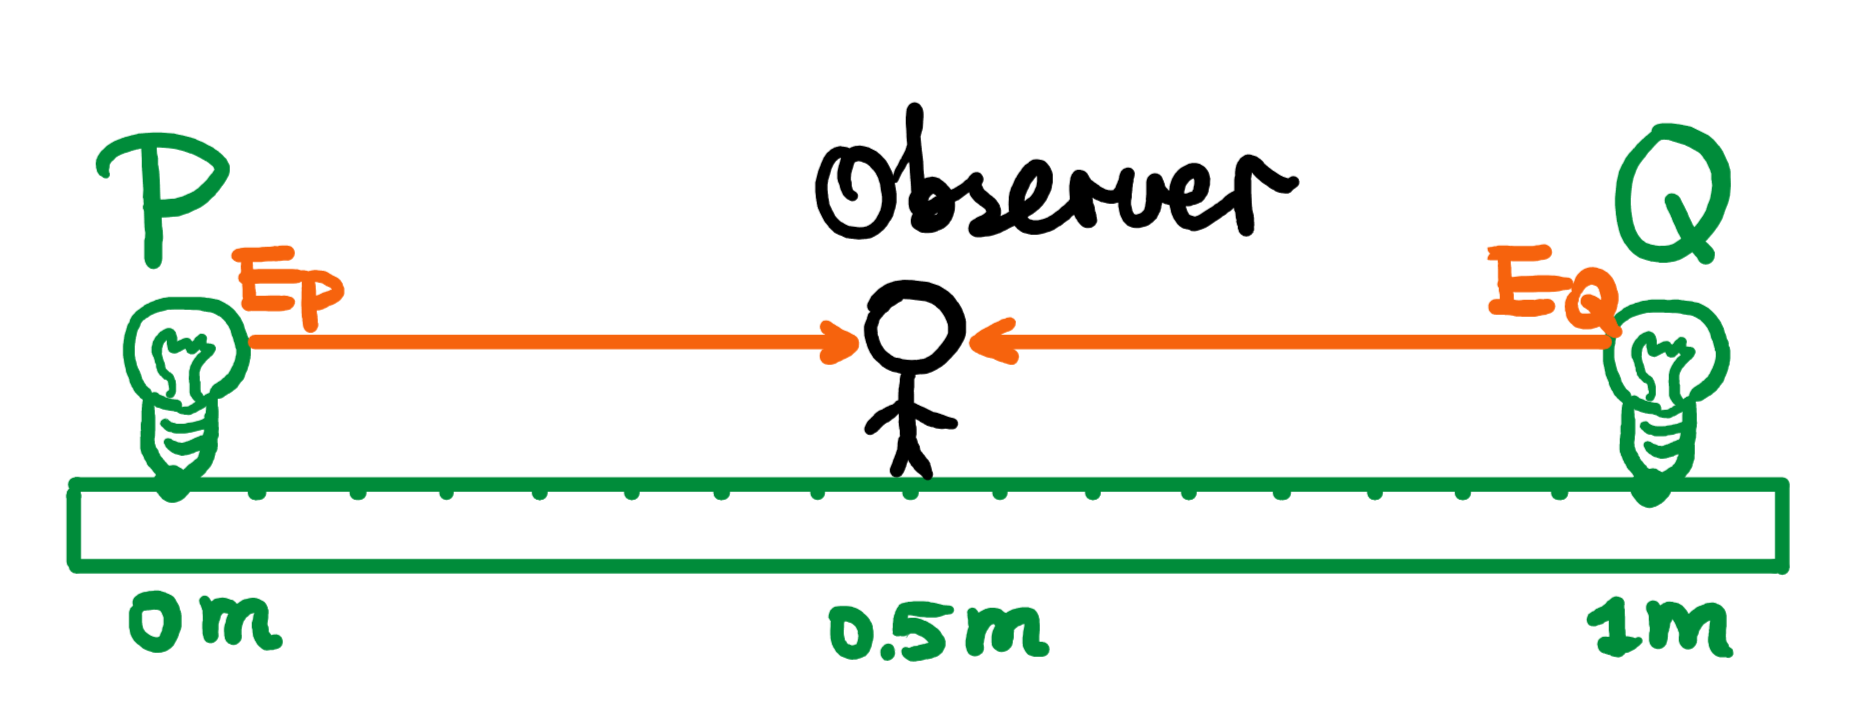
\includegraphics[width=0.4\textwidth]{st_ground}
\mtextbox{关于参考系的时间}{之前我们介绍过参考系的时间——在不同的位置,时间是用光信号同步的,减去光传播所用的时间。这里,同时性的概念意味着$E_P$ 和$E_Q$ 在这个静态框架中发生在相同的坐标时间。}

引入两个事件:事件$E_P$发生在对象$P$上;并且事件 $E_Q$ 发生在对象 $Q$ 上。例如,$E_P$ 和 $E_Q$ 分别是灯泡在 $P$ 和 $Q$ 处的打开时间。回想一下,每个事件都发生在特定的时刻。

现在我们准备好定义 $E_P$ 和 $E_Q$ 是否同时发生,或者一个比另一个早/晚,相对于观察者来说:

如果来自 $E_P$ 和 $E_Q$ 的光信号同时到达观察者,则 $E_P$ 和 $E_Q$ 同时发生。否则,无论哪个更早到达观察者,哪个就更早发生。
}

\mtextbox{我是在浪费你的时间吗?}{
这看来像是在浪费你的时间来解释一些你从幼儿园就已经知道的事情。这没错。然而,在下一步中,我们就会需要高等教育。
\tcblower
爱因斯坦非常谦虚地说:
``我似乎是在以下情况发现了相对论,。正常的成年人从不为时空问题烦恼。在他看来,所有需要考虑的事情在他的童年早期就已经完成了。而我发展得如此缓慢,以至于我长大后才开始怀疑空间和时间。因此,我比普通孩子更深入地探究了这个问题。
}


\textbox {上述场景的时空图}{
	让我们在“时空图”中画出这些事件。时空图将成为研究相对论的有用工具。在时空图上:

	\begin{minipage}
		{0.58\textwidth}
		\titem{
			\item 一个事件是一个点
			\item 光以 $45^\circ$ 角的方向传播
			\item 一个物体(或观察者,除了光)是一条线(称为世界线),$|$斜率$| > 45^\circ$ 
			\item 惯性观察者是一条直线。
            \item 静止的物体是一条平行于 $ct$ 轴的线。
            \item 同时事件平行于 $x$ 轴。
		}
	\end{minipage}
	\hspace{0.02\textwidth}
	\begin{minipage}
		{0.4\textwidth}
		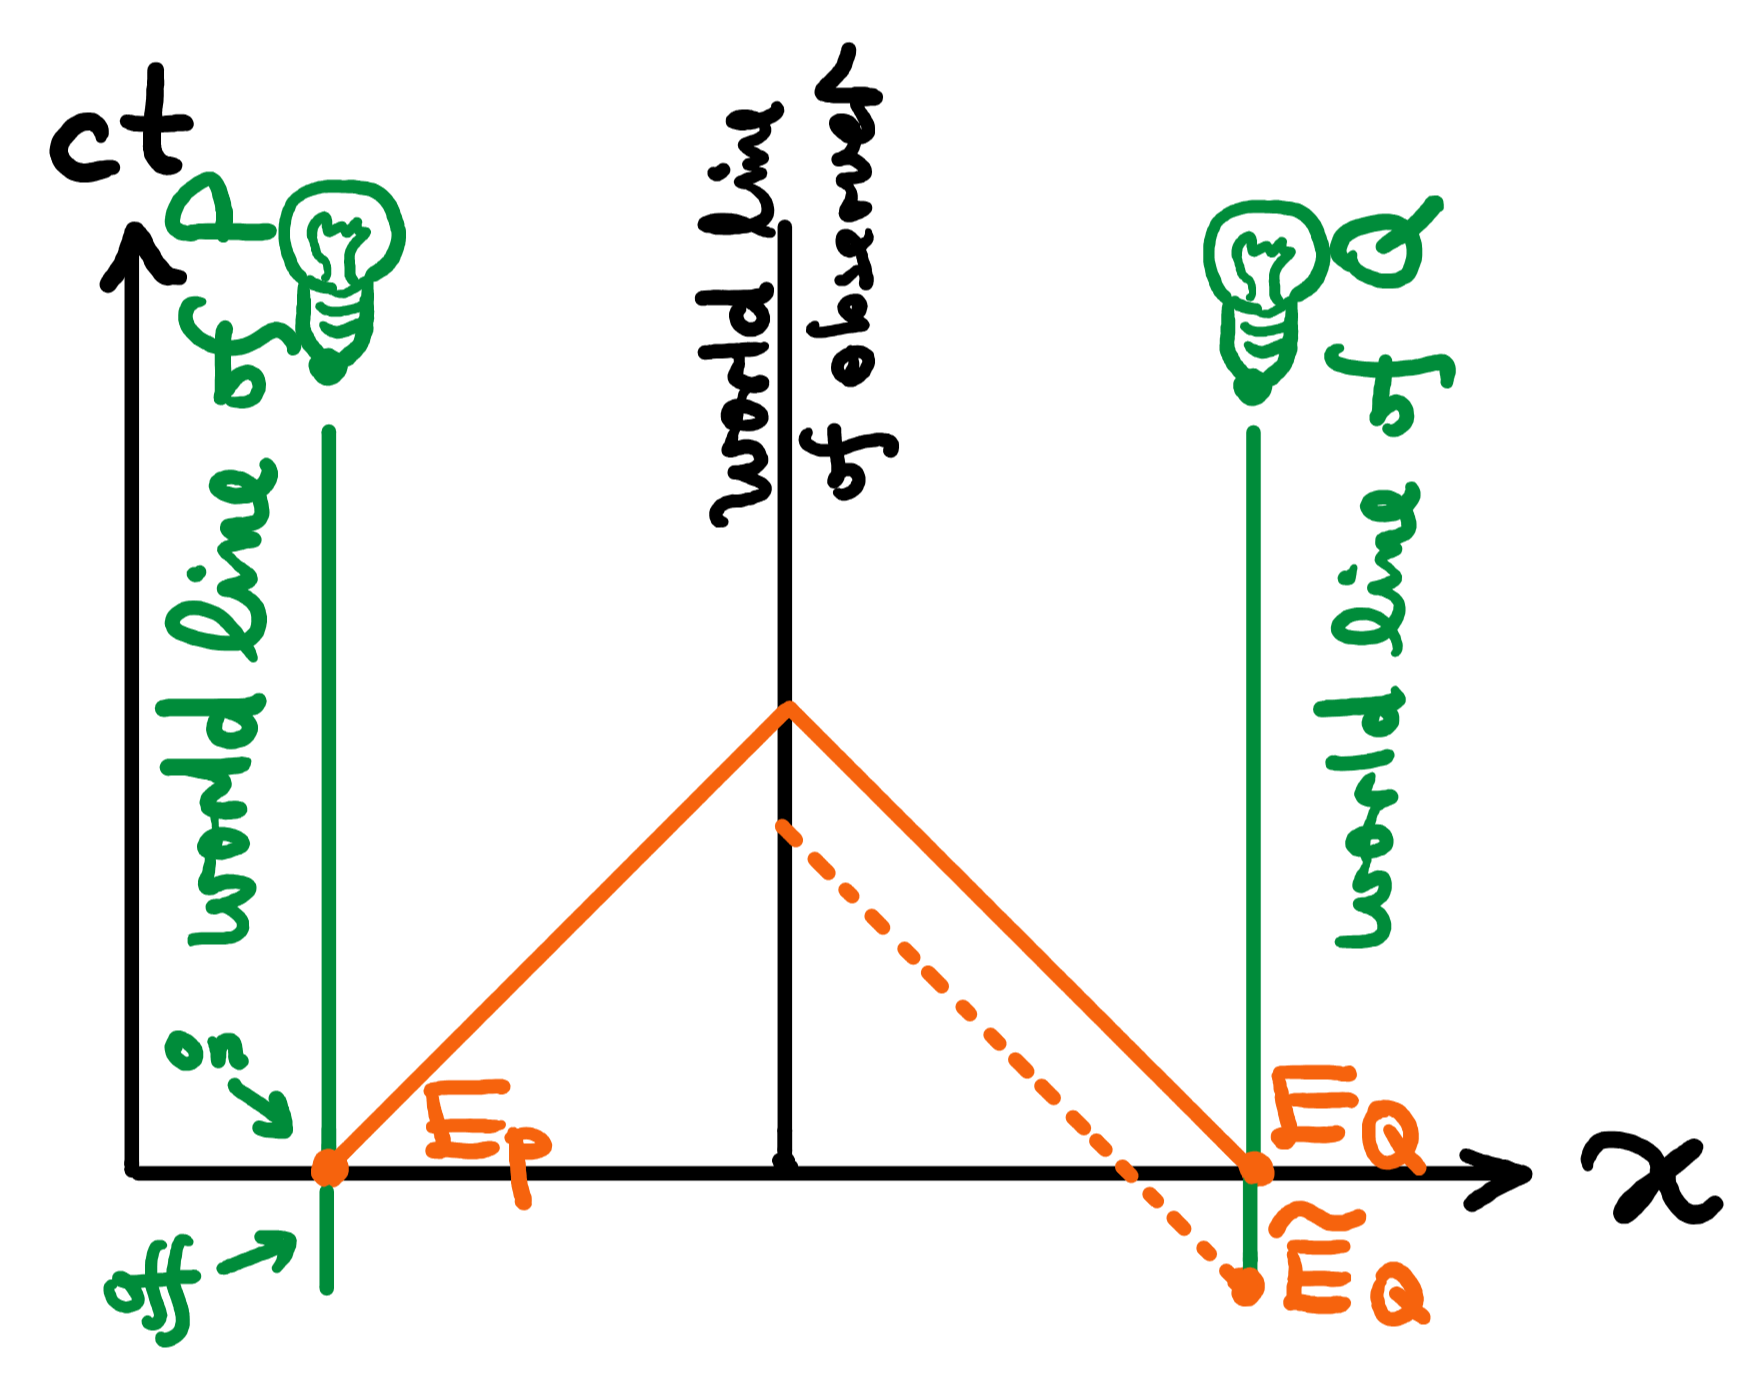
\includegraphics[width=\textwidth]{st_diag_ground}
	\end{minipage}

	如果连接 $E_P$ 和 $E_Q$ 的光线在同一点到达观察者的世界线,则它们相对于观察者同时发生。相反,$\widetilde{E}_Q$ 被认为比观察者的 $E_P$ 更早,因为来自 $\widetilde{E}_Q$ 的光线更早到达观察者。
}

\textbox{同时性是一个相对概念(四步推理)}{\index{同时性是一个相对概念}
	\tenum{
		\item 我们已经用上面的 $P$-observer-$Q$ 系统为静态观察者定义了同时性。
		\item 让我们将这个系统放到汽车中,让移动的观察者是 Alice。 让我们研究一下事件 $E_P$ 和 $E_Q$,它们同时发生在 Alice 身上。 在我们的示例中,这对应于在 Alice 的 $P$ 和 $Q$ 处同时打开的灯泡。 见下图左面板。

		\begin{minipage}
			{0.55\textwidth}
			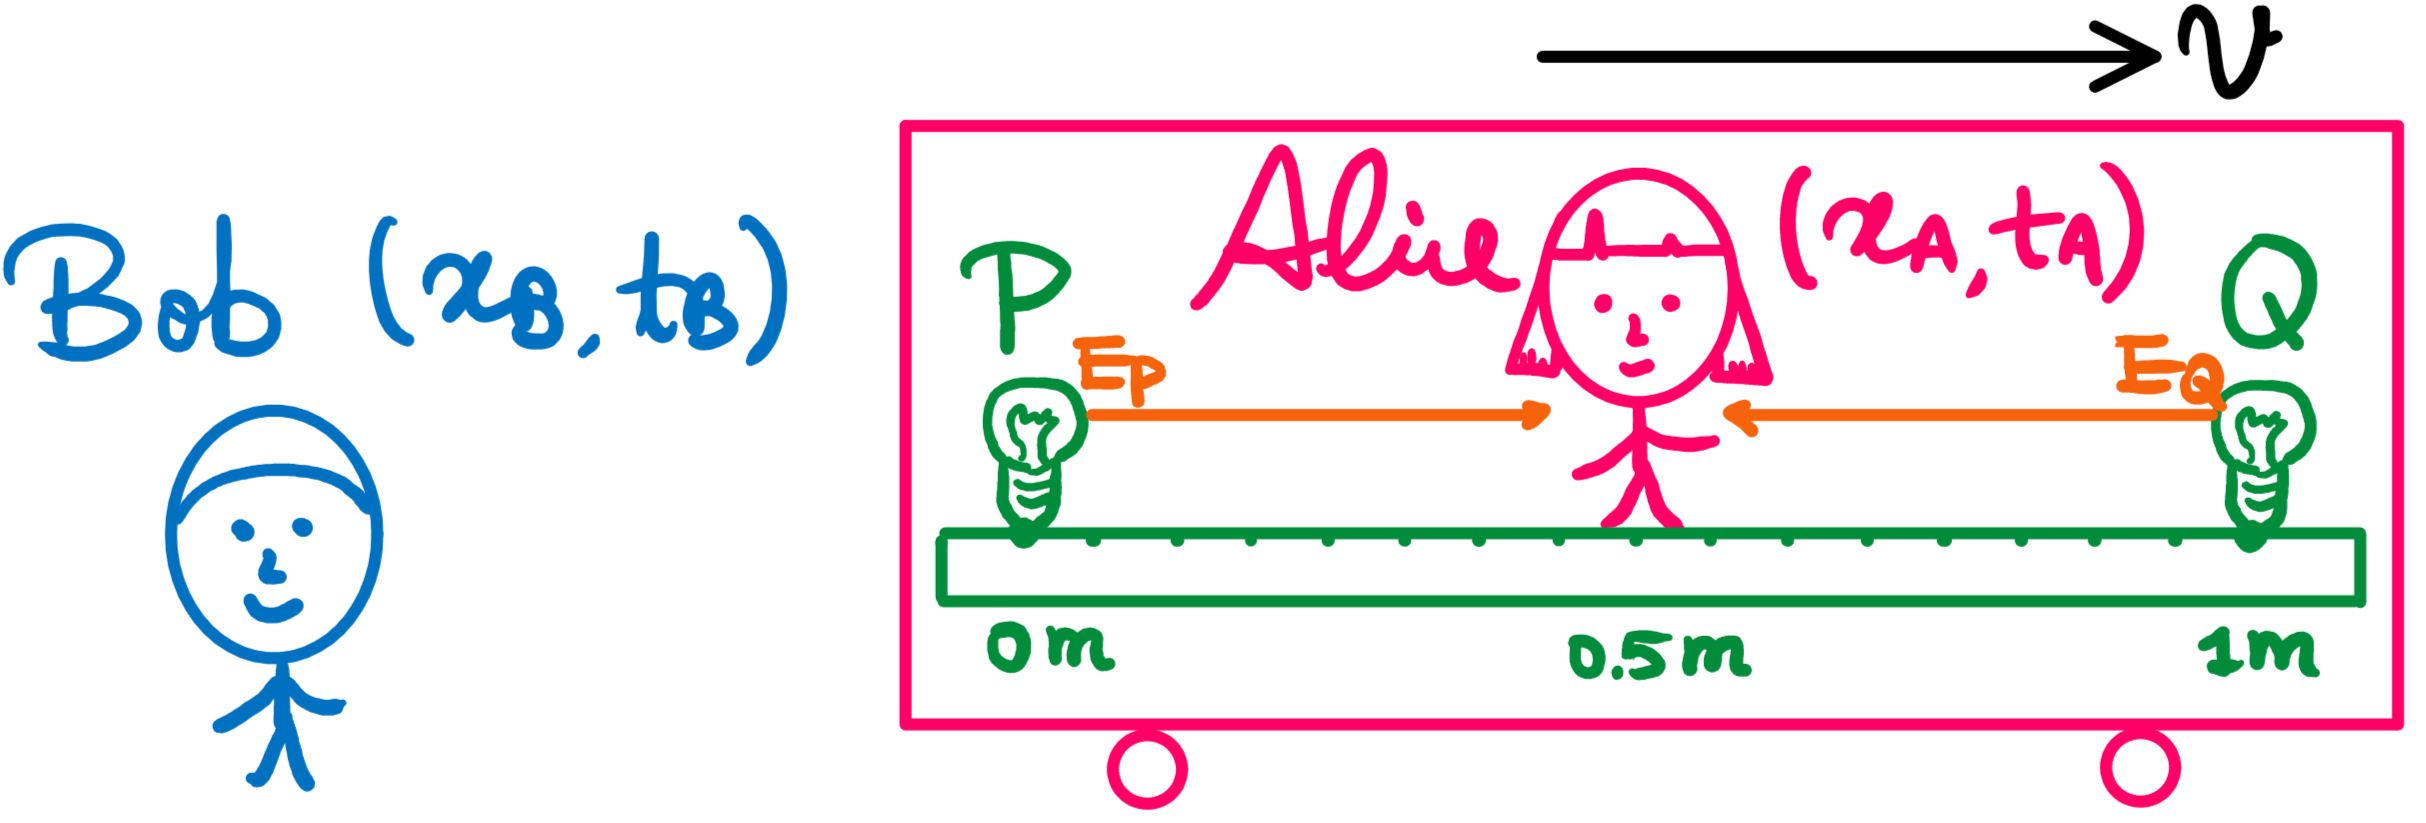
\includegraphics[width=\textwidth]{st_car}
		\end{minipage}\hspace{0.1\textwidth}
		\begin{minipage}
			{0.35\textwidth}
			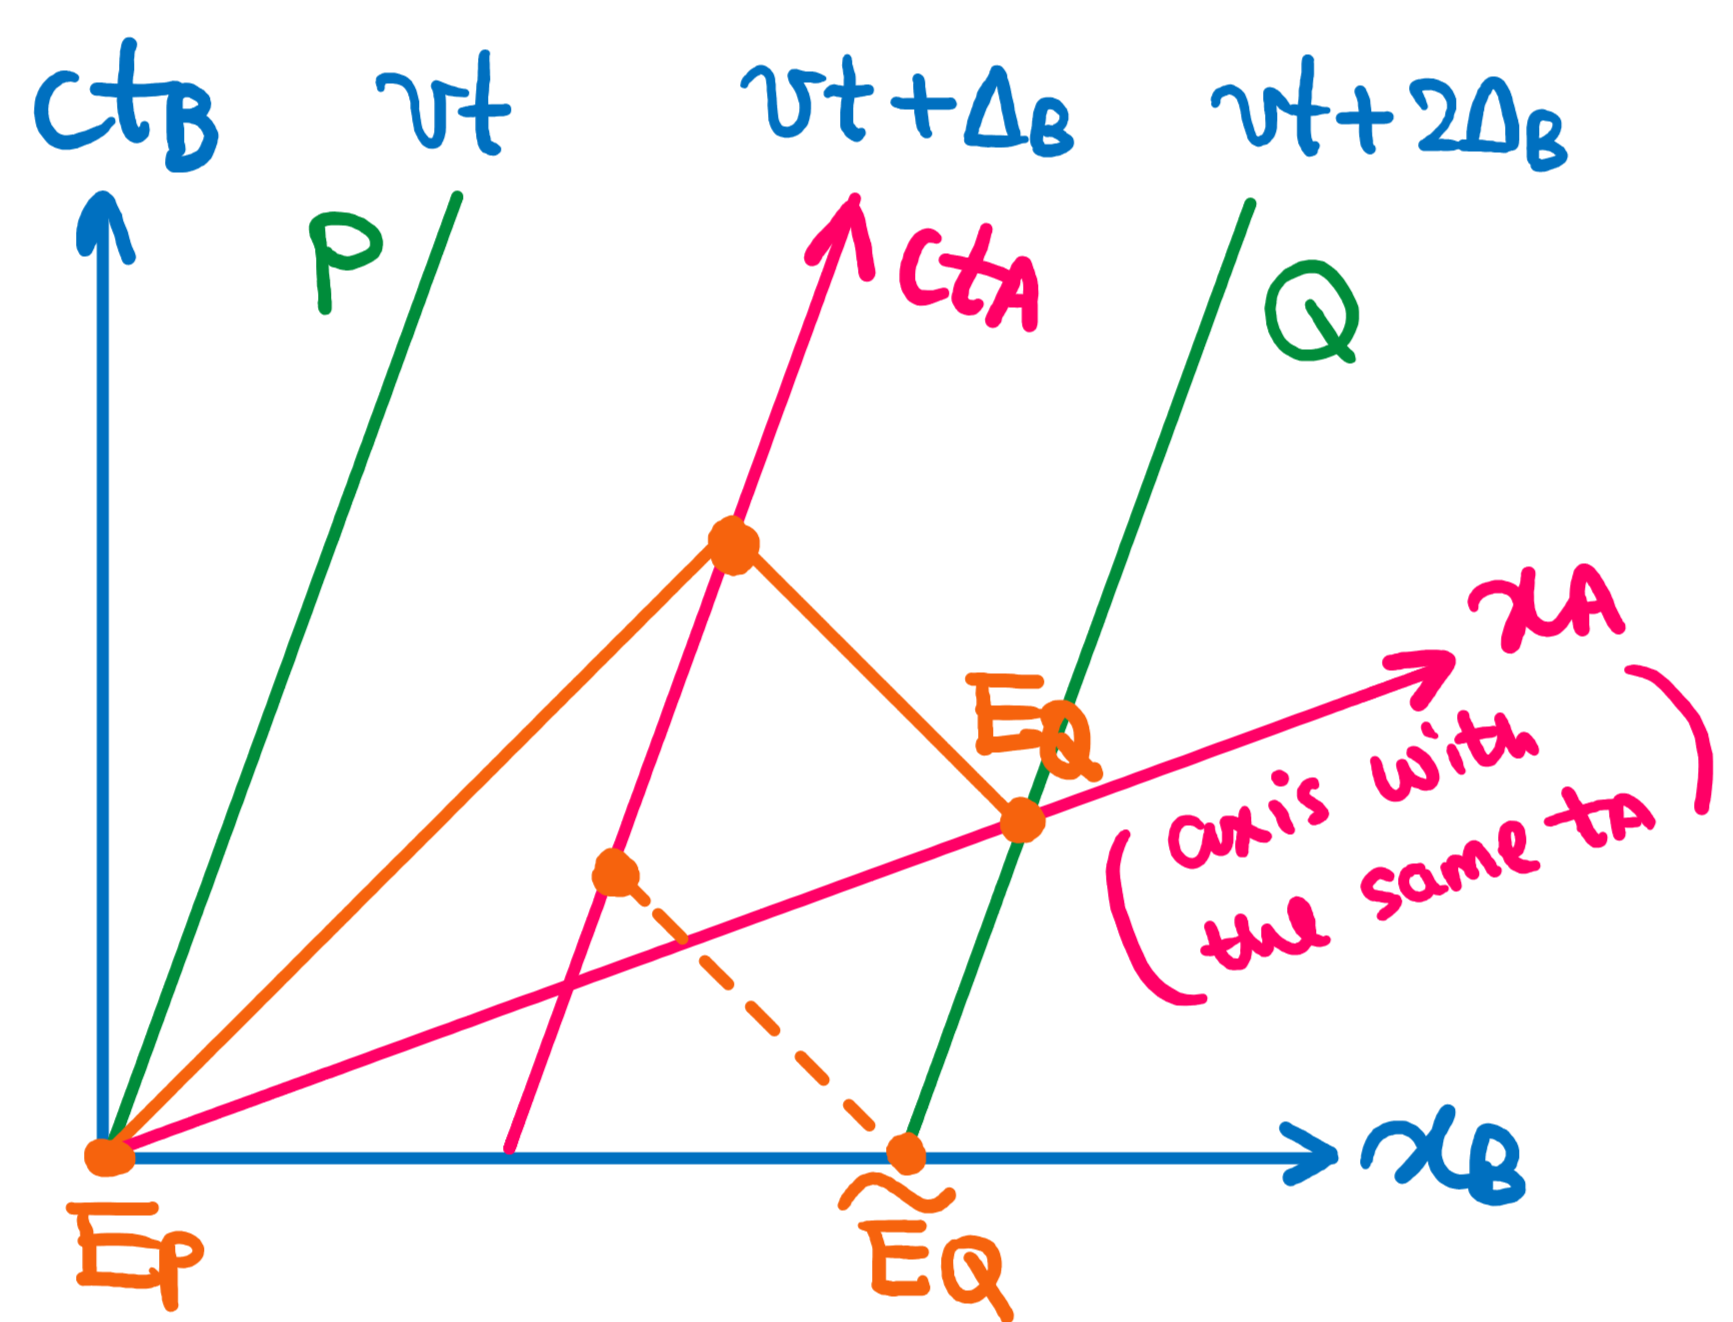
\includegraphics[width=\textwidth]{st_diag_car}
		\end{minipage}

		\mtextbox{Bob的时空图}{
			\mtitem{
				\item 画出Bob的时空轴和世界线 $A$, $P$, $Q$.
				\item 画出两束光线同时到达Alice
				\item 将这两束光的历史画成 $45^\circ$ 线
				\item 光与$P$、$Q$的交点是事件$E_P$、$E_Q$。
				\item 比较在Bob参考系中 $E_P$ 和 $E_Q$ 的时间
				\item 在 Bob 的参考系中画出 Alice 参考系的时空轴。
			}
		}
		\item 相对于Bob,$E_P$ 和 $E_Q$ 是否同时发生? 换句话说,$E_P$ 和 $E_Q$ 在 Bob 的坐标系中是否具有相同的时间坐标? 利用 Bob 框架中的时空图(上图右图),我们立即发现 $E_P$ 比 Bob 早于 $E_Q$。 相反,一个事件 $\widetilde{E}_Q$ 被认为与鲍勃的 $E_P$ 同时发生,被认为早于爱丽丝的 $E_P$。
		
		\item 同时性的相对性不仅适用于 $P$-observer-$Q$ 系统,而且适用于所有一致的同时性定义 ($\mathbb{R}$)。
	}
}
现在你应该可以解决“谁先写这封信”的难题了。

\textbox{回顾: 相等的时间片段}{
	\begin{minipage}
		{0.55\textwidth}
		把上面的分析浓缩成一张图:当爱丽丝向鲍勃移动时,爱丽丝在鲍勃坐标系中绘制的坐标系如右图所示。 它类似于旋转,但空间和时间轴都奇怪地向内折叠。 稍后我们将更详细地讨论这种变换(洛伦兹变换)。 你应该特别注意这张图上相对于爱丽丝的相等时间线——与相对于鲍勃的不同。
	\end{minipage}
	\hspace{0.1\textwidth}
	\begin{minipage}
		{0.35\textwidth}
		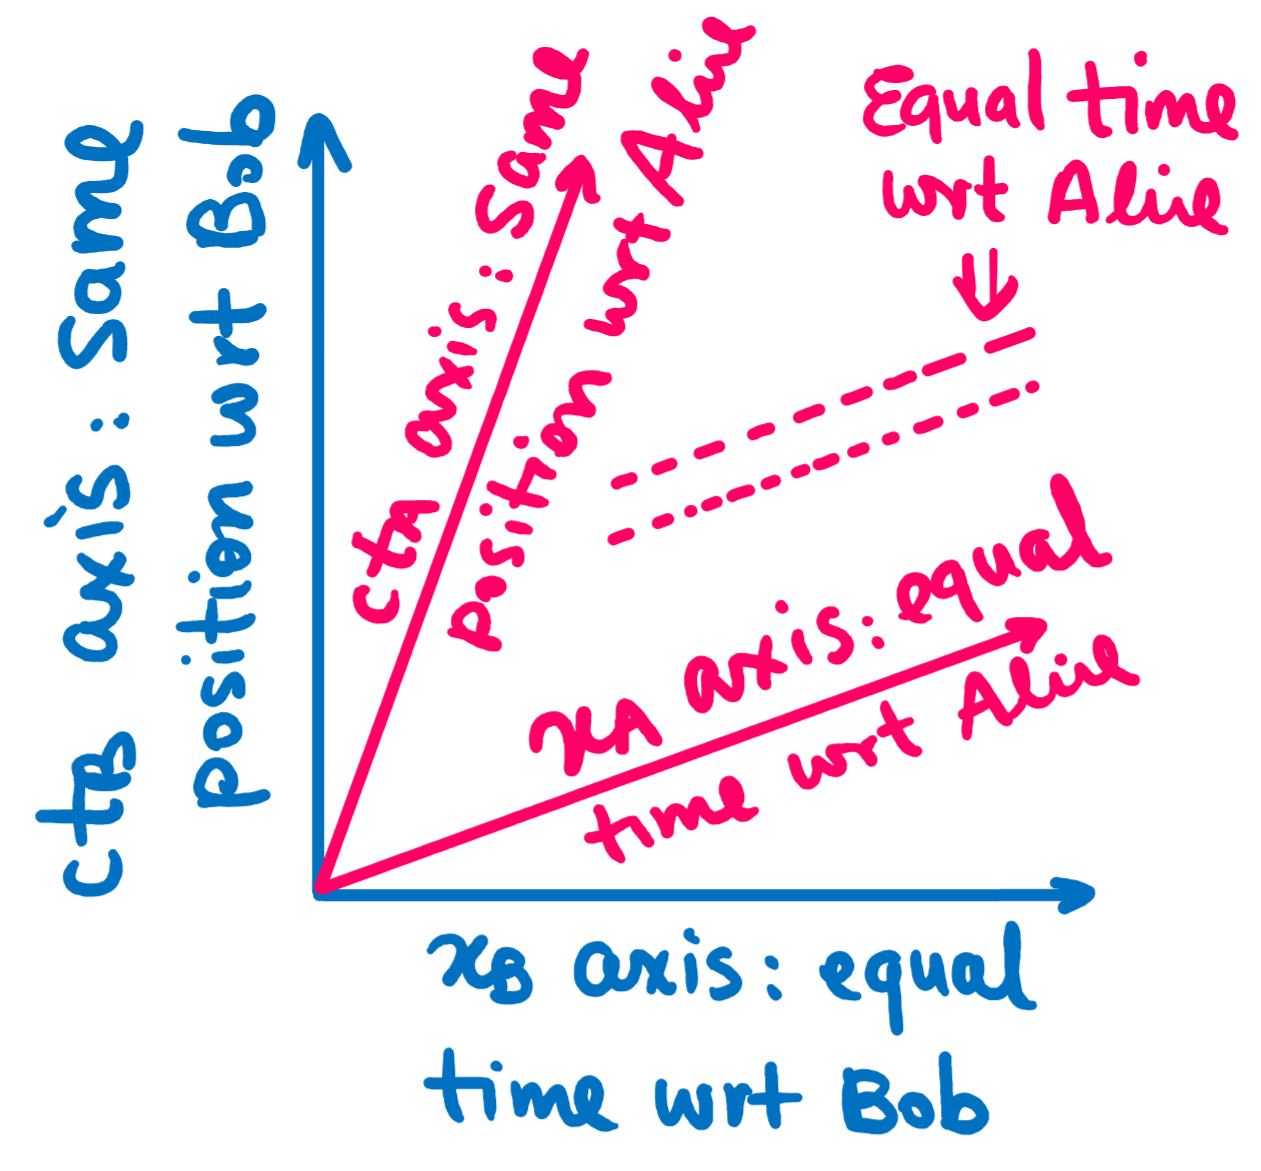
\includegraphics[width=\textwidth]{equal_time_simplified}
	\end{minipage}
}

\mtextbox{狭义相对论可以描述加速度吗?}{有一个常见的误解是“狭义相对论不能描述加速观察者”. 这是 \emph{错误的}。 狭义相对论的定律(时间膨胀、长度收缩等)用惯性坐标系表示(只是因为惯性坐标系中的定律在数学上更简单)。  因此,我们需要 \emph{使用惯性参考系} 将这些定律应用于我们的问题。 然而,我们可以\emph{在这个惯性参考系中计算}加速观察者看到的东西(例如,光线如何到达她的眼睛)。 这样,加速观察者的经验被描述为\emph{在辅助惯性系的帮助下}}
\textbox{再谈双生子佯谬}{\index{再谈双生子佯谬}
	\begin{minipage}
		{0.6\textwidth}
		在我们的双生子佯谬中,爱丽丝在转弯时并不是惯性观察者。 因此她不能用惯性观察者的狭义相对论来\emph{直接}解释她的经历。 然而,鲍勃可以帮助她弄清楚在她调头时会发生什么:

		在转弯前后,Alice 处于两个 \emph{不同的} 惯性坐标系中。 当爱丽丝从转身前的参考系切换到转身后的参考系时,鲍勃的年龄“突变”了。 因此,在 Alice 的框架中,Bob 的年龄突然发生了变化。

		如前所述,为了描述 Alice 看到的东西(考虑到她眼睛的距离),需要加上光传播时间。 
		
	\end{minipage}
	\hspace{0.01\textwidth}
	\begin{minipage}
		{0.3\textwidth}
		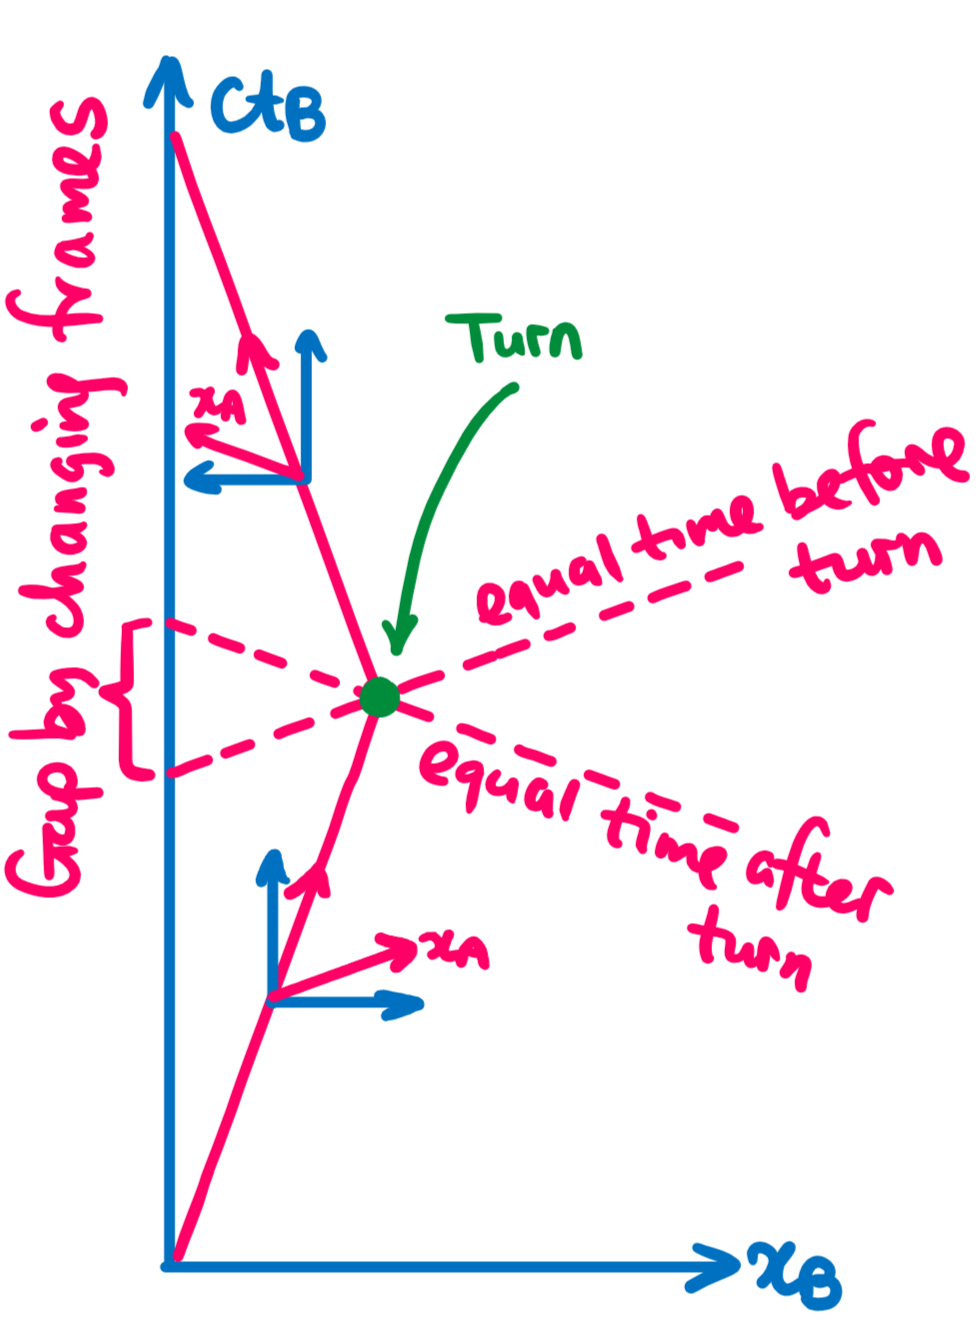
\includegraphics[width=\textwidth]{same_time_twin}
	\end{minipage}
}

\subsection{因果关系和分离类型}

现在我们明白了:同时性的概念是相对于观察者而言的。例如,爱丽丝和鲍勃可能会以不同的方式考虑谁先写了这封信。换句话说,一些事件(这里有两个事件:Alice 写她的信和Bob 写他的信)的时间顺序是可逆的。

那么一个自然的问题是:事件之间的所有时间顺序都是可逆的吗?

\textbox{与因果相关的时间顺序}{\index{因果关系}
	考虑一个例子:闪电击中一棵树,然后树就死了。这里有两个事件:
	\marginnote{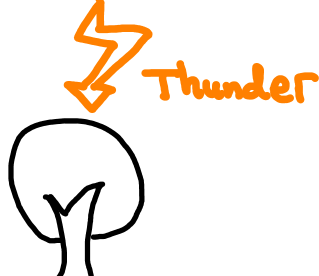
\includegraphics[width=0.15\textwidth]{thunder}}
	\tenum{
		\item 事件E(击中): 闪电击中了树
		\item 事件E(树死了): 树死了 \emph{事件}, \emph{因为} 事件E(击中)
	}
	一个移动的观察者有可能观察到树死了比闪电击中树更早发生吗?

	\mtextbox{相关性}{因果关系是相关性的一个特例。 如果事件 E1 和 E2 具有并不显然的相关性,也许
	\mtitem{
		\item E1 导致了E2
		\item E2 导致了 E1
		\item  E1 和 E2 发生的原因都是其他事情
	}}
	\tcblower
	因果关系是物理学的核心。 物理学是关于预测状态如何随时间演变的(从初始状态开始)。 换句话说,因果关系是物理学中如何解释问题——“为什么产生了某个效果? 因为某种原因。''
}

由于因果关系如此重要,我们希望它在狭义相对论中得以保留。 令人高兴的是,狭义相对论确实与因果关系 \emph{具有一致性}。 话虽如此,因果关系是添加到狭义相对论的独立假设。 换句话说,狭义相对论本身并不能\emph{推导出}因果关系。 现在让我们看看因果关系和相对论是如何协同工作的。

\mtextbox{超光速的闪电也是不存在的}{
遵循因果顺序,不仅布莱特女士不应该超光速旅行,闪电(或任何导致树木死亡的信息)也不可以是超光速的。 否则,即使是对于运动的比光速慢的布莱特女士,也违反了因果关系。}

\textbox{没有超光速运动的狭义相对论与因果关系具有一致性}{\index{因果关系和相对论}
	\begin{minipage}
		{0.5\textwidth}
		不超光速的Ms. Bright和超光速的Ms.~Bright的时空图。 对于任何超光速观察者来说,这棵树的世界线的斜率大于 $45^\circ$。 那么,只要 Ms.~Bright 的移动速度不超过光速,她就不能颠倒 E(树被击中) 和 E(树死了) 的顺序。
	\end{minipage}
	\hspace{0.05\textwidth}
	\begin{minipage}
		{0.4\textwidth}
		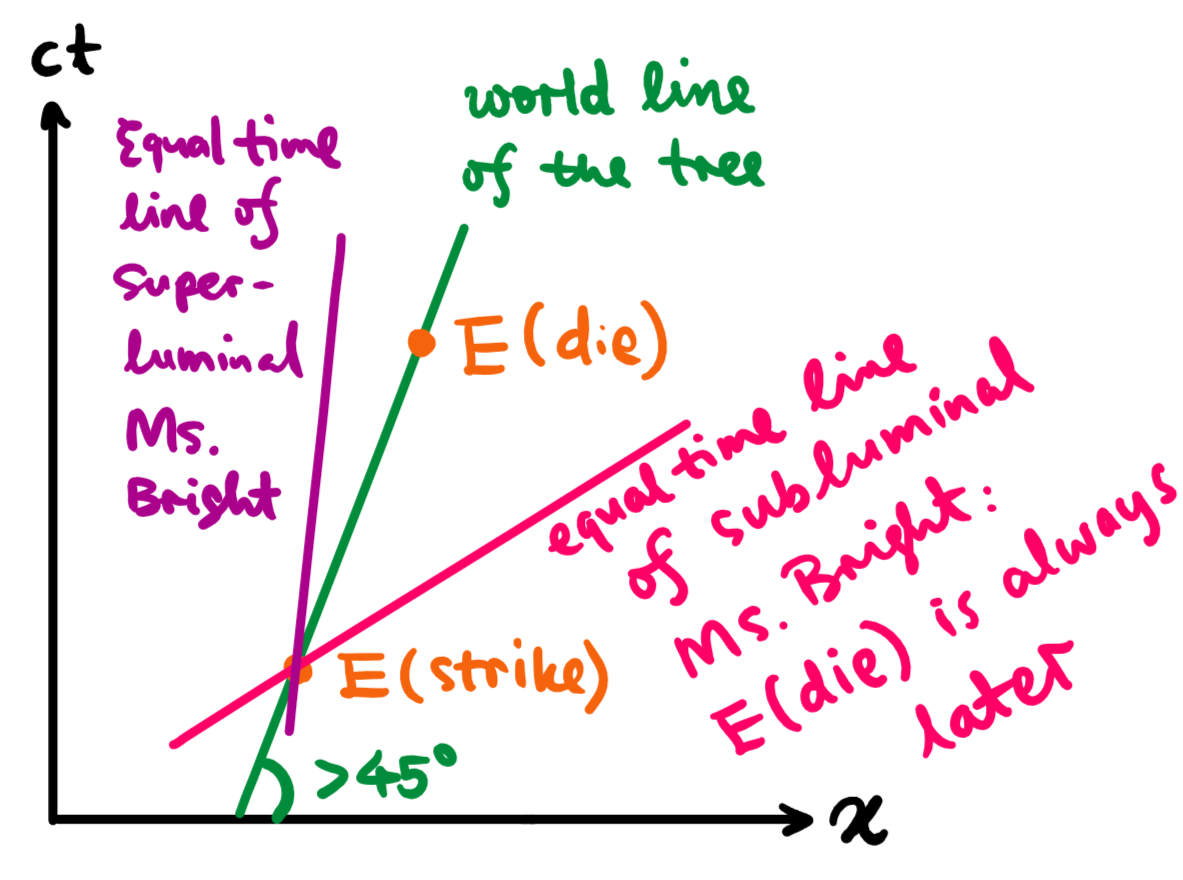
\includegraphics[width=\textwidth]{sr_consistent_causality}
	\end{minipage}

	\mtextbox{Buller's 的诗 (1923)}{
	There was a young lady named Bright;\newline
	Whose speed was far faster than light;\newline
	She set out one day;
	In a relative way;\newline
	And returned on the previous night.	\mnewline
	We hope this to be forbidden. Otherwise, what if Ms.~Bright returned to the previous night, and locked herself in the room, how can her superluminal trip happen at all? \mnewline
	So far, the most convincing explanation is that, superluminal trip should be forbidden. Having that said, the possibility of a time machine is an open question for modern physics.
	}
	\tcblower

	因此,如果禁止超光速的运动,则保留因果顺序。 在本课程中,我们将假设在狭义相对论中确实不允许超光速运动。 这与所有已知的实验一致。

	更一般地来说,没有任何信息可以比光速传播得更快。 因为信息必须通过物质来传递。 并且从理论的一致性来看,信息可以带来事件之间的因果联系。 因此,如果信息可以比光更快地发送,那么超光速运动的问题就会出现。

	此时你可能有一个很好的问题:如果我们推动 Ms.~Bright 让她从超光速加速到超光速会怎样? 事实上这是不可能的。 我们稍后会回到这一点。

	在广义相对论中,你可能听说事物可以超光速,例如宇宙膨胀。 这是对还是错。 首先必须精确定义速度。 我们将在本课程结束时的宇宙学部分回到这一点。
}


\textbox{时空的因果结构:过去和未来的光锥\index{光锥}}{
	分离事件来看,给定一个时空点(比如现在的你),根据与事件的因果联系,将时空划分为三个不同的区域。
	\marginnote{\cg{0.3}{lightcones}}

	\titem{
		\item 过去的光锥: 这个区域包含了你到现在为止的所有原因。 除了这个区域,你还没有看到任何东西。
        \item 未来的光锥: 该区域包含您从现在开始的所有效果。 您无法再更改此区域之外的任何内容。
        \item 在过去和未来的光锥之外:现在的你和那里的任何一点之间都没有因果关系。
	    }
}
\textbox{相对论中没有完美的刚体}{\index{刚体(不存在)}
让我们考虑一个思想实验:爱丽丝和鲍勃相距 5 光年。 而且他们手里拿着一根5光年长的杆子,这是一个完美的刚体。 那么爱丽丝和鲍勃可以通过推杆以比光速更快的速度发送信息吗?

	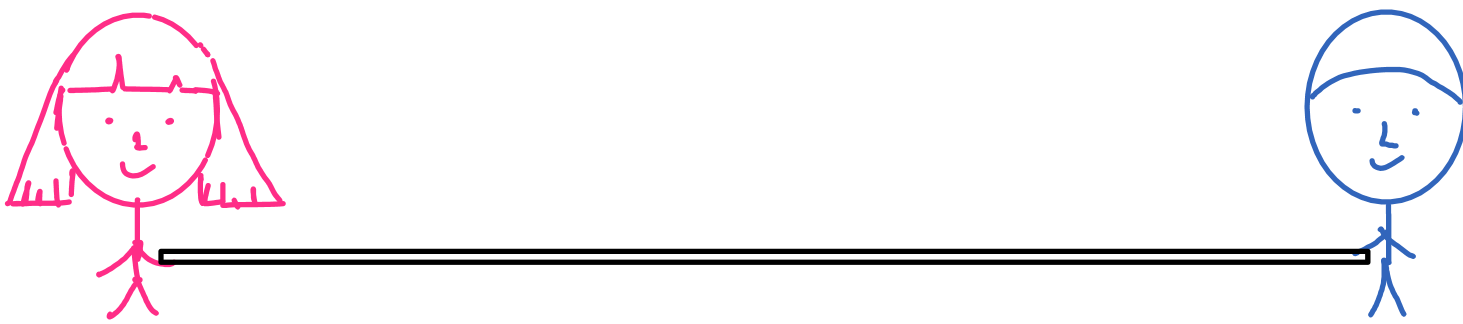
\includegraphics[width=0.8\textwidth]{ABrod}

	\tcblower

	答案是一个简单的直接否定。 因为没有信息可以比光快,所以狭义相对论中不存在完美刚体。

如果这个答案太粗鲁,我们也可以动态地看到发生了什么。 杆子(通常)由原子制成,在原子之间传播的力至少需要光速才能对推动作出反应。
}

光速极限将两个事件之间的区间分为 3 类。

\textbox{类空间隔、类时间隔和类光间隔}{\index{类空间}\index{类时间}\index{类光(零)}
	
	\marginnote{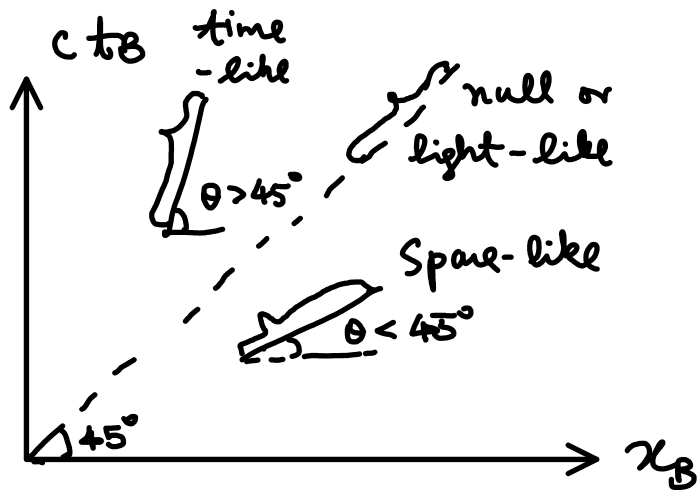
\includegraphics[width=0.35\textwidth]{space_time_null_like}}
	事件之间有三种间隔。
	\titem{
		\item 类空间:斜率 $<45^\circ$。 存在两个类似空间的分离事件同时发生的观察者。 因此,这些事件与这个观察者是纯空间分离的。 事件的时间顺序可以因不同的观察者改变。
        \item 类时间:斜率 $>45^\circ$。 存在两个类似时间的事件发生在同一位置的观察者。 因此,事件仅在这个观察者的时间上被分开。 事件的时间顺序是绝对的,必须为所有观察者达成一致。
        \item 类光(或称为零):分隔类空间和类时间间隔的边界,斜率为 $45^\circ$。 光以类似光的线条传播。
	}
}

\section{例: 梯子悖论}\label{sec:ladder}

让我们应用我们学到的东西来把自己搞糊涂(或希望不会)。

\textbox{梯子和车库}{\index{梯子悖论: open garage}
	考虑一个 15m 长的梯子(两端标记为 P 和 Q)。 Alice 拿着它,将它移向车库,速度为 0.87c,即 $\gamma=2$。 车库长10m,前门和后门分别标有F和B。 鲍勃坐在车库里,一动不动。

	\cg{0.7}{ladder}

	\marginnote{\hfill 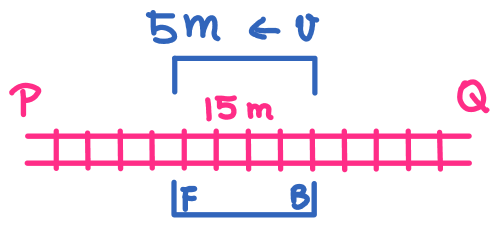
\includegraphics[width=0.25\textwidth]{ladderA}\hspace{0.02\textwidth}}
	
	爱丽丝发现了什么? Alice 发现车库移动了,因此车库的长度为 $10\mathrm{m}/2=5\mathrm{m}$。 因此梯子不适合车库。

	鲍勃发现了什么?Bob发现梯子移动了,因此梯子的长度为 $15\mathrm{m}/2=7.5\mathrm{m}$。 因此梯子适合车库。

	\marginnote{\hfill 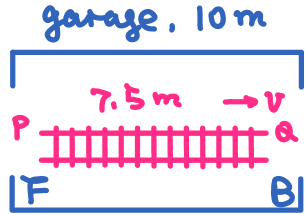
\includegraphics[width=0.2\textwidth]{ladderB}\hspace{0.02\textwidth}}

	谁是正确的?

	\tcblower

	\twocol{0.5}{0.01}{0.75}{
		他们都是正确的。
		
		Note that ``ladder fit in garage'' is not an event which localized at a spacetime point. Especially, there are two important events:

		\tenum{
			\item P进入前门F
			\item Q从后门B出去
		}

		如果 \enumlabel{1} 早于 \enumlabel{2},则梯子适合车库。 如果 \enumlabel{2} 早于 \enumlabel{1},则梯子不适合车库。

		如果 \enumlabel{1} 早于 \enumlabel{2},则梯子适合车库。 如果 \enumlabel{2} 早于 \enumlabel{1},则梯子不适合车库。
	}{
		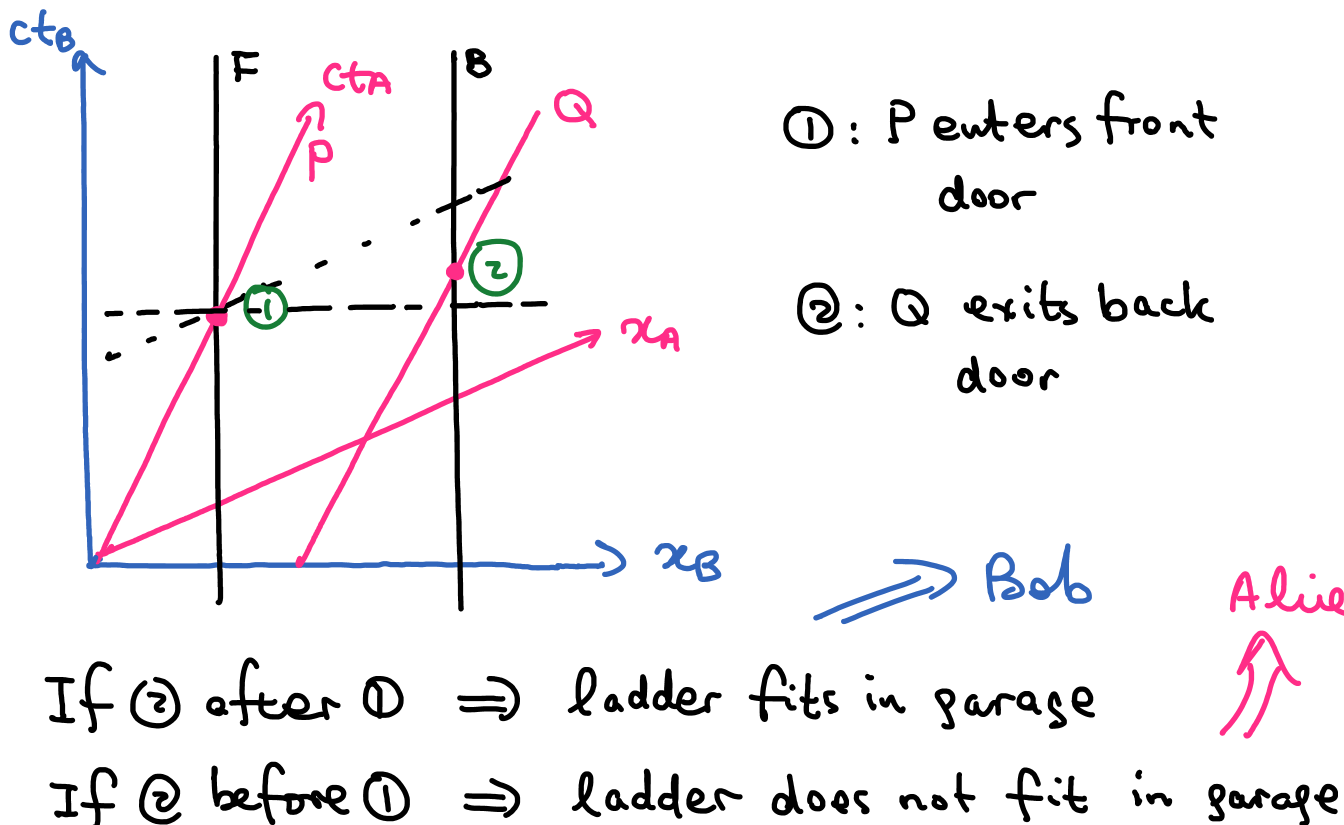
\includegraphics[width=\textwidth]{garage_st}
	}
}

\textbox{梯子和带门的车库}{\index{梯子悖论:封闭车库}
\marginnote{这里我们假设爱丽丝仍然在一个内部框架中,无论梯子的任何部分可能停止或不停止。 }

让我们添加一个本地事件来加强发生的事情。 让车库的后门永远关闭。 鲍勃发现车库里的梯子移动了,就关上了前门。

	\cg{0.7}{garage_door}

	现在即使是爱丽丝也不得不同意梯子完全在车库里,因为门是关着的。 所以“悖论”变得更加尖锐:爱丽丝认为梯子比车库长; 但它现在完全在车库里!

    解决方案:请记住,在相对论中,没有完美的刚体。

    假设门相对坚固且不断裂,那么梯子肯定会分成几部分。 Wrt Alice:当 Q 停止移动时,必须将“停止”信息传递给 P,并且至少需要 $15\mathrm{m}/c$ 的时间。 在此期间,前门移动了大约 13 美元。 因此,此时 $P$ 完全在 $F$ 之内。 当然,它非常适合 5 美元的车库。

    反之,如果梯子比较坚固,不破,那么后门破了,和没有后门没有区别。
}

\textbox{用陷阱代替车库}{\index{梯子悖论:陷阱}
	让我们进一步用陷阱的边界替换二个门。
	
	\cg{0.7}{trap}

	Bob' 认为当梯子完全落入陷阱时,带梯子的 Alice 开始掉入陷阱。 因此爱丽丝坠入了。然而,爱丽丝认为在Q点逃逸之前自己还没有坠入。 谁是对的?
	\tcblower
	这真的取决于爱丽丝如何拿着梯子。 如果爱丽丝拿着梯子完全平行于地面并在地面上滑动,那么爱丽丝就会掉进去。因为没有完美的身体。 当$Q$落入陷阱时,$Q$不可避免地会往下掉。 但是,如果 Alice 把梯子稍微往上一点,这样 Q 从一开始就不需要地面支撑,那么 Alice 可以逃跑。
}

\textbox{用电路代替车库}{\index{梯形悖论:电路}
	让我们停止破坏事物,走向电子化。 考虑下面的情况。

	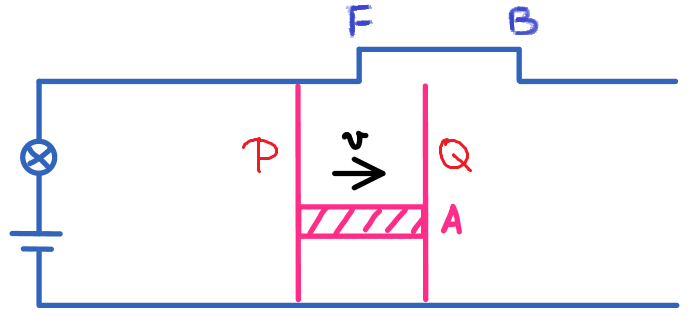
\includegraphics[width=0.6\textwidth]{light_paradox}

	爱丽丝拿着两条移动的导线(它们彼此隔离)。 两者都可以闭合电路。 鲍勃,有一段时间,爱丽丝的两条电线都没有关闭电路,所以灯泡会暂时关闭。 相对于Alice,至少有一根电线一直接触电路。 那么灯泡要关掉吗?
	
	\tcblower
	解决问题的关键是,电需要时间来传导。 电的速度与$c$相当,但仍低于$c$。 因此,对于 Alice,为了使灯泡在没有关闭时间间隙的情况下保持打开状态,电流必须在 Q 超过 F 之前达到 F。所以对于 Alice,也有一个关闭时间。
}


\section{洛伦兹变换} \label{sec:lorentz}

\textbox{Alice 和 Bob 需要遵循一个规则来进行坐标变换}{

	\twocol{0.55}{0.1}{0.3}{
		发生了 $P$ 事件。 移动的 Alice 和站立的 Bob 都同意事件的存在。 但是,同一事件在 Alice 和 Bob 的参考系中具有不同的坐标。

        给定 P:$(t_B, x_B)$ 在 Bob 框架中的坐标,如何得到 Alice 框架中同一事件的坐标 $(t_A, x_A)$?
	}{
		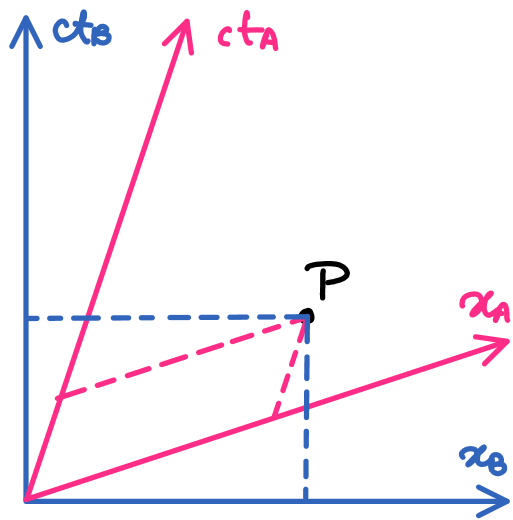
\includegraphics[width=\textwidth]{st_trans}
	}

	回想一下,惯性系之间的转换称为推动变换。 因此这个问题也可以这样问:坐标在推动的时候是如何变换的?

	\tcblower

	在解决这个问题之前,让我们画出推动和旋转之间的相似性。

	\twocol{0.5}{0.05}{0.45}{
		旋转的情况:Alice 和 Bob 并没有相互移动,而是面向不同的方向。 给定 Bob 的对象 $(x_B, y_B)$ 的坐标,如何获得 Alice 对同一对象 $(x_A, y_A)$ 的坐标? 根据欧几里得几何关系,我们得到: \index{旋转}
		
		\begin{equation}
			\label{eq:ss-rotation}
			\left\{
			\begin{aligned}
				x_A & = x_B \cos\theta + y_B \sin\theta \\
				y_A & = -x_B \sin\theta + y_B \cos\theta
			\end{aligned}
			\right.
		  \end{equation}
	}{
		  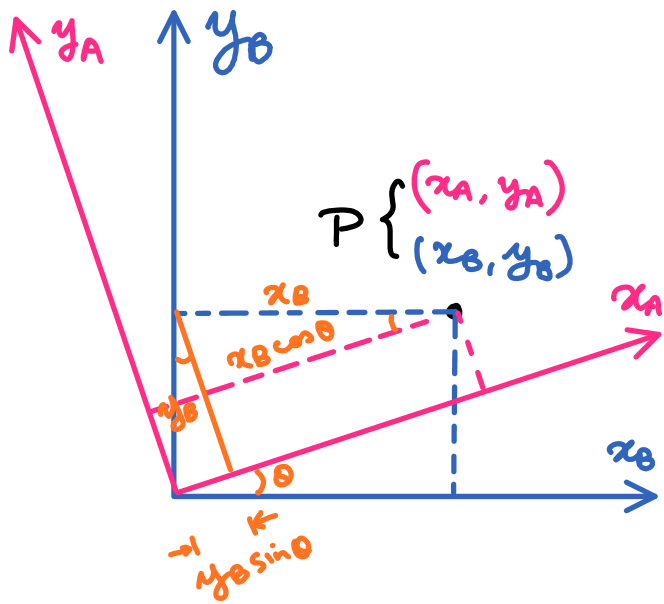
\includegraphics[width=\textwidth]{ss_trans}
	}
	希望你通过这个类比对这个问题有更好的了解。 此外,在下一节中,我们将发现这些时空变换和时空变换之间惊人的相似性。
}

\mtextbox{大体方向的速度}{
	请注意,参考系之间的相对速度 $v$ 仅沿 $x$ 方向(对 Bob 为正)。 如果您正在处理大方向 $\mathbf{v} = (v_x, v_y, v_z)$ 的速度,您可以在应用变换之前先进行旋转以将其旋转到 $x$ 方向。
}
\textbox{Space transformation of a boost}{\index{Lorentz transformation: space}
	\twocol{0.55}{0.1}{0.35}{
		给定 Bob 的坐标 $(t_B, x_B)$,现在我们要求解 $x_A$。 怎么做? 一个等效的问题是,如何在物理上描述 $x_A$? 注意 $x_A$ 是 Alice 的空间坐标。 因此,如果 Alice 携带一个长度为 $x_A$ 的尺子(静态的 Alice),Alice 持有一端,那么另一端的坐标为 $x_A$。
	}{
		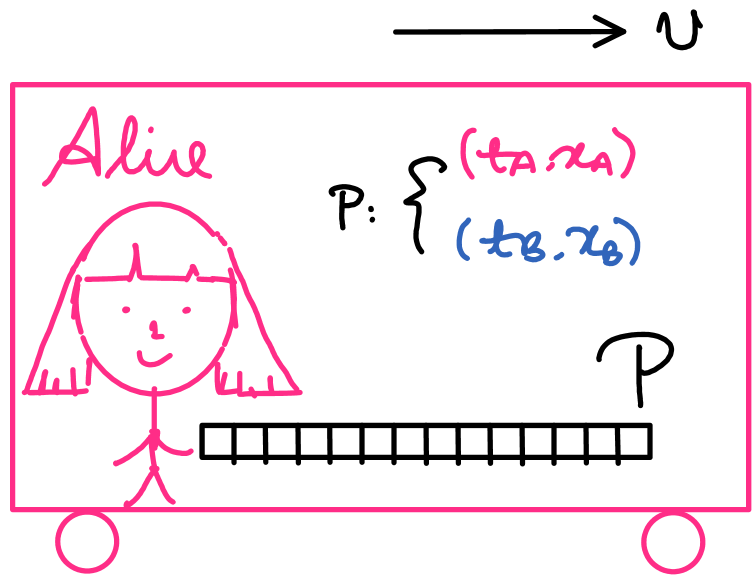
\includegraphics[width=\textwidth]{rr1_reduced}
	}

	\twocol{0.6}{0.05}{0.35}{
		为简单起见,我们为 Bob 和 Alice 选择相同的坐标原点。 给定 Bob 的 P 坐标:$(t_B, x_B)$,我们如何找到关系 $x_A(t_B, x_B)$?

        对于 Bob,移动标尺的长度为 $x_A/\gamma$。 因此在 Bob 的时间 $t_B=0$,点 P 有 $x_B=x_A / \gamma$。 然而,在 $t_B\neq 0$,端点 P 也移动了距离 $v t_B$。 因此对于一般的$t_B$,$x_B = x_A/\gamma + v t_B$。 换句话说,我们得到 $x_A(t_B, x_B)$(即 $x_A$ 作为 $t_B$ 和 $x_B$ 的函数)为
		\begin{align}
			\label{eq:st_space}
			x_A = \gamma \left ( x_B - v t_B \right )~.
		\end{align}
	}{
		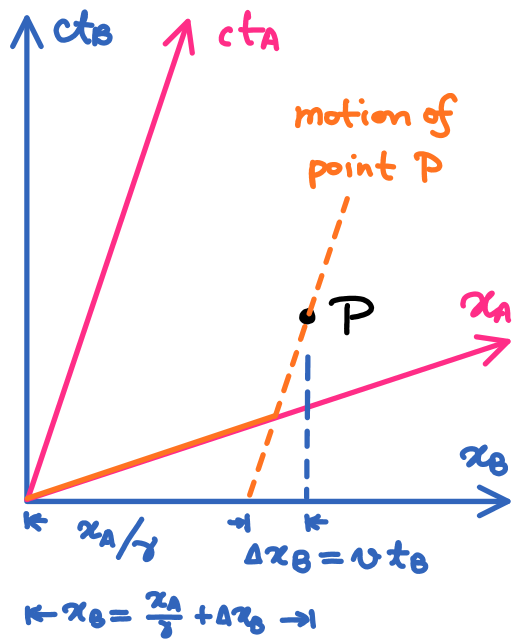
\includegraphics[width=\textwidth]{st_space_trans}
	}
	
	\tcblower

	如何获得 $t_B (t_A, x_A)$? 我们可以对掉 Alice 和 Bob 的角色并再次进行计算。 但实际上我们不必这样做。 简单地遵循 $(\mathbb{R})$,我们得到
	\begin{align}
		\label{eq:st_space_r}
		x_B = \gamma \left ( x_A + v t_A \right )~.
	\end{align}
}

\mtextbox{洛伦兹 vs 爱因斯坦}{
	洛伦兹变换因洛伦兹在 1892-1904 年间的工作而得名。 换句话说,洛伦兹变换在爱因斯坦的狭义相对论(1905 年)之前就已为人所知。 它被发现是麦克斯韦方程背后的数学对称性和解释 Michelson-Morley 实验的现象学方法。 但爱因斯坦首先了解了这种转变的物理原理。
}
\textbox{Time transformation of a boost}{\index{洛伦兹变换:时间}
	剩下的问题是:如何得到$t_A(t_B, x_B)$ 和$t_B(t_A, x_A)$? 我们不必做更多的思想实验,因为我们可以从方程 \eqref{eq:st_space} 和 \eqref{eq:st_space_r} 中求解它们。

	把 \eqref{eq:st_space} 代入 \eqref{eq:st_space_r} to 消去 $x_A$, 
	\begin{align}
	  \label{eq:stta}
	  x_B = \gamma \left [ \gamma \left ( x_B - v t_B \right ) + v t_A \right ]~.
	  \quad \rightarrow \quad
	  t_A = \gamma \left ( t_B - \frac{v}{c^2} x_B  \right )~.	  
	\end{align}
	类似地,或者简单地使用相对性原理,我们得到
	\begin{align}
	  \label{eq:stta_r}
	  t_B = \gamma \left ( t_A + \frac{v}{c^2} x_A  \right )~.  
	\end{align}
}

\mtextbox{洛伦兹对称性}{
	在变换的表象下,用一个更物理的名称来指代方程 \eqref{eq:ss-Lorentz}是洛伦兹对称:爱丽丝和鲍勃是对称的,尽管他们使用不同的坐标来描述事件,但他们遵守相同的自然规律(例如,粒子的运动方程)。 对称性现在被认为是基础物理学的第一原理。 我们将在作用原理部分回到对称性的概念。
}
\textbox{总结:洛伦兹变换}{\index{洛伦兹变换}
	让我们总结一下我们得到的转换,并添加回简单的 $y$ 和 $z$ 方向。 这些在惯性系之间变换的规则称为洛伦兹变换。 这里 $\beta \equiv v/c$.
	\begin{equation}
		\label{eq:ss-Lorentz}
		\left\{
		\begin{aligned}
			c t_A & = \gamma ( c t_B - \beta x_B) \\
			x_A   & = \gamma ( x_B - \beta c t_B) \\
			y_A   & = y_B \\
			z_A   & = z_B
		\end{aligned}
		\right.
		\qquad\qquad\qquad
		\left\{
		\begin{aligned}
			c t_B & = \gamma ( c t_A + \beta x_A) \\
			x_B   & = \gamma ( x_A + \beta c t_A) \\
			y_B   & = y_A \\
			z_B   & = z_A
		\end{aligned}
		\right.
	\end{equation}
}

洛伦兹变换描述了狭义相对论的数学结构。 因此,我们的已知结果可以直接从公式中得出 \eqref{eq:ss-Lorentz}.

\needspace{0.3\textheight}
\mtextbox{你tm为什么不早点告诉我们呀!}{你可能会在这里感到愤怒:
\mnewline
``我在理解时间膨胀、长度收缩和同时性的时候付出了巨大的努力。 但现在他们遵循如此简单的方程式。 你为什么不从告诉我们洛伦兹变换开始,然后从那里推导出一切? 那多省事儿呀。
\tcblower
事实上,我选择引入洛伦兹变换的时间点是经过深思熟虑的。
\mnewline
如果我之前介绍过,这些效果将只是你脑海中的冷酷无情的数学公式,而不是活生生的(即带有物理图像的)。
\mnewline
另一方面,我可以先教速度加法、能量和动量,然后将洛伦兹变换放在最后。 但是随后物理场景就会变得太复杂而无济于事。 因此,我选择现在作为介绍这个强大工具的时间点。
}
\textbox{重新审视时间膨胀、长度收缩和同时性}{
	\titem{
		\item 同时性:考虑两个事件 $E_1$ 和 $E_2$,同时发生在 Alice 身上,即 $t^{E_1}_A=t^{E_2}_A$。 Eq.~\eqref{eq:ss-Lorentz} 给出 $0=c(t^{E_1}_A-t^{E_2}_A) = \gamma [c (t^{E_1}_B-t^{E_2}_B )-\beta (x^{E_1}_B-x^{E_2}_B)]$。显然,如果这两个事件发生在不同的位置并且 $\beta\neq 为 0$,那么这两个事件不会同时发生在 Bob 身上。

        \item 时间膨胀:一个时钟在坐标为 $(t_A, 0)$ 的爱丽丝上移动。注意这里的 $x_A=0$ 因为 Alice 拿着时钟,因此时钟总是位于 Alice 的原点。从第一个方程到 \eqref{eq:ss-Lorentz} 的右面板,我们得到 $t_B = \gamma t_A$。

        \item 长度收缩:尺子与 Alice 一起移动。 Bob 应该如何测量它的长度? Bob 应该同时测量他在尺子两端的坐标。当 $t_B=0$ 时,标尺的左端位于 $x_B=0$。因此,$t_B=0$ 处的尺子坐标就是尺子的长度。从 \eqref{eq:ss-Lorentz} 左侧的第二个方程,我们得到 $x_B = x_A / \gamma$。
	}
}

现在我们准备解决一个问题:当 $v_A\sim c$ 时,牛顿速度加法规则 $\mathbf{v}_B = \mathbf{v} + \mathbf{v}_A$ 有什么问题? 在长度收缩部分的可选材料中,我们研究了一个特殊情况。 在这里,我们将推导出一般公式。

\textbox{速度加法}{\index{速度加法}
	为简单起见,让我们将沿 $x$ 方向的相对速度 $\mathbf{v}$ 设为 $(v, 0, 0)$,正如我们一直假设的那样。

	现在爱丽丝扔出一个球,速度为:
\begin{align}
  \label{eq:va}
  \mathbf{v}_A = (v_{Ax}, v_{Ay}, v_{Az}) 
  = \left( \frac{dx_A}{dt_A} , \frac{dy_A}{dt_A} , \frac{dz_A}{dt_A} \right)~.
\end{align}
Bob发现:
\begin{align}
  \mathbf{v}_B = (v_{Bx}, v_{By}, v_{Bz}) 
  = \left( \frac{dx_B}{dt_B} , \frac{dy_B}{dt_B} , \frac{dz_B}{dt_B} \right)~.
\end{align}
现在利用洛伦兹变换法则,可以计算出:
\begin{align}
  \label{eq:vbx}
  v_{Bx} = \frac{dx_B}{dt_B} 
  = \frac{\gamma d(x_A+v t_A)}{\gamma d\left(t_A + \frac{x_A v}{c^2} \right)}
  = \frac{dx_A+v dt_A}{dt_A + \frac{v}{c^2} dx_A} 
  = \frac{v_{Ax}+v}{1+\frac{v_{Ax}v}{c^2} }~.   
\end{align}
\begin{align}
  \label{eq:vby}
    v_{By} = \frac{dy_B}{dt_B} 
    = \frac{dy_A}{\gamma d \left ( t_A+\frac{v}{c^2} x_A \right )}
    = \frac{v_{Ay}}{\gamma \left(1+ \frac{v_{Ax} v}{c^2} \right)}~.  
\end{align}
类似地,
\begin{align}
  \label{eq:vbz}
  v_{Bz} = \frac{v_{Az}}{\gamma \left(1+ \frac{v_{Ax} v}{c^2} \right)}~. 
\end{align}
}

\textbox{例:垂直方向的速度相加}{
当$\mathbf{v}_A = (0, u, 0)$,垂直于相对运动方向,我们得到
	\begin{align}
	  \label{eq:vex}
	  \mathbf{v}_B = \left ( v, u/\gamma, 0 \right )~.
	\end{align}
	请注意,即使在垂直方向上,Alice 和 Bob 测量的速度也不同,因为它们的时间间隔不同(而长度间隔相同)。
}

\section{时空几何} \label{sec:geometry}

\textbox{毕达哥拉斯定理与现代几何}{
    自高斯和黎曼以来,数学家意识到不同类型的几何可以根据勾股定理在这些几何上出现的方式进行分类。 例如,在平面、球面和双曲曲面上,毕达哥拉斯定理的表现不同。
    \cg{0.7}{surf_geo}
    更仔细地研究球面和双曲面如何弯曲,可以使上述表达式更精确,并两次区分关系以定义空间曲率。
    \tcblower
    在这里,我们没有沿着这条路径深入研究纯空间几何。 相反,我们想问以下问题:既然空间和时间通过洛伦兹变换“统一”了,那么时空几何是什么样子的? 或者毕达哥拉斯定理对于时空是什么样子的?
}

\marginnote{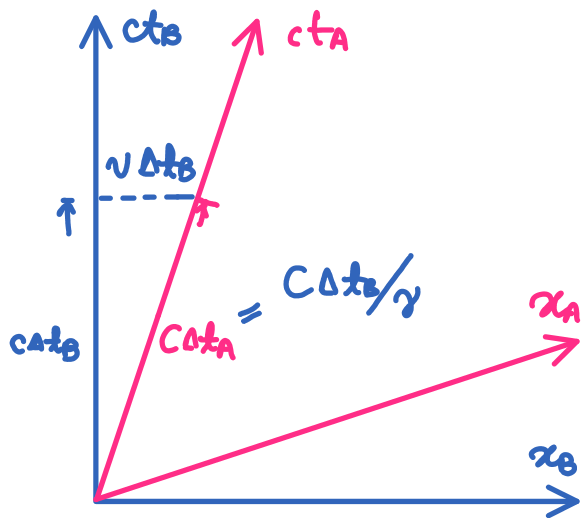
\includegraphics[width=0.3\textwidth]{st_geometry}}
\textbox{我们的时空不是欧几里得}{
    让我们重新考虑时间膨胀。爱丽丝带着一个时钟,爱丽丝和鲍勃都测量滴答间隔。

    写鲍勃,$\Delta t_B = \gamma \Delta t_A$。这在时空图上意味着什么?

    天真地,从几何上,我们会期望 $c\Delta t_A > c\Delta t_B$,因为 $c\Delta t_A$ 是直角三角形的斜边。然而,从 $\gamma>1$,我们看到 $c\Delta t_A < c\Delta t_B$。这怎么可能?

    正如我们所讨论的,我们不能认为欧几里得几何是理所当然的。
\marginnote{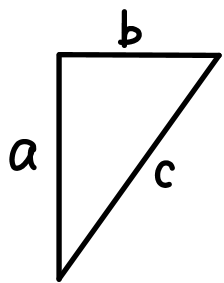
\includegraphics[width=0.1\textwidth]{st_right_tri}}
    特别是在右图中,$a$ 和 $c$ 是(Alice 或 Bob 的)时间方向,勾股定理 $a^2+b^2=c^2$ 不再成立。相反,对于时间膨胀,
	\begin{align}
	\label{eq:min_geo_tri}
	-a^2 + b^2 = -c^2 ~.
	\end{align}
	额外的减号出现在时间的平方前面,但不是空间。 \marginnote{请注意,时间平方的减号表示在时间前面有一个额外的因子 $i$ 以匹配平面空间的毕达哥拉斯定理。}

    这是巧合,还是一般来说是一种新的几何?
}

\mtextbox{双曲函数}{\index{双曲函数}
	$\cosh x \equiv \frac{e^x+e^{-x}}{2}$ \mnewline
	$\sinh x \equiv \frac{e^x-e^{-x}}{2}$ \mnewline
	$\tanh x \equiv \sinh x / \cosh x$ \mnewline
	$\cosh^2 x - \sinh^2 x = 1$ \mnewline
	$\cosh(i\theta) = \cos\theta$ \mnewline
	$\sinh(i\theta) = i \sin\theta$
}
\textbox{我们的时空几乎可以看作欧几里得时空}{\index{洛伦兹变换和旋转}
	用另一种方式看看发生了什么,让我们用速度 $\phi = \mathrm{arctanh}\beta$ 重写洛伦兹变换。 注意$\cosh \phi = \gamma$,并且$\sinh \phi = \beta \gamma$。 洛伦兹变换为
	\begin{equation}
		\left\{
		\begin{aligned}
			ct_B & =  ct_A \cosh\phi + x_A \sinh\phi \\
			x_B  & =  ct_A \sinh\phi + x_A \cosh\phi
		\end{aligned}
		\right.
	  \end{equation}
	你不觉得它有点像旋转吗?

	\tcblower

	现在让我们应用一个数学的小技巧。 定义
	\begin{align}
		\label{eq:theta}
		\phi \equiv i \theta ~, \qquad ct \equiv i w~.
	\end{align}
	然后我们得到
	\marginnote{不要问我此刻虚时间$w$的“物理意义”。 只需将其视为数学中的一个技巧。 事实上,虚时间在量子场论(零温度和有限温度)中有着深远的影响。 但我们还远远没有准备好在这里介绍它们。}
	\begin{equation}
	\label{eq:ss-Lorentz-Euclidean}
	\left\{
	\begin{aligned}
		iw_B & = (iw_A)\cos\theta + x_A(i\sin\theta) \\
		x_B  & = (iw_A)(i\sin\theta) + x_A \cos\theta
	\end{aligned}
	\right.
	\quad\Rightarrow\quad
	\left\{
	\begin{aligned}
		w_B & = w_A\cos\theta + x_A\sin\theta \\
		x_B  & = -w_A\sin\theta + x_A \cos\theta
	\end{aligned}
	\right.
	\end{equation}
	这是 \emph{exactly} $w$-$x$ 平面的旋转,$w$ 被视为额外的空间维度!

总结一下:重新定义变量的数学技巧使洛伦兹变换与旋转相同。
}

\textbox{时空的对称性与虚时间}{
	根据毕达哥拉斯(570BC-495BC)的说法,球体是最美丽、最完美的物体——它在 3 维旋转下是对称的。

	在这方面,我们的时空比最美丽的物体还要美丽。

    \marginnote{我们并不是说时空是一个球体。相反,球体是弯曲的,而我们的时空在狭义相对论中是平坦的。然而,它的对称性包括球体的对称性,甚至更多(还有 4 个额外的时空平移)。}

    这是因为,现在 $w, x, y, z$ 方向彼此没有区别——它们都是通过旋转相关的。在平面 $w$-$x$、$w$-$y$、$w$-$z$、$x$-$y$、 $x$-$z$、$y$-$z$,以及它们的各种组合。它确实比球体更对称,因为球体仅在 $x$-$y$、$x$-$z$、$y$-$z$ 平面及其组合中的旋转下是不变的。

    这进一步证实了空间和时间之间的差异是虚构的——一旦你使用虚构的时间,时间就变得与另一个空间方向没有区别,沿 $x$、$y$ 和 $z$ 方向的3个推动只是变成了三个额外的旋转。
}

\textbox{自然单位——自然的单位}{
	在物理学中,一些单位比其他单位更自然,因为它们对相同的事物使用相同的单位(或明显不同的事物,但具有相同的物理起源)。
	
	\marginnote{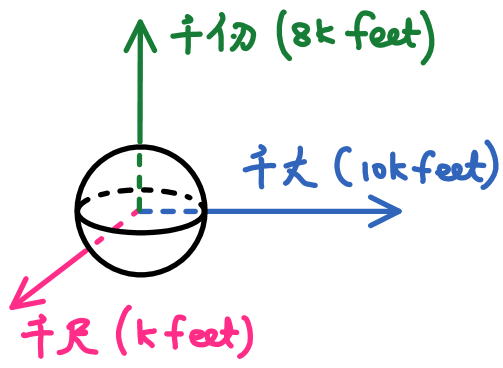
\includegraphics[width=0.3\textwidth]{natural_unit_rot}}
	让我们考虑一个不太自然的单位的例子。 在中国古代,有时人们用不同的单位来表示山的高度。 那时,高度似乎与其他方向不同,因为重力。 但现在我们看到,差异是由于地球的存在,它自发地打破了空间的对称性。 从根本上说,高度与其他两个方向没有区别,它们可以通过旋转关联起来。 因此,我们最好使用相同的单位来测量高度和其他空间维度。

	\mtextbox{自然的 vs 方便的}{
		由于避免了不必要的单位转换,自然单位制的自然规律更短。 然而,这种单位的选择是否方便取决于我们研究的物理环境。 如果我们用 $v\ll c$ 研究确切的系统的动力学,那么我们最好在式子中确切的保留 $c$ ,否则我们将到处处理过大/过小的数。 例如,对于 $v=10^{-8}c \simeq 3$m/s,在自然单位中,物体在一个单位时间内仅移动 $10^{-8}$ 个单位空间。
	}

	\tcblower

	现在我们已经看到空间和时间并不是完全不相关的,并且可以通过洛伦兹变换关联起来,为什么我们还要给空间和时间赋予不同的单位呢? 我们其实不必这样做。

	要使用相同的空间和时间单位,我们可以设置 $c=1$,即速度是无量纲的。

    这被称为自然单位(与 $\hbar=k_B=1$ 一起)。 自然单位在理论高能物理中被广泛使用。

    我们不会在这里使用自然单位,并且将始终保持 $c$ 是确切的。
}

\textbox{不变区间}{\index{不变区间}\index{四维矢量}\index{闵可夫斯基時空}

	在欧几里得时空里, 
	\begin{align}
	\label{eq:dse}
	ds^2 = dw^2 + dx^2 + dy^2 + dz^2~.
	\end{align}
	回想 $w=-ict$。带回真正的时间, 因此我们得到
	\marginnote{在某些书中,区间定义为 $ds^2 = d(ct)^2 - dx^2 - dy^2 - dz^2$。 这只是一个没有物理差异的不同约定(对应将这里的所有$ds^2$替换为$-ds^2$)。}
	\begin{align}
	\label{eq:dsl}
	ds^2 = - d(ct)^2 + dx^2 + dy^2 + dz^2~.
	\end{align} 
	$ds^2$ 的重要性在于,它是洛伦兹变换下的不变量。 要看到这一点,可以首先使用 $\{w, x, y, z\}$ 并注意旋转保持半径不变。 或者可以使用洛伦兹变换矩阵来明确地验证它。 正如 $(\omega, x, y, z)$ 在四维欧几里得空间中形成一个向量,$x^\mu = (ct, x, y, z)$ ($\mu=0,1,2,3 $) 也形成一个 4 维向量(简称 4-vector),它存在于所谓的 \emph{闵可夫斯基时空} 中——这只是我们时空的数学名称。 \marginnote{事实上,我们的时空比闵可夫斯基空间更复杂——在广义相对论中,你会看到我们的时空是弯曲的,而不是完全平坦的。 这被认为是更一般的时空,但仍带有一些闵可夫斯基的迹象。}

	\tcblower 

	事实上,“相对论”并不是该理论的好名字。 顾名思义,它似乎强调事物是相对的——不再像我们想象的那样一成不变。
	
    但实际上,相对论的本质是相反的:尽管从不同的角度来看(不同的观察者在不同的惯性参考系中),但事件及其内在关系是不变的。
	\marginnote{
		回忆一下 $(\mathbb{R})$、$(\mathbb{C})$ 和 $(\mathbb{E})$ 的原理。 每一个原则都告诉你一个不变性,而不是相对性。回忆一下 $(\mathbb{R})$、$(\mathbb{C})$ 和 $(\mathbb{E})$ 的原理。 每一个原则都告诉你一个不变性,而不是相对性。
		\mnewline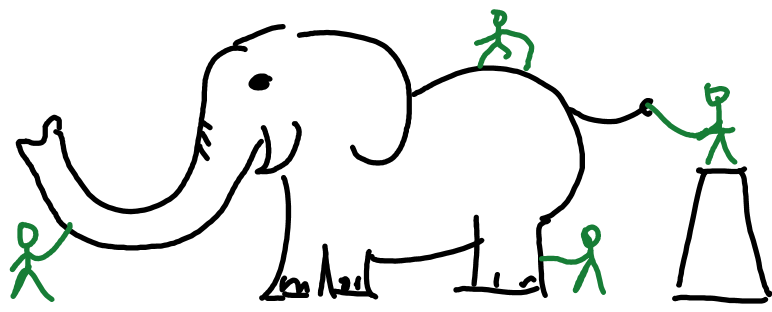
\includegraphics[width=0.42\textwidth]{touch_elephant}}
	相对论只是研究的技术。 但该理论的精神是潜在的不变性。 

	这就像您如何证明欧几里得几何中的定理一样——图形是垂直放置还是水平放置(即具有不同视角的观察者)并不重要。 重要的是几何对象之间的内在关系。

    另一个类比是盲人和大象的故事。 物理学的目标是了解大象,而不是因为无法感受整个事物而对不同人产生的不同的感受。
    }

\textbox{类时、类空和零的区间}{
	$ds^2$ 的符号对应于不同类型的事件分离:
	\begin{align}
		\label{eq:tsn}
		ds^2 < 0 &\quad\Leftrightarrow\quad \mbox{类时} \nonumber\\
		ds^2 > 0 &\quad\Leftrightarrow\quad \mbox{类空} \nonumber\\
		ds^2 = 0 &\quad\Leftrightarrow\quad \mbox{类光, 零}~.  
	\end{align}
	\tcblower
	现在您知道为什么零被称为零了——它确实是零。 
}

\mtextbox{(选读)四维向量的内积}{
	不变的内部$ds^2$ 可以认为是四维向量$dx^\mu$ 与自身的内积。 一般来说,我们可以使用度量内积来衡量任何4个向量的内积。 对于两个四维向量 $p^\mu$ 和 $k^\nu$,它们的内积 $\sum_{\mu\nu}g_{\mu\nu}p^\mu k^\nu$ 是洛伦兹不变量 (即在洛伦兹变换下不变)。
}
\textbox{(选读) 时空度规}{\index{度规}
	度规是测量坐标距离的“标准”。 对于狭义相对论中的时空,度规 $g_{\mu\nu}$(作为对称的 $4\times 4$ 矩阵)、无穷小的坐标距离和不变区间可以关联为
	\begin{align}
		\label{eq:dsg}
		ds^2 = \sum_{\mu,\nu=0}^3 g_{\mu\nu} dx^\mu dx^\nu~,	  
		
	\end{align}
	此处,
	\begin{align}
	\label{eq:defg}
	x^\mu=\{ct, x, y, z\}~, \qquad g_{\mu\nu} = 
	\left( \begin{array}{cccc}
		-1 & 0 & 0 & 0 \\
		0 & 1 & 0 & 0 \\
		0 & 0 & 1 & 0 \\
		0 & 0 & 0 & 1
	\end{array} \right)~.
	\end{align}
	这似乎是对我们所获得的内容的微不足道的重写。 但是,在这里我们分离了两个不同的东西:
	\begin{itemize}
		\item 坐标 $x^\mu$: 时空的方向是什么?
		\item 几何: 时空满足怎样的几何?
	\end{itemize}

	即使我们使用一个不同的坐标体系, 
	\marginnote{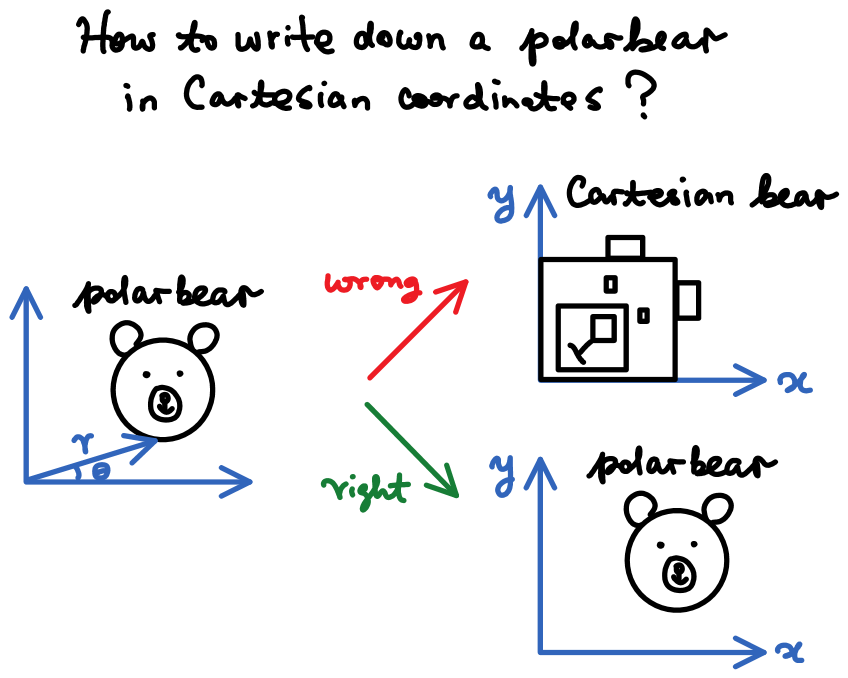
\includegraphics[width=0.3\textwidth]{polarbear}}
	for example, spherical coordinate for the spatial part, we can still choose a metric to keep $ds^2$ invariant:
	\begin{align}
		x^\mu=\{ct, r, \theta, \phi\}~, \qquad g_{\mu\nu} = 
		\left( \begin{array}{cccc}
			-1 & 0 & 0 & 0 \\
			0 & 1 & 0 & 0 \\
			0 & 0 & r^2 & 0 \\
			0 & 0 & 0 & r^2 \sin^2\theta
		\end{array} \right)~.
	\end{align}
	
	\tcblower

	事实上,度规所带来的优势不仅仅是可以自由选择坐标。 它还可以描述时空的内在曲率,且这种曲率并不因不同的坐标系而不同。 但这超出了狭义相对论的范围。 稍后您将看到,在广义相对论中,度规 $g_{\mu\nu}$ 是最重要的研究对象。 它可以被物质弯曲,并且可以引导物质如何运动。
}

\section{相对能量和动量}\label{sec:momentum-energy}


\mtextbox{Transforming Slimes}{
	Consider the following quiz: 
	\mnewline
	Suppose there are slimes of 3 shapes: $\triangle$, $\square$ and $\ocircle$. When slimes of differt shapes meet, they transform into the third shape. For example:
	$$
	\triangle + \square \rightarrow \ocircle \times 2 ~.
	$$
	Now that we have $\triangle\times 5$, $\square \times 7$ and $\ocircle \times 9$. Can you let them meet and transform them into $\triangle\times 6$, $\square \times 7$ and $\ocircle \times 9$ ?
	\mnewline
	Obviously not. Since the total number of slimes is conserved when they meet.
	\mnewline
	Fine. So, what about we have $\triangle\times 5$, $\square \times 7$ and $\ocircle \times 9$. Can you transform them into $\triangle\times 6$, $\square \times 9$ and $\ocircle \times 6$ ? 
	\mnewline
	Not either. Note that $(\#\triangle - \#\square) ~ \mathrm{mod} ~ 3$ is also conserved (where $\#$ denotes ``number of''). Which is violated.
	\tcblower
	Hope you get some feeling here that conserved quantities are helpful.
}
在讨论相对论中的能量和动量之前,让我们首先回顾一下为什么我们需要它们。 在牛顿力学中,有能量和动量是很好的,因为它们是守恒的。 (看下面的补充说明,了解为什么守恒定律总是好的。)因此在相对论中,我们应该检查牛顿对能量和动量的定义是否仍然守恒; 如果不是,如何推广能量和动量的定义,使它们仍然守恒。

\textbox{守恒定律有什么好的?}{\index{守恒定律的重要性}
	\titem{
		\item 从物理上讲,守恒定律让我们不需要关心中间发生了什么的魔法。 给定初始状态,我们可以立即做出一些预测(不超过系统中守恒定律的数量)。

		\item 在数学上,运动方程(如一组 $m \ddot x + V'=0$)是 $x$ 的二阶常微分方程(ODE),这可能很困难。 守恒定律将其中一些转换为 $x$ 的 1 或 0 阶 ODE,这就简单得多(例如 $\frac{1}{2} m\dot x^2 + V = E$,或电荷守恒)。

		\item 实际上,在现代物理学中,被研究的物体通常非常快($v\sim c$),小($\Delta x\times \Delta p \sim \hbar$),重($GM/(rc^2 ) \sim 1$)、早(大爆炸后不到一秒)等。通常很难直接建立实验来直接监控正在发生的事情。 人们通常需要守恒量来进行有用的观察。 例如,在大型强子对撞机等现代对撞机上,与发生相互作用的时间相比,研究粒子的轨迹(在上述意义上它们都既小又快)的时间要晚得多。 如果电荷、能量或动量不守恒,那么研究这样粒子的物理过程就会变得更加困难(事实上,如果没有能量和动量守恒的帮助,理论上如何定义可观测量也将变得不清楚)。
	}
	\tcblower
	这很酷。 但是为什么我们因狭义相对论中有能量和动量守恒感到幸运呢? 在后面的《从作用用量到自然法则》中,我们会给你一个正面的答案——这些守恒定律的存在不是运气的结果,而是没有时间和空间位置是特殊的的结果。  这适用于狭义相对论以及牛顿力学。 如果你对这些守恒定律的起源感到好奇,请等待学习那部分的内容。
}

\subsection{相对动量}

\textbox{我们还可以使用牛顿力学中的动量守恒吗?}{\index{动量:为什么不是牛顿力学}
	首先,让我们回顾一下牛顿力学中的动量守恒如何与牛顿力学中的 $(\mathbb{R})$ 一致——暂时忘记相对论并假设 $v\ll c$。

	例如,对于 Alice 的两个粒子的动量守恒:
	\begin{align}\label{eq:momentum_conservation}
		m_1 \mathbf{v}_1^A + m_2 \mathbf{v}_2^A = m_1 \mathbf{v}_1'{}^A + m_2 \mathbf{v}_2'{}^A~.
	\end{align}
	鲍勃会发现什么? 在牛顿力学中,粒子的质量不会改变。 速度只是增加了。 因此对于具有相对速度$\mathbf{v}$的 Bob
	, $\mathbf{v}_1^B = \mathbf{v}_1^A +\mathbf{v}$,其余速度同理。 因此,在鲍勃的参考系里,等式 \eqref{eq:momentum_conservation} 始终可以被写成一样的形式。
	\begin{align}
		m_1 \mathbf{v}_1^B + m_2 \mathbf{v}_2^B = m_1 \mathbf{v}_1'{}^B + m_2 \mathbf{v}_2'{}^B~.
	\end{align}
	令人高兴的是,所有带有 $\mathbf{v}$ 的项都在上面的等式中消掉了。 所以它采用与 \eqref{eq:momentum_conservation} 相同的形式。 因此,($\mathbb{R}$) 确实是满足的。
	  
	\tcblower

	现在,让我们考虑相对论。 为简单起见,让我们断言粒子的质量仍然不随速度变化。 \emph{假设} Alice 仍然有动量守恒方程 \eqref{eq:momentum_conservation},那么 Bob 会发现什么?

	\mtextbox{当质量取决于速度的时候怎么办}{我们确实可以假设质量取决于速度。 我们将得到基本相同的相对论动量,只是质量的定义不同,即所谓的“相对论质量”:$m_{\mathrm{rel}} = \gamma m$。 在这里我们不会使用这种记法。}

	遵循速度加法规则,Bob 发现(我们只明确写出第一个粒子的式子以强调关键)。 让 Alice 和 Bob 之间的相对速度像往常一样沿着 $x$ 方向。 然后在 $x$ 方向,我们有:
	\begin{align}\label{eq:mom-wrong1}
		m_1 \frac{(v_{1Ax}+v)}{{\color{red}  (1 + \frac{v_{1Ax}v}{c^2} )}}  + \cdots
		=
		m_1 \frac{(v'_{1Ax}+v)}{{\color{red} (1 + \frac{v'_{1Ax}v}{c^2} )}} + \cdots ~.
	\end{align}
	在 $y$ 方向($z$ 方向的方程同理),我们有:
	\begin{align}\label{eq:mom-wrong2}
		m_1 \frac{v_{1Ay}}{{\color{red}\gamma (1+ \frac{v_{1Ax}v}{c^2} )}} + \cdots 
		= 
		m_1 \frac{v'_{1Ay}}{{\color{red}\gamma (1+ \frac{v'_{1Ax}v}{c^2} )}} + \cdots ~.
	\end{align}
	令人失望的是, 
	\marginnote{这种想法同样也适用于牛顿力学的能量。}
	由于式子中里红色的因子,这些方程 \emph{不} 采用与 \eqref{eq:momentum_conservation} 相同的形式。 因此,\eqref{eq:momentum_conservation} 相对于 Alice 和 Bob 是不同的。 它不可能是狭义相对论中的一条自然法则。
}

\marginnote{事实上,我们只需要在在 $v\ll c$ 时的能量和动量 \emph{差} 就可以回到牛顿力学。 你很快就会在这方面发现有关能量的惊喜。}

现在我们已经知道牛顿力学里的能量和动量不是守恒量(以及没来由的坚信存在守恒能量和动量),我们能做的最好的事情就是在狭义相对论中寻找新的量,其中 $ v\ll c$ 限制了牛顿力学中能量和动量。

\needspace{0.3\textwidth}
\mtextbox{固有时间的物理意义}{
	为什么时间变量可以定义为\emph {独立于}观察者的? 我们不是说过没有绝对的时间吗?
	\tcblower
	因为存在一个运动的物体。 移动对象定义了自己的参考系,从而定义了自己的时间。 在运动物体自己的参考系中,$d\mathbf{x}=0$。 因此确实$d\tau = dt$。 这验证了正确的时间是移动物体本身测量的时间。 想象一个时钟与物体一起移动。 正确时间是从此时钟读取的时间间隔。
}
\textbox{使用固有时间来使动量守恒成立}{\index{动量}\index{固有时间}
	如何修复 \eqref{eq:mom-wrong1} 与 \eqref{eq:mom-wrong2} 和 ($\mathbb{R}$)的不一致?

	如果我们可以去掉红色因子,我们就应该能得到一个满足 ($\mathbb{R}$) 的方程。 如何实现? 我们知道红色的因子出现是因为
	\begin{align}
		dt_B = d \left[ \gamma \left( t_A + \frac{x_A v}{c^2} \right) \right] = \gamma (1+ \frac{v_{1Ax}v}{c^2} ) dt_A~.
	\end{align}
	
	换句话说,每个观察者都有自己的时间。 用独立的观察者自己的时间测量运动($d(\cdots) / dt_A$ 和 $d(\cdots)/dt_B$)是万恶之源。

	我们如何才能摆脱观察者自己的时间定义动量? 或者,是否有一种独立于观察者的方法来测量类时间间隔?
	
	当我试图重新表述问题以接近答案时,你应该能够弄清楚:我们已经学会了一种独立于观察者的方法来使用 $ds^2$ 测量间隔。 为了得到一个具有正确时间维度的实数,我们定义了 \emph{固有时间}:
	\begin{align}
		d\tau \equiv \sqrt{ - ds^2 /c^2} = \sqrt{dt^2 - \frac{dx^2}{c^2} } = \frac{dt}{\gamma}~. 
	\end{align}
	这是我们需要的时间变量。 因此,实现动量守恒的在相对论中的一般化的动量是
	\begin{align}
		\label{eq:ptau}
		\mathbf{p} = m \frac{d \mathbf{x}}{d\tau} 
		= \gamma m \mathbf{v}~. 	  
	\end{align}
	\tcblower
	从方程 \eqref{eq:ptau} 的第一个等号可以看出,$\mathbf{p}$ 的变换方式与洛伦兹变换下的 $\mathbf{x}$ 相同。 正如所承诺的那样,动量守恒在不同的参考系中采用相同的形式。

    然而,这从另一个方面来说是令人困惑的:我们知道空间 ($\mathbf{x}$) 和时间 ($ct$) 在相对论中作为一个实体组合成时空 $(ct, \mathbf{x})$。 现在动量变换与空间相同,是否存在与时间相同的对应物($ct$)? 如果我们在 \eqref{eq:ptau} 中天真地将 $\mathbf{x}$ 替换为 $ct$,我们会得到什么? 我们得到
	\begin{align}
		\label{eq:p0tau}
		\mbox{(类时间的对应物)}\mathbf{p})
		= m \frac{d(ct)}{d\tau} = \gamma m c~. 
	\end{align}
	这是什么? 大自然绝不应该让它无法解释! 我们将在下一小节中回到这个问题。
}

注意:这里我们只展示了定义 \eqref{eq:ptau} 与 $(\mathbb{R})$ 是一致的。 我们还没有为你证明实际的守恒。 在牛顿力学中,动量守恒源自第三定律(这是牛顿第一和第二定律的独立假设)。 在这里,我们没有使用第三定律(尽管我们可以这样做),因此我们没有正确的工具来推导动量守恒。 事实上,给定一个作用量,相对论动量守恒可以从一个作用量原理推导出来。 我们不会在这里展开这一点。

\textbox{相对论中的李}{\index{力}
	现在有了动量,就直截了当地\marginnote{这里我们用$dt$代替$d\tau$。 这个定义很方便,因为可以直观地将力想象为一个静态观察者推动一个物体并看到它的加速度——静态观察者必须消耗多少额外的努力才能将火箭推得更远。} 定义力:
	\begin{align}
	\label{eq:force}
	\mathbf{F} \equiv \frac{d \mathbf{p}}{dt} = \frac{d (\gamma m \mathbf{v})}{dt} = \gamma m \dot{\mathbf{v}} + \gamma^3 m \mathbf{v} (\mathbf{v} \cdot \dot {\mathbf{v}}) / c^2~. 
	\end{align}

	注意当$v\rightarrow c$ 时,需要$F\rightarrow \infty$ 来改变$v$。 因此,人们永远无法将速度趋近于光速的物体加速到光速(或更高的速度)。 因此 $c$ 确实是速度上限。
    \mtextbox{追光?}{爱因斯坦 16 岁时,他开始梦想如果他能像光跑的一样快会发生什么。 光会停止振荡吗?这会与麦克斯韦的 E\&M 理论相矛盾吗?
    \tcblower
    现在他的梦想已经落幕了。 没有人可以加速到光速,因此这个看似矛盾的思想实验永远不会发生。}
}

\subsection{相对能量}

\textbox{相对动能}{
	相对论力意味着使物体加速的功,因此也意味着动能。 考虑一个初始位置为 $x=0$ 的静止物体,并受 $x$ 方向上的力加速,进入位置 $x$ 和速度 $v$ 的状态。 力所做的功转化为物体的动能:
	\begin{align} \label{eq:ek}
		K = \int_0^x F ~ dx = \int_0^x \frac{d(\gamma m v)}{dt} ~ dx = \int_0^v v ~ d(\gamma m v) = (\gamma-1)mc^2~.
	\end{align}  
	在倒数第二步中,我们将积分变量转换为 $v$,在最后一步中,我们进行了分部积分。 细节留作练习。
	\tcblower
	在继续下去前的一些批注:
	\titem{
		\item 当 $v\ll c$ 时(这样我们可以在 $v\rightarrow 0$ 处进行泰勒展开),相对论动能按预期回到到我们熟悉的牛顿形式:$K\rightarrow \frac{1}{2} mv^2$。
		\item 我们已经讨论了从静止开始沿 $x$ 方向加速后的动能。 这够普适吗? 由于动能是一个状态量,它不应该关心是如何从物体的历史过程中获得的。 因此,无论力不在 $x$ 方向上,或者物体是否具有初始速度,动能都足够普适。
	}


}

现在我们有了动能,那么总能量是多少? 在此之前,让我们先研究一下质量。 在牛顿力学(和化学)中,质量是守恒的——反应前后的总质量是相同的。 那在相对论中呢?
\needspace{0.2\textheight}
\mtextbox{ $v_y$ 变化吗?}{	
	不,因为我们可以在另一个参考系中以 $v_y=0$ 的初始状态查看事件。 然后在这个参考系 $v_y=0$ 结束。 现在切换到一个带有小 $v_y\ll c$ 的框架。 使用速度加法规则,$v_y$ 不会改变。 (并且在 $x$ 方向 $v_x$ 只得到一个小的修正 $1/\sqrt{1-v_y^2/c^2}-1 = \mathcal{O}(v_y^2/c^2)$.)
}
\textbox{质量不再守恒}{\index{质量:不守恒}
	我们研究一个分成两个对象的系统。 考虑通过弹簧连接的两个物体。 弹簧被压缩并储存一些势能。 最初,两个物体都处于静止状态。 整个系统的初始质量为$M$。 释放弹簧后,两个物体分开,每个物体的质量为 $m$,并以 $v$ 的速度分开。

	\cg{0.5}{e-split} 
	
	在牛顿力学中,
	 $M=2m$是无可置疑的。但是当 $v\sim c$时还成立吗?

	\tcblower

	为了研究系统的性质,
    我们在 $y$ 方向 $v_y \ll v$ 上添加一个小的试探速度(可以简单的将 $v_y$ 设为无穷小)。 然后有趣的是,$y$ 方向的动量守恒可以为我们计算 $M$。

	\titem{
		\item 分开之前: $p_y = M v_y$.
		\item 分开之后: $p_y = 2\gamma m v_y$ 对于相同的 $p_y$ (动量守恒),其中 $\gamma = 1/\sqrt{1-v^2/c^2}$ 不仅考虑了 $y$ 方向的速度,还考虑了总速度。
	}

	因此,$M=2\gamma m > 2m$! 曾经的质量守恒被打破了。
}

\textbox{相对静止质量}{
	考虑上面的 $M\rightarrow 2m$ 拆分过程。 让我们考虑一下极限 $\gamma \gg 1$,即最终物体的飞行速度非常接近光速。 在这个极限下,最终物体的动能是$K\simeq 2\gamma m c^2$。
    \marginnote{最后两个物体也有每个 $mc^2$的静止能量。 在我们的 $\gamma\gg 1$ 限制中,这些静能可以忽略不计。 事实上,最初爱因斯坦使用光来导出相对论能量,对应于没有静止质量。 但是推导需要更多超出本课程的电磁学知识。 因此,我们在这里选择走另一条路。}

    从能量守恒来看,最终物体的动能包含在初始物体中。 因此,初始物体的能量为
	\begin{align} 
		E = 2\gamma m c^2 = M c^2. 
	\end{align}
	回想一下,初始对象是静止的。 因此,这里的能量是物体的静止能量。
	\tcblower
	\index{静止能量}
	\mtextbox{香港每日能源消耗}{为了理解物质巨大的静止能量,举个例子,香港每日能源消耗量为$10^{15}$J. 这相当于大约 $10$ 克的物质——大约是一节 AAA 电池的重量。 相比之下,一节 AAA 电池所能提供的化学能是几千焦耳。}
	静止能量
	\begin{align} \label{eq:e0}
		E_\mathrm{rest} = mc^2	
	\end{align}
	是物体具有的能量的一部分,即使它根本没有移动。 这种能量在我们的日常标准中是巨大的,因为 $c$ 在我们的日常生活中是一个巨大的数字(而在能量里我们有 $c\times c$)。

    在牛顿力学中,由于质量守恒,在能量守恒中没有注意到这种能量。 然而,在相对论的情况下,这种能量可以被释放。 例如,

    \mtextbox{星星为什么会发光?}{在理解相对论之前,如果星星是由化学能驱动的,那么星星如何发光的时间比人类历史还要长,这是一个很大的谜团。 而恒星中的核聚变就可以为恒星提供数十亿年的动力。}
	\titem{
		\item 我们已经在上面遇到了一个并不显然的的静止能量案例——分开后的两个最终对象具有 $E=M c^2 > 2mc^2$。
        \item 在更现实的情况下,核能的使用利用了物质的剩余能量。 核裂变和聚变与通常的化学或机械反应相比,可以释放更多的能量。
        \item 在实验室中,可以碰撞粒子和反粒子。 粒子相遇后消失,剩下的能量可以完全以光的形式释放出来。
		 
	}	
}

\mtextbox{静止能量的零点}{粒子-反粒子湮灭现象是对静止能量概念的一个非常重要的检验。 因为能量的零点没有物理意义,除非所有的能量都可以释放。}
\textbox{相对论能量}{\index{能量}
	一般来说,对于质量为$m$、速度为$v$的物体,结合动能\eqref{eq:ek}和静止能量\eqref{eq:e0},物体的总能量为
	\begin{align} \label{eq:relei}
		E = \gamma m c^2 ~.
	\end{align}
	\tcblower
	这似乎和你听到的有点不同:$E=mc^2$。 这个更著名的公式(之所以著名是因为不必在科普中解释$\gamma$)可能代表以下两种含义之一:
	\titem{
		\item 物体的静止能量
		\item 物体的总能量,其质量定义为与速度相关的“相对论质量”$m_\mathrm{rel} \equiv \gamma m$,因此 $E=m_\mathrm{rel} c^2$ . 如今,我们将质量理解为粒子洛伦兹变换的不变量。 $m_\mathrm{rel}$ 的约定很少使用,因此我们不会在这里进一步使用 $m_\mathrm{rel}$。
	}
}

\needspace{0.2\textheight}
\mtextbox{光就是光}{
	将 \eqref{eq:mep} 应用于光,我们有 $v=c$。 因此,$m=0$。 换句话说,如果我们将光视为粒子(有关更多信息,请参阅量子力学部分),它们的质量必须消失。
    \tcblower
    光动量的 四维矢量具有 $p^\mu = (E/c, \mathbf{p})$ 的形式,其中光的能量 $E = c |\mathbf{p}|$。 这个四矢量在闵氏空间的意义下长度为零。 在度规的记法中(选读)中,我们有 $\sum_{\mu, \nu} g_{\mu\nu}p^\mu p^\nu=0$。
}
\textbox{四维动量矢量}{\index{四维动量}\index{不变质量}
    还记得我们在 \eqref{eq:p0tau} 提出的问题吗? 幸运的是,多达 $c$ 的因子(这只不过是我们解释自然单位的单位转换),我们在 \eqref{eq:relei} 中获得的能量正是缺失的“朴素时间- 就像 \eqref{eq:p0tau} 中的相对动量''。 那么四维动量矢量是 $p^\mu = (E/c, \mathbf{p}) = (\gamma mc, \gamma m\mathbf{v}) = \gamma m \dot x^\mu$。

    回想一下,对于时空坐标四维向量,我们有一个不变量 $c^2 \Delta t^2 - \Delta x^2$。 动量 4 向量是否有对应物? 是的。 平方方程~\eqref{eq:relei},我们得到
	\begin{align}\label{eq:mep}
		m^2 c^4 = E^2 - \frac{v^2}{c^2} E^2	= 
		\xlongequal{\mbox{using ratio of \eqref{eq:relei} and \eqref{eq:ptau}}}
		E^2 - p^2 c^2~.
	\end{align}
	Thus, though $E$ and $\mathbf{p}$ are dependent on observers, the combination on the RHS is independent of observers, but is just the invariant mass squared of the particle. This is not surprising. Because the momentum and coordinate 4-vectors lives in the same space and is measured by the same metric. (Just as it is not surprising that both the magnitude of 3d coordinate vector and 3d momentum are rotational invariant.)
}

\textbox{(Optional) The relativistic Doppler effect of light}{
	Alice is moving with 3-velocity $\mathbf{v}$ wrt Bob. If Bob observes that the energy of light is $E_B$, what's the corresponding energy $E_A$ of the same beam of light in Alice's frame?

	We can solve this problem by the Lorentz invariance of inner products of 4-vectors. The inner product $\sum_{\mu\nu}g_{\mu\nu}k^\mu p^\nu$ is invariant under Lorentz transformations, where $k^\mu$ and $p^\nu$ are the 4-vector of Alice's momentum and the momentum of the beam of light.

	In Bob's frame: $k^\mu = (\gamma m c, \gamma m \mathbf{v})$, $p^\nu = (E_B/c, \mathbf{p})$. The Lorentz invariant inner product is $\sum_{\mu\nu}g_{\mu\nu}k^\mu p^\nu = -\gamma m (E_B-\mathbf{v}\cdot\mathbf{p})=-\gamma m E_B (1 - (v/c) \cos\theta)$, where $\theta$ is the angle between $\mathbf{v}$ and $\mathbf{p}$ in Bob's frame.

	In Alice's frame: $k^\mu = (mc, \mathbf{0})$, $p^\nu = (E_A/c, \mathbf{p'})$. The Lorentz invariant inner product is $\sum_{\mu\nu}g_{\mu\nu}k^\mu p^\nu = - m E_A$. It must be equal to the Lorentz invariant in Bob's frame. Thus, $E_A = \gamma E_B (1 - (v/c) \cos\theta)$. 
	\tcblower
	From 
	\marginnote{Here the purpose of this optional box is not only to tell you the formula of the relativistic Doppler effect, but also to show the power of Lorentz invariance for the inner product. The Doppler effect can also be derived just by considering the effect of time dilation and space contraction. But the calculation is much more complicated for a general direction $\theta$.}
	either classical E\&M or quantum mechanics, we will find that the frequency of light is $\omega \propto E$. Thus the frequency of light wrt Alice and Bob has a similar relation $\omega_A = \gamma \omega_B (1 - (u/c) \cos\theta)$.
}

\section{Epilogue: Summary and What's Next}

The below diagram is a recap of what we have learned. The green color denote external contents (you may ignore) and the blue denote alternative logic.

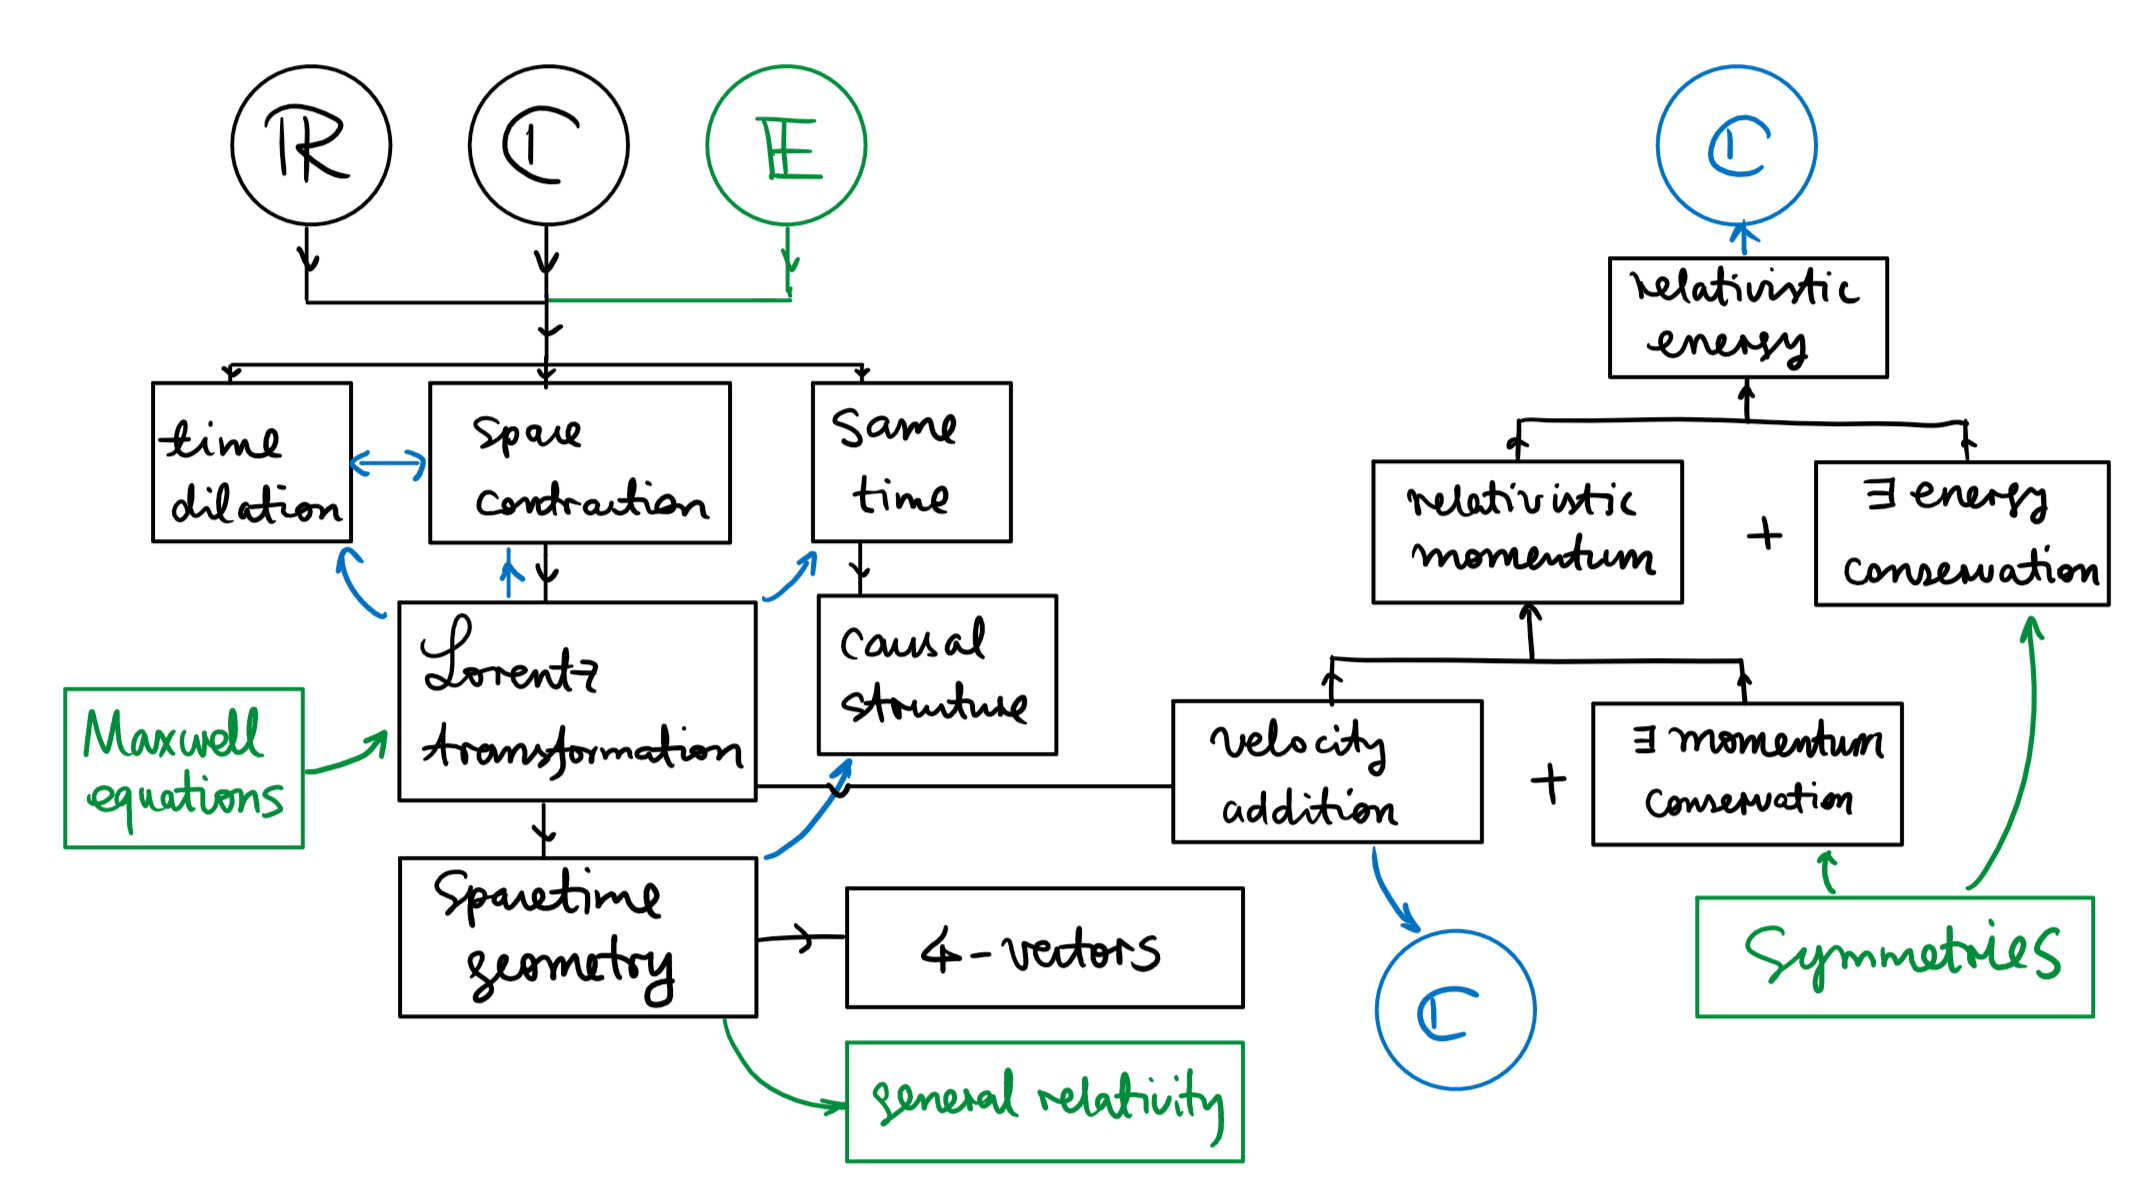
\includegraphics[width=1.3\textwidth]{summary_relativity}

\textbox{Further reading about the content}{
	\titem{
		\item If you are interested to explore more about the geometry of spacetime and formulate special relativity with geometrical emphasize, read \href{https://www.amazon.com/Spacetime-Physics-Edwin-F-Taylor/dp/0716723271}{``Spacetime Physics''} by Taylor and Wheeler (and the a few general relativity books below).
		\item If you are not happy about our guess of relativistic energy and momentum, but rather want to derive them, wait and we will do it in the part ``From Action to Laws of Nature''. See also \href{
			http://theoreticalminimum.com/}{``Theoretical Minimum'' (Video Lectures)} by Susskind.
		\item If you consider the math used this text too sloppy, read \href{https://www.amazon.com/Relativity-Special-Cosmological-Wolfgang-Rindler/dp/0198567324}{``Relativity: Special, General, and Cosmological''} by Rindler.
		\item If you like to learn more about the relation between electrodynamics and relativity before getting to the full details of electrodynamics, read \href{
			http://www.damtp.cam.ac.uk/user/db275/concepts/Concepts.pdf}{Lecture Notes on Modern Physics} by Baumann.
		\item Many good books on general relativity also starts with a dense and high-level introduction of special relativity, for example \href{https://www.amazon.com/Gravity-Introduction-Einsteins-General-Relativity/dp/0805386629}{Gravity: An Introduction to Einstein's General Relativity} by Hartle, \href{https://www.amazon.com/Gravitation-Charles-Misner/dp/0691177791}{Gravitation} by Misner, Thorne and Wheeler and \href{https://www.amazon.com/Gravitation-Cosmology-Principles-Applications-Relativity/dp/8126517557}{Gravitation And Cosmology} by Weinberg.
	}
}

\textbox{What happens next in a university physics program?}{
	\titem{
		\item Electrodynamics as a deeper study of E\&M.
		
		When Einstein was young, he was deeply puzzled by two observations. Both has roots in E\&M. One is light cheasing, which you have understood by now. The other was the magnet-conductor paradox, as he emphasized in the first paragraph of his 1905 paper. The paradox is shown in the below figure:

		\cg{1}{magnet-conductor-paradox}
		
		Before special relativity, the Coulomb law and the Lorentz law are considered as two independent fundamental laws of nature. However, by a change of frame, in the moving-magnet frame, the induct current is explained using the Coulomb law and in the moving-conductor frame the induced current is explained using the Lorentz law. This indicates that one should not consider them both fundamental -- one same thing shouldn't be explained by two fundamental principles in physics! If the Coulomb law is more fundamental (at least it is more familiar), we should be able to derive the Lorentz law from it.

		How relativity helps? Roughly speaking, 3-dimensional vectors such as $\mathbf{E}$ and $\mathbf{B}$ should be extended into 4-dimension vectors. Thus, the Coulomb and Lorentz laws, depending only on $\mathbf{E}$ and $\mathbf{B}$, respectively, should be combined into one law using the form of 4-velocity and 4-electric-magnetic vector.

		Without getting into the math, let us use a thought experiment to intuitively understand how to ``derive'' Lorentz force from Coulomb force by a change of frame. 

		Consider a wire conducing electric current, and a charge. The wire and the charge has relative motion between each other. 
		
		\cg{1}{e_and_m}

		Here the Lorentz force is derived by the different amount of length contraction effect of moving charges. 
		
		In electrodynamics, you will explore the full connection between E\&M and relativity.

		\item You may learn how special relativity works with gravity in ``general relativity''. We will also have a part to mention it briefly.
		\item Symmetry, transformation and group. Einstein's postulates (to be more precise, the Lorentz transformation) has the mathematical structures of a group (Lorentz group). ``Group theory'' is widely used in physics, including relativity, particle physics and solid state physics. And they are of their own importance in math as well. 
		\item You may learn how special relativity works with quantum mechanics in ``quantum field theory''. 
	}
}

\section{Exercises}

% Sec 1

\textbox{E\wref{sec:principles-relativity}.1 Plain waves}{
	Consider ``plain wave'' $e^{ik(x-ct)}$. Interpret the real part of $e^{ik(x-ct)}$ as the amplitude of the wave. 
	\tenum{
		\item For fixed $t$, show the plain wave indeed looks like a wave.
		\item Figure out the moving direction and speed of the wave.
	}
}

% Sec 2

\needspace{0.2\textwidth}
\marginnote{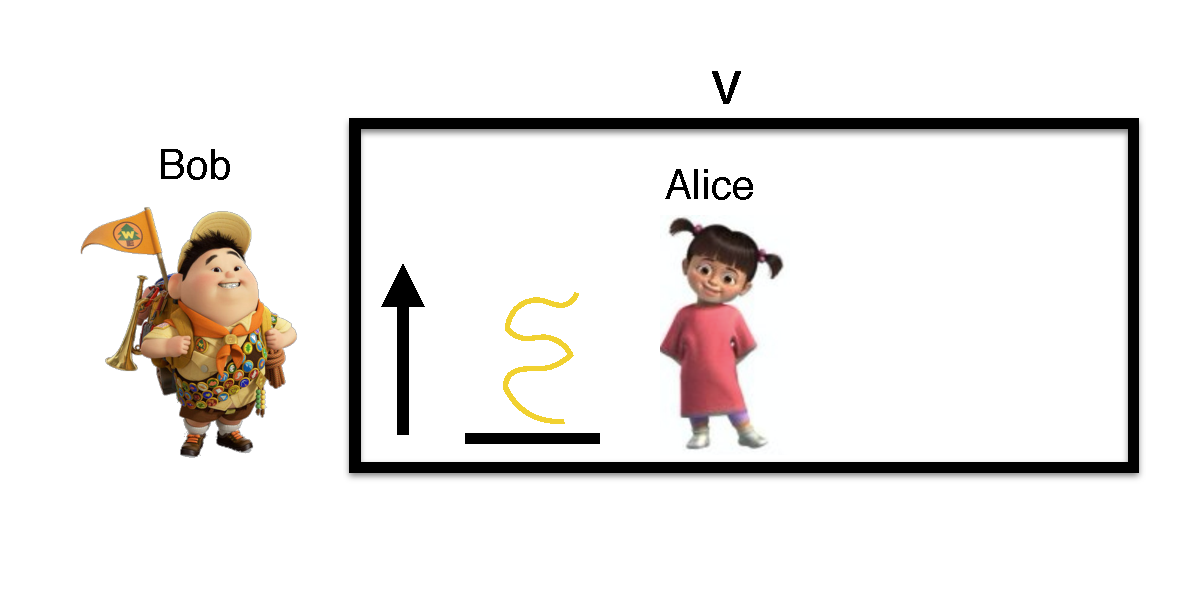
\includegraphics[width=0.25\textwidth, trim={0 0 200pt 0}, clip]{E1.pdf}}
\textbox{E\wref{sec:time-dilation}.1 Light travel and time dilation}{
	Consider Alice and Bob have relative motion against each other, with velocity $v$. Alice carries a candle, which emits light (speed of light is $c$) perpendicular to the motion direction (wrt Alice). 
	\tenum{
		\item What's the speed of this light ray wrt Bob? 
		\item What's the travel direction of this light ray wrt Bob? 
		\item Wrt Bob, the time of Alice slows down. Why doesn't the speed of this light ray slow down? Explain the relation between slower time and speed of light.
	}
}

% Sec 5

\marginnote{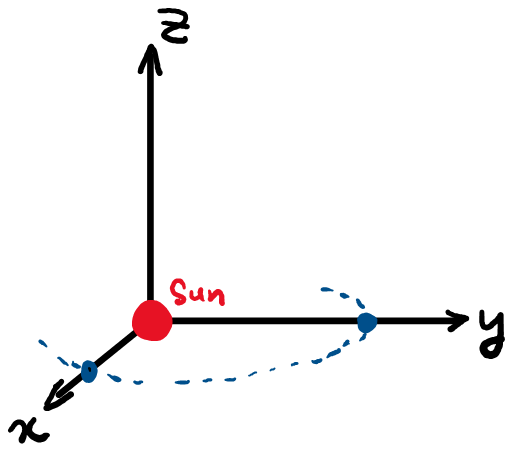
\includegraphics[width=0.25\textwidth, trim={0 2pt 2pt 0}, clip]{earth-sun}} 
\textbox{E\wref{sec:same-time}.1 Spacetime diagram of the sun-earth system}{
	Use the frame that the sun is static, draw a spacetime diagram of the sun's and the earth's motion in $x$-direction (a direction in the earth's orbit plane). Show on this diagram how the sunlight (emitted in the $x$-direction) reaches the earth. The vertical axis is $ct$.
}

\textbox{E\wref{sec:same-time}.2 Spacetime diagram with constant proper acceleration}{
	Alice is moving with constant ``proper acceleration'' in the $x$-direction: $x^2 - t^2=$constant (to simplify the discussion, let's work in one spatial dimension only). Not all light towards the observer can reach Alice. The region where light cannot reach Alice is called the ``Rindler horizon''. Draw a spacetime diagram of Alice's motion and find where the Rindler horizon is.
}

\textbox{E\wref{sec:same-time}.3 What the twin actually sees}{
	Draw the spacetime diagram of the twin paradox and show what the static twin actually sees (i.e. in the order that light reaches his eyes) about the aging of the moving twin (when she was moving outwards and when she was moving back).
}

\textbox{E\wref{sec:same-time}.4 Distance between spaceships.}{
	An observer A is considered at rest in the whole setup of this question. Two spaceships B and C are equidistant to A and are initially also at rest, and the distance between them is $L$. Now A sends a light signal. After receiving the light signal, B and C immediately start to move at a velocity $v$ in the same direction (neglect the period of acceleration). What is the distance between B and C after they are moving? Give your answer wrt A and wrt B, respectively. Hint: draw a spacetime diagram to find out what happened.
}

% Sec 6

\textbox{E\wref{sec:lorentz}.1 Use Lorentz transformation in calculations}{
	Use Lorentz transformation to calculate:
	\tenum{
		\item Time dilation.
		\item Rule contraction.
		\item For two events which happened at the same time wrt Alice, calculate the time difference wrt Bob, given Bob's speed $v$, and the distance between the two events being $L$ wrt Alice. % Lv/c^2
	}
}

\textbox{E\wref{sec:lorentz}.2 Examples of velocity addition}{
	Alice is moving away from Bob with velocity $\vec v =(v,0,0)$, and sending out light rays.
	\tenum{
		\item If the light ray is along $x_A$ direction ($x$ direction wrt Alice), calculate the velocity of the light ray $\vec v_B = (v_{Bx},v_{By},v_{Bz}) $ wrt Bob.
		\item If the light ray is along $y_A$ direction ($y$ direction wrt Alice), calculate the velocity of the light ray $\vec v_B = (v_{Bx},v_{By},v_{Bz}) $ wrt Bob.
	}
}

\textbox{E\wref{sec:lorentz}.3 Speed of light in the media}{
	Consider the speed of light in static air (refractive index $n=1.0003$). How does the speed of light in the air change wrt moving observers moving with speed $v$? How does the speed of light in the air change when there is a wind with speed $v$?
}

% Sec 7

\textbox{E\wref{sec:geometry}.1 The spacetime interval is Lorentz invariant}{
	Show that under Lorentz transformation, the spacetime interval $ds^2$ is unchanged (although $t$ and $x$ change). For simplicity, work in two dimensions $t$ and $x$ only (i.e. no motion or rotation in $y$ and $z$ directions).
}

\textbox{E\wref{sec:geometry}.2 Our motion in spacetime}{
	Show that using proper time, everyone is moving in spacetime (not space) with the same 4-speed (i.e. the size of the 4-velocity $dx^\mu / d\tau$).
}

\textbox{E\wref{sec:momentum-energy}.1 Integrate momentum to get energy}{
	Let us use the relativistic momentum $p=\gamma mv$ to derive the expression of the kinetic energy, in a different way from what we did in class. 

	Consider a ball at rest at $x=0$ with mass m, and act a constant force $F$ on this ball toward the $x$ direction. The ball then accelerates because of the force.

	Note that $F=dp/dt$, and the kinetic energy can be calculated from the work done by the force: 
	\begin{align}
	K= \int_0^{x_1}F~dx= \int_0^{x_1} \left(\frac{dp}{dt}\right)dx=\int_0^{p_1}v~dp=\int_0^{v_1}v~d(\gamma mv)~,
	\end{align}
	where $x_1$, $p_1$ and $v_1$ are the distance, momentum and velocity at a later time $t_1$.

	Continue the calculation and derive the kinetic energy of the ball at time $t_1$.	
}

\textbox{Read Einstein's original papers on relativity}{
	Nowadays Einstein's original papers can be easily found online. For example, \href{https://www.fourmilab.ch/etexts/einstein/specrel/www/}{his first paper}. You will find most parts the paper accessible except that in electrodynamics he used different notations from modern convention. 
}

\printindex

\end{document}
